% Copyright (C) 2004-2007 Jed Brown and Ed Bueler and Nathan Shemonski
%
% This file is part of PISM.
%
% PISM is free software; you can redistribute it and/or modify it under the
% terms of the GNU General Public License as published by the Free Software
% Foundation; either version 2 of the License, or (at your option) any later
% version.
%
% PISM is distributed in the hope that it will be useful, but WITHOUT ANY
% WARRANTY; without even the implied warranty of MERCHANTABILITY or FITNESS
% FOR A PARTICULAR PURPOSE.  See the GNU General Public License for more
% details.
%
% You should have received a copy of the GNU General Public License
% along with PISM; if not, write to the Free Software
% Foundation, Inc., 51 Franklin St, Fifth Floor, Boston, MA  02110-1301  USA

\documentclass[11pt,final]{amsart}

\newcommand{\PISMREV}{205}
\newcommand{\PETSCREV}{2.3.3-p2}

\addtolength\topmargin{-.1in}
\addtolength\textheight{0.3in}
\addtolength{\oddsidemargin}{-.65in}
\addtolength{\evensidemargin}{-.65in}
\addtolength{\textwidth}{1.3in}
\newcommand{\normalspacing}{\renewcommand{\baselinestretch}{1.1}\tiny\normalsize}
\newcommand{\tablespacing}{\renewcommand{\baselinestretch}{1.0}\tiny\normalsize}
\normalspacing

\usepackage{bm,url,xspace,verbatim}
\usepackage{amssymb,amsmath}
\usepackage[final,pdftex]{graphicx}
\usepackage[pdftex]{hyperref}

\newcommand{\ddt}[1]{\ensuremath{\frac{\partial #1}{\partial t}}}
\newcommand{\ddx}[1]{\ensuremath{\frac{\partial #1}{\partial x}}}
\newcommand{\ddy}[1]{\ensuremath{\frac{\partial #1}{\partial y}}}
\renewcommand{\t}[1]{\texttt{#1}}
\newcommand{\Matlab}{\textsc{Matlab}\xspace}
\newcommand{\bU}{\mathbf{U}}
\newcommand{\eps}{\epsilon}
\newcommand{\grad}{\nabla}

\newcommand{\optoptdef}[3]{\vspace{1mm}\noindent \large\texttt{-#1},\,\,\texttt{--#2=}\normalsize\,\,[\textsl{#3}]:\quad}

\newcommand{\rawopt}[1]{\vspace{1mm}\noindent \large\texttt{-#1}\normalsize}
\newcommand{\opt}[1]{\rawopt{#1}\,:\quad}
\newcommand{\optdef}[2]{\rawopt{#1}\,[\textsl{#2}]:\quad}
\newcommand{\optrestrict}[2]{\rawopt{#1}\,[\texttt{#2} \textsl{only}]:\quad}
\newcommand{\optdefrestrict}[3]{\rawopt{#1}\,[\textsl{#2}]\,[\texttt{#3} \textsl{only}]:\quad}
\newcommand{\und}{$\underline{\,\,\,}$}

% note \beginV and \Vend are a pair, but they must be used as follows:
%   \beginV
%      ... stuff
%   \end{verbatim}
%   \Vend
% that is, "\end{verbatim}" still has to appear on a line by itself with no leading spaces
%\newcommand{\Vend}{ \rule{4.6in}{0.1mm}\end{quote} }
%\newcommand{\beginV}{ \begin{quote}\rule{4.6in}{0.1mm}\begin{verbatim} }
\newcommand{\Vend}{ \rule{4.6in}{0.1mm}\end{quote}\normalsize }
%\newcommand{\beginV}{ \small\begin{quote}\rule{4.6in}{0.1mm}\begin{verbatim} }
\newcommand{\beginV}{ \scriptsize\begin{quote}\rule{4.6in}{0.1mm}\begin{verbatim} }

\newcommand{\Vfile}[1]{ \begin{quote}\rule{4.6in}{0.1mm} \verbatiminput{#1} \rule{4.6in}{0.1mm}\end{quote} }

%\makeindex

\title[PISM User's Manual]{\protect{\Large PISM, a \underline{P}arallel \underline{I}ce \underline{S}heet \underline{M}odel:\normalsize} \\ \protect{\Large \bigskip \bigskip User's Manual\normalsize}}

\author[]{Ed $\text{Bueler}^\ast$, Jed Brown, and Nathan Shemonski}

\date{\today.  $\phantom{|}^\ast$\texttt{ffelb\@@uaf.edu}.  Based on PISM revision \PISMREV\,and PETSC release \PETSCREV.  \\\tiny Get PISM by Subversion: \texttt{svn co http://svn.gna.org/svn/pism/trunk pism}.} 

\begin{document}
\maketitle
\thispagestyle{empty}
%\tablespacing

\vspace{2.0in}
\begin{center}
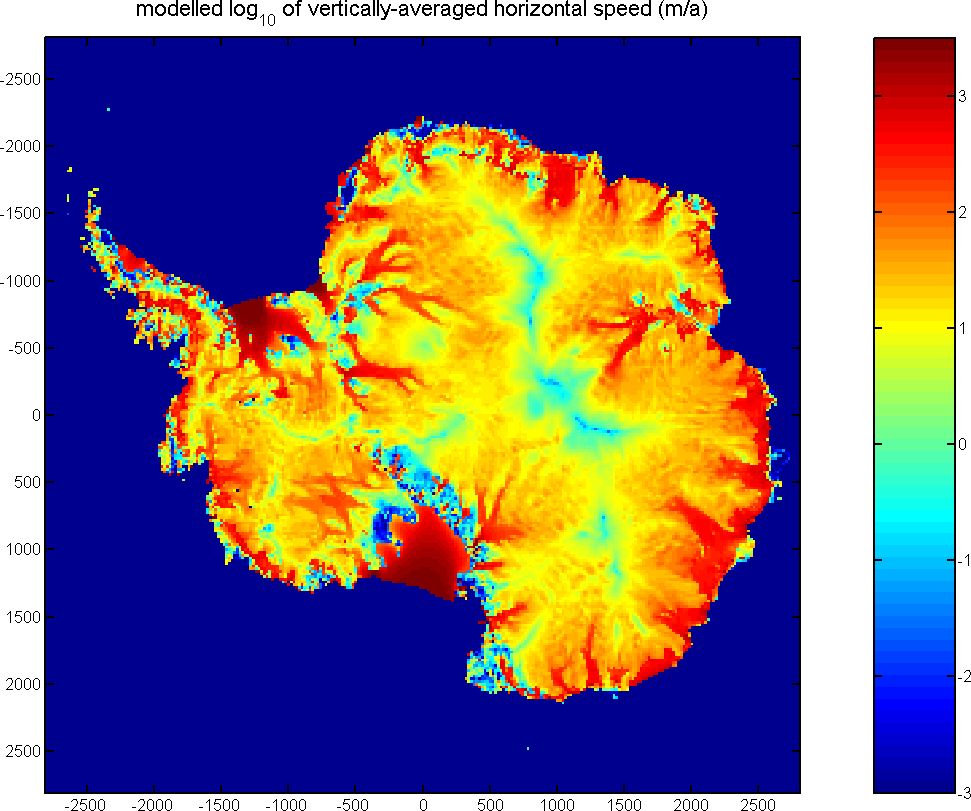
\includegraphics[height=2.7in,keepaspectratio=true]{figs/ant153k_mv100_speed}
\end{center}

\newpage
\phantom{bob}
\vspace{2in}
\begin{quote}
\textsl{Copyright (C) 2004--2007 Ed Bueler and Jed Brown and Nathan Shemonski}
\medskip

\noindent \textsl{This file is part of PISM.}
\medskip

\noindent \textsl{PISM is free software; you can redistribute it and/or modify it under the terms of the GNU General Public License as published by the Free Software Foundation; either version 2 of the License, or (at your option) any later version.}
\medskip

\noindent \textsl{PISM is distributed in the hope that it will be useful, but WITHOUT ANY WARRANTY; without even the implied warranty of MERCHANTABILITY or FITNESS FOR A PARTICULAR PURPOSE.  See the GNU General Public License for more details.}
\medskip

\noindent \textsl{You should have received a copy of the GNU General Public License along with PISM; see \emph{\texttt{pism/COPYING}}; if not, write to the Free Software Foundation, Inc., 51 Franklin St, Fifth Floor, Boston, MA  02110-1301 USA}
\end{quote}
\vspace{1in}
\normalspacing

\centerline{\textsc{Acknowledgements}}
\bigskip

The NASA Cryospheric Sciences Program supported this research with grant NAG5-11371.  Dave Covey and Don Bahls have been the best possible system administrators for the machines on which we have developed PISM.  Thanks to Martin Truffer, Kent Overstreet, and Art Mahoney for helpful comments on the manual and the installation process.  We also want to thank several PISM users whose questions and comments have contributed to improving PISM and this manual.

\newpage
\setcounter{tocdepth}{2}
\tableofcontents


\newpage
\section{Introduction}\label{sect:intro}

Welcome to PISM!

This \emph{User's Manual} describes how to download the PISM source code and install PISM.  It describes how to run it for certain simplified geometry situations.  It illustrates how PISM's numerical codes are verified.  It describes how to use PISM as a modest Greenland ice sheet model or a modest Ross ice shelf model.

But that is all.  Users who want to advance the science of ice sheets will need to go beyond what is described here.  For such users there are two additional documents to know about:
\begin{enumerate}
 \item  The \emph{PISM Reference Manual} (\href{http://www.pism-docs.org/refman.pdf}{\t{www.pism-docs.org/refman.pdf}})
describes the most important pieces of the source code.  It contains, or at least it is intended to contain, the minimum documentation of the PISM source code parts in order to include all the continuum models and numerical methods of PISM.
 \item  The \emph{PISM (HTML) Source Code Browser} (\href{http://www.pism-docs.org/doxy/html/index.html}{\t{www.pism-docs.org/doxy/html/index.html}}) gives a complete view of the class/object structure of the source code.
\end{enumerate}
The \emph{Reference Manual} and the \emph{Source Code Browser} were automatically generated by \verb|doxygen| (\href{http://www.doxygen.org/}{\t{www.doxygen.org}}) from comments in the PISM source code.  Thus they are not as user-friendly as this \emph{User's Manual}.

\vspace{1.5in}
\large
\begin{center}
 \emph{WARNING}:  PISM is an ongoing project.  Ice sheet modeling is complicated and not mature (in 2007, anyway).  Please don't trust the results of PISM or any other ice sheet model without a fair amount of exploration.  Also, please don't expect all your questions to be answered here.  But do write to us with questions: 

\verb|ffelb@uaf.edu|.
\end{center}
\normalsize

\newpage
\section{Installation}\label{sect:install}

\subsubsection*{Installing prerequisities}
\renewcommand{\labelenumi}{\textbf{\arabic{enumi}.}~}
\begin{enumerate}
\item You will need a UNIX system with internet access.  A GNU/Linux environment will be easiest but other UNIX versions have been used successfully.  Package management systems are useful for installing many of the tools below, \emph{but} neither PISM itself nor up-to-date PETSc distributions are currently available in the Debian repositories.  You will need \href{http://www.python.org/}{Python} and \href{http://subversion.tigris.org/}{Subversion} installed, but these are included in all current Linux distributions.  To use the (recommended) graphical output of PISM you will need an  (\href{http://www.x.org/}{X Windows server}.
\item As PISM is currently under rapid development, we distribute it only as compilable source code.  On the other hand, there are several software libraries needed by PISM.  Therefore the ``header files'' for these libraries are required for building PISM.  In particular this means that the ``developer's versions'' of the libraries are needed if the libraries are downloaded from package repositories like Debian.  (In summary, \verb|xorg-dev|, \verb|netcdfg-dev|, \verb|libgsl0-dev|, and \verb|fftw3-dev| are the Debian packages we---the PISM developers---have used in compiling and linking PISM.)

\item PISM uses \href{http://www.unidata.ucar.edu/software/netcdf/}{NetCDF (= \emph{network Common Data Form})} for an input and output file format.   If it is not already present, install it using the instructions at the webpage or using a package management system.

\item PISM uses the \href{http://www.gnu.org/software/gsl/}{GSL (= \emph{GNU Scientific Library})} for certain numerical calculations and special functions.  If it is not already present, install it using the instructions at the webpage or using a package management system.

\item PISM optionally uses the \href{http://www.fftw.org/}{``FFTW'' library (FFTW = \emph{Fastest Fourier Transform in the West})} in approximating the deformation of the solid earth under ice loads \cite{BLKfastearth}.  If you want the functionality of this earth model, which is coupled to the ice flow and which we recommend, install FFTW or check that it is installed already.  If FFTW is \emph{not installed}, however, turn off PISM's attempt to build with it by setting the environment variable \verb|WITH_FFTW=0|.   If this library is absent, all of PISM will work \emph{except} for the bed deformation model described in the paper \cite{BLKfastearth}.

\item You will need a version of \href{http://www-unix.mcs.anl.gov/mpi/}{MPI (= \emph{Message Passing Interface})}.  Your system may have an existing MPI installation, in which case the path to the MPI directory will be used when installing PETSc below.  Otherwise we recommend that you allow PETSc to download \href{http://www-unix.mcs.anl.gov/mpi/mpich2/}{MPICH2} as part of the PETSc configure process (next).  In either case, once MPI is installed, you will want to add the MPI \verb|bin| directory to your path so that you can invoke MPI using the \verb|mpiexec| or \verb|mpirun| command.  For example, you can add it with the statement

\verb|export PATH=/home/user/mympi/bin:$PATH|  \qquad (for \verb|bash| shell)

\noindent or

\verb|setenv PATH /home/user/mympi/bin:$PATH|  \qquad (for \verb|csh| or \verb|tcsh| shell).

\noindent Such a statement can, of course, appear in your \verb|.bashrc|, \verb|.profile|, or \verb|.cshrc| file so that there is no need to retype it each time you use MPI.

\medskip
\centerline{\emph{From now on this manual will assume use of} bash.}
\medskip

\item PISM uses   \href{http://www-unix.mcs.anl.gov/petsc/petsc-2/index.html}{PETSc (= \emph{Portable Extensible Toolkit for Scientific computation})}.  As mentions of this library will occur frequently in this manual, note ``PETSc'' is pronounced ``pet-see''.  Download the PETSc source by grabbing the current gzipped tarball at  
   \centerline{\href{http://www-unix.mcs.anl.gov/petsc/petsc-as/download/index.html}{\t{www-unix.mcs.anl.gov/petsc/petsc-as/download/index.html}}}
PISM requires a version of PETSc which is \texttt{\PETSCREV} or later.\footnote{A Debian package for PETSc may exist, but it should only be used if it is version \texttt{\PETSCREV} or later.}   The ``lite'' form of PETSc is fine if you are willing to depend on an internet connection for accessing the PETSc documentation. 

You should configure and build PETSc \emph{essentially} as described on the  \href{http://www-unix.mcs.anl.gov/petsc/petsc-2/documentation/installation.html}{PETSc installation page}, but it might be best to read the following comments on the PETSc configure and build process first:

\renewcommand{\labelenumii}{(\roman{enumii})}\begin{enumerate}
\item Untar in your preferred location, but note PETSc should \emph{not} be configured (next) using root privileges.  Note that you will need to define the environment variable \verb|PETSC_DIR| before configuring PETSc (next).  For instance, once you have entered the PETSc directory just untarred, \verb|export PETSC_DIR=|$\phantom{!}^\backprime \mathtt{pwd}^\backprime$.  (Note the use of the backprime (\emph{accent-grave}) character, and not the single apostrophe \verb|'|.)

\item When you run the configure script in the PETSc directory, the following options are recommended; note PISM uses shared libraries by default:

\verb|$  ./config/configure.py --with-shared --with-c-support --with-clanguage=cxx|

Note that there is no PISM use of Fortran, and that it is sometimes convenient to have PETSc grab a local copy of BLAS and LAPACK rather than using the system-wide version.  So one may add ``\verb|--with-fortran=0| \verb|--download-c-blas-lapack=1|'' to the other configure options.

\item If there is an existing MPI installation, for example at \verb|/home/user/mympi/|, one can point PETSc to it by adding the option \verb|--with-mpi-dir=/home/user/mympi/|.  The path used in this option must have MPI executables \verb|mpicxx| and \verb|mpicc|, and either \verb|mpiexec| or \verb|mpirun|, in subdirectory \verb|bin/| and MPI library files in subdirectory \verb|lib/|.

\item On the other hand, it seems common that one needs to tell PETSc to download MPI into a place it understands, even if there is an existing MPI.  If you get messages suggesting that PETSc cannot configure using your existing MPI, you might try \verb|configure.py| with option \verb|--download-mpich=1|.

\item Configuration of PETSc for a batch system requires special procedures described at the PETSc documentation site.  One starts with a configure option \verb|--with-batch=1|.  See the ``Installing on machine requiring cross compiler or a job scheduler'' section of the \href{http://www-unix.mcs.anl.gov/petsc/petsc-2/documentation/installation.html}{PETSc installation page}.

\item  Configuring PETSc takes many minutes even when everything goes smoothly.   A value for the environment variable \verb|PETSC_ARCH| will be reported at the end of the configure process; take note of this value.  (Note that a previously installed PETSc can be reconfigured with a new \verb|PETSC_ARCH| if necessary.)

\item  After \verb|configure.py| finishes, you will need to \verb|make all test| in the PETSc directory and watch the result.  If the X Windows system is functional some example viewers will appear; as noted you will need the X header files for this to work.

\item Finally, you will want to set the \verb|PETSC_DIR| and the \verb|PETSC_ARCH| environment variables in your \verb|.profile| or \verb|.bashrc| file.  Also remember to add the MPI \verb|bin| directory to your \verb|PATH|.  For instance, if you used the option \verb|--download-mpich=1| in the PETSc configure, the MPI \verb|bin| directory will have a path like \verb|$PETSC_DIR/| \verb|externalpackages/mpich2-1.0.4p1/$PETSC_ARCH/bin/|.  Therefore the lines 

\small
\verb|export PETSC_DIR=/home/user/petsc-2.3.3-p2/|

\verb|export PETSC_ARCH=linux-gnu-c-debug|

\verb|export PATH=$PETSC_DIR/externalpackages/mpich2-1.0.4p1/$PETSC_ARCH/bin/:$PATH|
\normalsize

\noindent could appear in one of those files.
\end{enumerate}
\end{enumerate}

\medskip
See Table \ref{tab:PISMdepends} for a summary of the dependencies on external libraries, including those mentioned so far.


\subsubsection*{Installing PISM itself}
At this point you have configured the environment which PISM needs.  You are ready to build PISM itself, which is a much quicker procedure!

\begin{enumerate}\setcounter{enumi}{5}
\item \label{getPISMstep} Get the latest source for PISM using the Subversion version control system:

\verb|svn co http://svn.gna.org/svn/pism/trunk pism|

\noindent A directory called ``\verb|pism/|'' will be created.  Note that in the future when you enter that directory, \verb|svn update| will update to the latest revision of PISM.\footnote{Of course, after \t{svn update} you will \t{make} and \t{make install} to recompile and relink PISM.}

\item Build PISM:\footnote{Please report any problems you meet at this build stage by sending us the output: \t{ffelb\@@uaf.edu}.}

\verb|cd pism|

\verb|make|

\verb|make install|

\noindent  Note that the ``\verb|make install|'' puts executables, including \verb|pismd|, \verb|pismr|, \verb|pismv|, and \verb|pisms|, in the \verb|pism/bin/| subdirectory and cleans up the junk from the build process.  ``\verb|make install|'' does \emph{not} require root permission.

\item PISM executables can be run most easily by adding the directories \verb|pism/bin/| and \verb|pism/test/| to your \verb|PATH|.  The former directory contains the major PISM executables while the latter contains several useful scripts.  For instance, this command can be done in the \verb|bash| shell or in your \verb|.bashrc| file:

\verb|export PATH=/home/user/pism/bin/:/home/user/pism/test/:$PATH|
\end{enumerate}
\smallskip


\subsubsection*{Quick tests of the installation}
You are done with installation at this point.  The next few items are recommended as they allow you to observe that PISM is functioning correctly.
\medskip

\begin{enumerate}\setcounter{enumi}{9}
\item \label{serialpismvrun} Try a serial verification run of PISM:

\verb|pismv -test G -y 100|

\noindent If you see some output and a final \verb|Writing model state| \verb|to file 'verify.nc'| \verb|... done| then PISM completed successfully.  Note that at the end of this run you get measurements of the difference between the numerical result and the exact solution \cite{BBL}.

\item Try the MPI four processor version of the above run:

\verb|mpiexec -n 4 pismv -test G -y 100|

\noindent This should work even if there is only one actual processor on your machine, in which case MPI will run multiple processes on the one processor, naturally.  The reported errors should be very nearly the same as the serial run above, but the results should appear faster (if there really are four processors)!

\item Try a verification run on a finer vertical grid while watching the diagnostic views which use Xwindows:

\verb|pismv -test G -Mz 201 -y 2000 -d HTc|

\noindent When using such diagnostic views and \verb|mpiexec| the additional final option \verb|-display :0| is sometimes required to enable MPI to use Xwindows:

\verb|mpiexec -n 2 pismv -test G -Mz 201 -y 2000 -d HTc -display :0|

\item Run a verification test of the ice stream code:

\verb|pismv -test I -Mx 5 -My 401 -verbose|

\noindent This runs a rather different part of the PISM code and then compares the numerical result to the exact solution appearing in \cite{SchoofStream}.

\item Run a Python script for a basic suite of verifications:

\verb|verifynow.py|

\noindent or, on an $N$ processor machine,

\verb|verifynow.py -n |$N$

\noindent If you would like us to confirm that PISM is working as expected please save the one page or so of output from this script and send it to us (\verb|ffelb@uaf.edu|).  See section \ref{sect:verif} for more on PISM verification.
\end{enumerate}
\smallskip

At this stage you can do the EISMINT II simplified geometry experiments and run some verification tests without further downloads.  Subsection \ref{sect:green} is an example of using PISM to model the Greenland ice sheet using freely-downloadable data.  Similarly one can model the Ross ice shelf using free data as described in subsection \ref{sect:ross}.

Naturally, setting up PISM to model real ice sheets will generally require techniques not be covered in this manual.  First of all one usual needs to convert ice sheet data to NetCDF format so that it can be read by PISM.  Actual modeling may also require the writing of additional source code.  As PISM is written in C++, this means writing a derived class of the base class.  (The base class \verb|IceModel| is defined in the source file \verb|pism/src/iceModel.hh|.)  Use of PISM for real ice sheet modeling is something we welcome questions about, and will attempt to help with, but we will not pretend it is routine.

See the PISM Documentation web-page \href{http://www.pism-docs.org/}{\t{www.pism-docs.org}} for links to additional documentation.

A final reminder with respect to installation:  Let's assume you have checked out a copy of PISM using Subversion, as in step \ref{getPISMstep} above.   You can update your copy of PISM to the latest version by \verb|svn update| in the \verb|pism/| directory.  After doing so you will want to \verb|make| and \verb|make install| in order to rebuild the PISM executables using the updated source code files.

Have fun!

\begin{table}[ht]
\caption{Dependencies for PISM, listed alphabetically.  These are needed to build a fully-functional PISM from source and to do all the examples in the manual.}\label{tab:PISMdepends}
\small
\begin{tabular}{@{}llll}\hline
\textbf{Library} & \textbf{Site} & \textbf{Required?} & \textbf{Comment} \\
\textbf{/Program} &  &  &  \\ \hline
FFTW & \href{http://www.fftw.org/}{\t{www.fftw.org}} & \emph{recommended} & if not present set \\
 & & & \quad \verb|WITH_FFTW=0| for PISM build \\
GSL & \href{http://www.gnu.org/software/gsl/}{\t{www.gnu.org/software/gsl}} & \emph{required} &  \\
Matlab & \href{http://www.mathworks.com/}{\t{www.mathworks.com}} & \emph{recommended} & only used for alternate\\
& & & display of results \\
MPI & \href{http://www-unix.mcs.anl.gov/mpi/}{\t{www-unix.mcs.anl.gov/mpi}} & \emph{required} & \\
NetCDF & \href{http://www.unidata.ucar.edu/software/netcdf/}{\t{www.unidata.ucar.edu/software/netcdf}} & \emph{required} & \\
\texttt{numpy} & \href{http://numpy.scipy.org/}{\t{numpy.scipy.org}} & \emph{recommended}  & used in Python scripts in sections \ref{sect:green} and \ref{sect:ross}  \\
PETSc &  \href{http://www-unix.mcs.anl.gov/petsc/petsc-as/}{\t{www-unix.mcs.anl.gov/petsc}} & \emph{required} & version $\ge$ 2.3.3-p2 \\
Python & \href{http://python.org/}{\t{python.org}} & \emph{required} & \\
\texttt{pycdf} & \href{http://pysclint.sourceforge.net/pycdf/}{\t{pysclint.sourceforge.net/pycdf}} & \emph{recommended}  & used in Python scripts in sections \ref{sect:green} and \ref{sect:ross}  \\
Subversion & \href{http://subversion.tigris.org/}{\t{subversion.tigris.org}} & \emph{required} & \\
\hline
\normalsize
\end{tabular}
\end{table}


\begin{table}[ht]
\caption{Additional dependencies for PISM, \protect{\emph{needed only for serious developers of PISM}}, listed alphabetically.  }\label{tab:PISMdepends_superdev}
\small
\begin{tabular}{@{}llll}\hline
\textbf{Library} & \textbf{Site} & \textbf{Comment} \\
\textbf{/Program} &  &  &  \\ \hline
\LaTeX & \href{http://www.latex-project.org/}{\t{www.latex-project.org}} & only used for rebuilding manuals (both this User's Manual  \\
 &  & and the Reference Manual) from source \\
\texttt{doxygen} & \href{http://www.stack.nl/~dimitri/doxygen/}{\t{www.doxygen.org}} & only used for rebuilding the Reference Manual and the \\
 & & Source Code Browser from the source code files \\
\texttt{ruby} & \href{http://www.ruby-lang.org/en/}{\texttt{www.ruby-lang.org}} & only used when changing the NetCDF format \\
 &  & for PISM output files \\
\hline
\normalsize
\end{tabular}
\end{table}


\clearpage\newpage
\section{Getting started}\label{sect:start}

\subsection{Running the EISMINT II tests}  PISM's purpose is the simulation of actual ice sheets.  But actual ice sheet simulations require actual data.\footnote{Actual ice sheet and ice shelf data \emph{are} available on the web as part of the EISMINT intercomparison efforts.  Section \ref{sect:green} is a tutorial on the use of PISM as a Greenland ice sheet or Ross ice shelf flow model using the EISMINT data sets.}  For now, in order to avoid issues of data formats (and data flaws) in a first use of PISM, this section describes how to use PISM for experiment F in the EISMINT II simplified-geometry, thermomechanically-coupled ice sheet model intercomparison \cite{EISMINT00}.  In this experiment one models an angularly-symmetric shallow, grounded ice sheet on a flat bed with relatively cold surface temperatures.  Unfortunately one happens to be approximating an unstable equilibrium of the relevant (thermomechanically-coupled) partial differential equations, so one inevitably gets ``spokes'' in the basal temperature field \cite{BBL,PayneBaldwin,SaitoEISMINT}.

In EISMINT II the prescribed grid has 60 subintervals in each direction, with each subinterval of length 25km.  Thus the total width of the computational box is 1500 km in both $x$ and $y$ directions.  However, PISM always allows choice of the grid in all three dimensions.  A runtime option chooses the number of grid points in each direction; note that the number of points is one greater than the number of subintervals (grid spaces).  The vertical grid is not prescribed in EISMINT II.

We choose the standard 25km grid in the horizontal and use 201 grid points in the vertical for a 25 m (equally-spaced) grid.  Note that the computational box is 5000 m high by default for EISMINT II experiment F in PISM.  Experiment F starts with zero ice, but the center thickness of the ice sheet grows to a peak near 5000 m before decaying to an equilibrium center thickness of about 4400 m.

In EISMINT II all runs are for 200,000 model years.  Here we start with a short 2000 year run for a quicker illustration.  The executable is ``\t{pisms}'', a name which has trailing ``\t{s}'' for the ``simplifed geometry mode'' of PISM:

\small\begin{quote}\begin{verbatim}
$  pisms -eisII F -Mx 61 -My 61 -Mz 201 -y 2000
PISMS (simplified geometry mode)
initializing EISMINT II experiment F ... 
  [computational box for ice: ( 1500.00 km) x ( 1500.00 km) x ( 5000.00 m)]
  [grid cell dimensions     : (   25.00 km) x (   25.00 km) x (   25.00 m)]
running EISMINT II experiment F ...
            YEAR (+     STEP[N$]):     VOL    AREA    MELTF     THICK0     TEMP0
$$$$$      0.000 (+  0.00000[0 ]):   0.000   0.000    0.000      0.000   223.150
$$vtf     60.000 (+ 60.00000[0m]):   0.017   0.628    0.000     30.000   223.150
$$vtf    120.000 (+ 60.00000[0m]):   0.034   0.628    0.000     60.000   223.538
$$vtf    180.000 (+ 60.00000[0m]):   0.051   0.628    0.000     90.000   223.869
...
$$vtf   1980.000 (+ 60.00000[0m]):   0.562   0.631    0.000    990.000   228.487
$$vtf   2000.000 (+ 20.00000[0e]):   0.568   0.631    0.000   1000.000   228.520
done with run ...
Writing model state to file `simp_exper.nc' ... done.
\end{verbatim}
\end{quote}\normalsize
\noindent This should have taken less than 30 seconds.

In a moment we will address the standard output information provided by PISM, as shown above, but for now we simply illustrate how to restart and complete the 200,000 year run.  We see that the model state was stored in a NetCDF file with the \verb|pisms| default name ``\texttt{simp\underline{ }exper.nc}''.  The next run will use a ``\verb|-o|'' option to name the output file.  Also, the above was a single processor run, but let's suppose we have a four processor machine.  (The following should also work fine on a single processor machine  by dropping the prefix ``\verb|mpiexec -n 4|''.)  Let's also run things in the background so we can continue to experiment:

\small\begin{quote}\begin{verbatim}
$  mpiexec -n 4 pisms -eisII F -if simp_exper.nc -y 198000 \
  -o eisIIF200k >> eisIIF.out &
\end{verbatim}
\end{quote}\normalsize

This run will take at least an hour on a four processor computer.  The file \verb|eisIIF200k.nc| (NetCDF format) will appear at the end.  One can, however, view the redirected standard output by \verb|less eisIIF.out| as the job is running in the background.\footnote{\t{top} is a convenient Linux tool to see processor usage during the run.}

If one wants a view of the model state in the midst of this (or any other PISM) run, one can send all running \verb|pisms| processes a signal which causes PISM to write out the model state: \verb|pkill -USR1 pisms|.  The PISM model state is then saved in a NetCDF file with name \verb|pism-|\emph{year}\verb|.nc| using the year at that time step.  On the other hand, if one terminates the run with \verb|pkill -TERM pisms| then the run will stop and save the model state using the \verb|-o| specified name even though it will not be the state at the end of a completed run.\footnote{Indeed, if the reader is impatient or has a single processor machine and doesn't want to wait more than an hour, the experiment F run can be terminated by \t{pkill -TERM pisms} after about 50,000 model years and the basic model result will be similar to that at 200,000 years.}  (See subsection \ref{subsect:signal} for a more complete description of how PISM catches signals.)

While the four process run continues in the background, let's view the model state during a few time steps by starting from the saved 2000 year state.  We use PISM's ``diagnostic viewers'', which requires X Windows:

\small\begin{quote}\begin{verbatim}
$  pisms -eisII F -if simp_exper.nc -y 200 -d HTt
PISMS (simplified geometry mode)
initializing from NetCDF format file  simp_exper.nc  ...
  [computational box for ice: ( 1500.00 km) x ( 1500.00 km) x ( 5000.00 m)]
  [grid cell dimensions     : (   25.00 km) x (   25.00 km) x (   25.00 m)]
running EISMINT II experiment F ...
            YEAR (+     STEP[N$]):     VOL    AREA    MELTF     THICK0     TEMP0
$$$$$   2000.000 (+  0.00000[0 ]):   0.568   0.631    0.000   1000.000   228.520
$$vtf   2060.000 (+ 60.00000[0m]):   0.585   0.631    0.000   1030.000   228.616
$$vtf   2120.000 (+ 60.00000[0m]):   0.602   0.631    0.000   1060.000   228.710
$$vtf   2180.000 (+ 60.00000[0m]):   0.619   0.631    0.000   1090.000   228.804
$$vtf   2200.000 (+ 20.00000[0e]):   0.625   0.631    0.000   1100.000   228.834
done with run ... 
Writing model state to file `simp_exper.nc' ... done.
\end{verbatim}
\end{quote}\normalsize

Three figures should appear and be refreshed at each time step.  One figure is a map-plane view of thickness, another is a map-plane view of the basal temperature in Kelvin, and third there is a graph of height above the bed versus temperature.  

When the full 200,000 year run finishes, one can continue the run and watch its evolving state by

\verb|pisms -eisII F -if eisIIF200k.nc -d HTt|

\noindent A result like that shown in figure \ref{fig:screenshot} will appear.

\begin{figure}[ht]
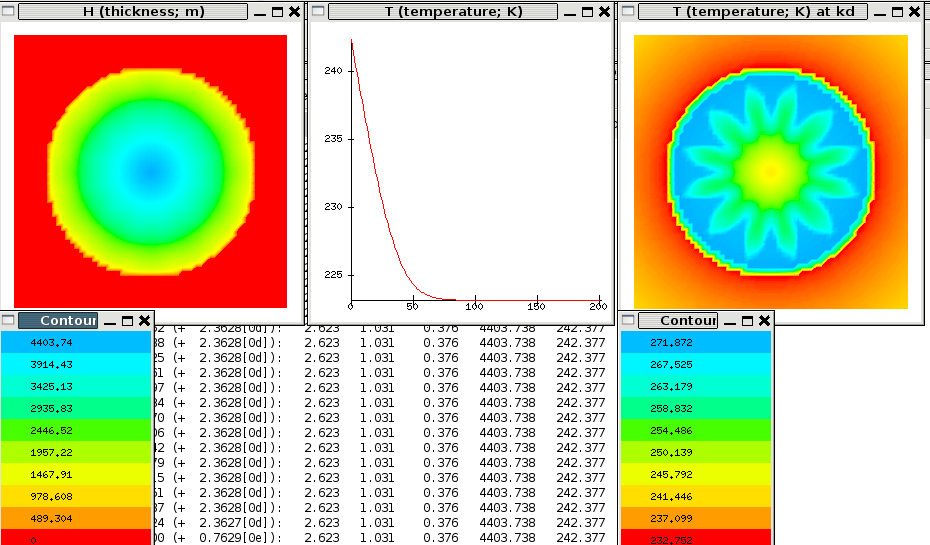
\includegraphics[height=3.2in,keepaspectratio=true]{figs/eisIIFshot}
\caption{Diagnostic figures at the end of a 200,000 year EISMINT II experiment F run, showing the famous spokes.}
\label{fig:screenshot}
\end{figure}

At each time step PISM shows a summary of the model state using a few numbers.  The format of the summary is

\small\verb|           YEAR (+    STEP[N$]):     VOL    AREA    MELTF     THICK0     TEMP0|\normalsize

\noindent The first five columns are flags telling the user which quantities are being updated at that time step.  A dollar sign appears if the quantity does not update.  From the left the positions are: [\t{b\$}] for bed elevation, [\t{vV\$}] for velocity, [\t{g\$}] for grain size, [\t{t\$}] for temperature and age (which are always updated together), and [\t{f\$}] for surface elevation.   (That is, an ``\verb|f|'' in the last column means a step of the flow or mass conservation equation has occurred.  Regarding the two possible velocity flags, a lower case ``\texttt{v}'' indicates that the 3D velocity field has been updated, e.g.~as needed for the advection of temperature, while uppercase ``\texttt{V}'' indicates that only the vertically-averaged velocity, and the associated diffusivity, has been updated.)

The time (``\t{YEAR}'') and time step (``\t{STEP}'') are in years.\footnote{At the beginning of the EISMINT II experiment F run the ice has small thickness so the time step is 60 years because that is the default maximum time step.  Later in the experiment F run, after 5000 years, for instance, the time step is made smaller by the adaptive time-stepping mechanism in PISM.  See subsection \ref{subsect:adapt} for more on adaptive time-stepping.}  A small whole number and a single character flag appear in square brackets after the time step, and these explain what part of the adaptive time-stepping scheme was used to determine the time step.  For instance, ``\t{m}'' means that the step was the maximum allowed, ``\t{e}'' means that the time step was shortened to hit the end of the specified run, ``\t{d}'' means the step was determined by the diffusivity of the flow equation \cite{BBL}, and ``\t{c}'' means the CFL condition limited the time step \cite{BBL,MortonMayers}.  The small integer before this single character flag is related to the \verb|-tempskip| mechanism; see sections \ref{sect:options} and \ref{sect:simp} for further description and examples of this mechanism.

The next three columns in the summary report the volume of the ice in $10^6 \,\text{km}^3$, the area covered by the ice in $10^6\,\text{km}^2$, and the basal melt fraction, that is, the fraction of the ice area where the basal homologous temperature is above $273.0$ (i.e.~slightly lower than the triple point).  The next two columns ``\texttt{THICK0}'' and ``\texttt{TEMP0}'' are values at the center of the computational domain of the map plane, namely the thickness in meters and the basal absolute temperature in Kelvin.  These five numbers are also the ones reported in the tables in \cite{EISMINT00}, which is sometime useful for comparison.  This summary of the model state can be made more verbose by using the option \verb|-verbose|.

For more on the EISMINT II experiments see section \ref{sect:simp}.

\subsection{Visualizing the results}  There are three basic modes for visualizing the various quantities in PISM, namely using runtime viewers, visualizing final output model state NetCDF files, and visualizing final output \Matlab files for individual variables.

At runtime, various viewers can be specified by options of the form \verb|-d |\emph{letters} or \verb|-dbig |\emph{letters}; the latter option shows larger windows but is otherwise identical.  See Appendix C for the possible single letter names of each runtime viewer.  These viewers are updated at each step and work under Xwindows.  The format is limited by the style of PETSc viewers, but these viewers generally suffice for visualizing an ongoing PISM run.  Note that some diagnostic viewers show slices of three-dimensional quantities in slices parallel to the bed.  They are controlled by the option \verb|-kd|.  Those which show ``soundings'' are controlled by the options \verb|-id|, \verb|-jd|; see Appendices \ref{sect:options} and \ref{sect:viewers}.

When a PISM run is finished the state of the model is output in NetCDF format.  The name can be specified by the option \verb|-o|, so \verb|-o foo| writes the NetCDF file \verb|foo.nc|.  NetCDF files can be viewed or modified with a variety of tools, some of which are mentioned in table \ref{tab:NetCDFview}.  The PISM developers find \t{ncview} to be the fastest routine way to look at PISM output files.

When a PISM run is finished \emph{and the user has specified options of the form} \verb|-mato foo| and \verb|-matv |\emph{letters}, PISM saves the variables named by the letters in a \Matlab-readable file \verb|foo.m|.  The single letter arguments to \verb|-d| and \verb|-matv| are generally the same.  See Appendix \ref{sect:viewers}.

\begin{table}[ht]
\caption{Tools for viewing and modifying NetCDF files.}\label{tab:NetCDFview} 
\small
\begin{tabular}{@{}llll}\hline
\textbf{Tool} & \textbf{Site} & \textbf{Function}\\ \hline
\verb|ncdump| & \emph{included with any NetCDF distribution} & dump as text file \\
\verb|ncview| & \scriptsize\url{http://meteora.ucsd.edu/~pierce/ncview_home_page.html}\small & quick graphical view \\
\verb|ncBrowse| & \href{http://www.epic.noaa.gov/java/ncBrowse/}{\t{www.epic.noaa.gov/java/ncBrowse/}} & quick graphical view \\
\verb|IDV| & \href{http://www.unidata.ucar.edu/software/idv/}{\t{www.unidata.ucar.edu/software/idv/}} & more complete visualization \\
\verb|NCO| = NetCDF & \href{http://nco.sourceforge.net/}{\t{nco.sourceforge.net/}} & sophisticated manipulations \\
\quad Operators & & \quad at command line\\
\hline
\multicolumn{3}{c}{See \href{http://www.unidata.ucar.edu/software/netcdf/docs/software.html}{\t{www.unidata.ucar.edu/software/netcdf/docs/software.html}} for additional tools.} \\
\end{tabular}
\normalsize
\end{table}

\subsection{Evolution runs versus ``diagnostic'' runs}  The main goal of a numerical ice sheet model like PISM is to be a dynamical system which evolves over time as similarly as possible to the modeled ice sheet.  Such a goal assumes one starts with the right initial conditions and that one has the right climate and other inputs at each time step (i.e.~boundary conditions).  Underlying an ice sheet model like PISM are evolution-in-time partial differential equations.  The natural execution mode for a numerical ice sheet model is to take small time steps in approximating these differential equations; ``small time steps'' could mean several years, of course.  We will describe this usual time-stepping behavior as an ``evolution run.''

Much of ice sheet, stream, and shelf modeling, however, requires ``diagnostic'' solution only of the partial differential equations which determine the velocity field.  These are the balance of momentum equations for a slowly flowing fluid \cite{Fowler}.  (As explained in the next section, the ``shallow ice approximation'' which underlies the EISMINT II experiments is only one of two forms of the balance of momentum equations solved by PISM.  The other is the ``shallow shelf approximation''.)  In a diagnostic computation of this type the temperature field and certain basal conditions, such as the yield stress of the till for instance, are held fixed.  In summary, the goal of a ``diagnostic run'' is to compute the velocity field; this will be the definition used from now on in this manual.

On the other hand, the NetCDF model state saved by PISM at the end of an evolution run does not, by default, contain the three-dimensional velocity field.  Instead, it contains those variables which are needed to restart the run, especially the geometry (thickness and bed elevation) and the ice temperature field.  For this and other reasons there is a separate executable \verb|pismd| which only does a diagnostic computation of velocity.  It saves the full three-dimensional velocity field but it does not do time-stepping.

For example, using the quantities already computed in this section, try

\verb|pismd -if eisIIF200k.nc -o eisIIF200k_fullvels|

\noindent The result of this command is a NetCDF file \verb|eisIIF200k_fullvels.nc| which contains the full three-dimensional velocity field in the scalar NetCDF variables \verb|u|, \verb|v|, and \verb|w|.

The velocity field saved by \verb|pismd| is the one which would be computed at the \emph{next} time step in an evolution run.  That is, if we also run

\verb|pisms -eisII F -if eisIIF200k.nc -y 0.1 -o eisIIF200k_plus|

\noindent then the horizontal velocity field computed in this single time step run is the same as that saved in \verb|eisIIF200k_fullvels.nc|.\footnote{For this example, one can use a NetCDF Operator to check that the two saved NetCDF files really correspond to the same vertically-averaged horizontal velocity field; just do \t{ncdiff -v cbar} \dots}  One can also force PISM to save the full velocity field at the end of a time-stepping run using the option \verb|-full3Dout|.  Either way, saving the full velocity field roughly doubles the size of the output model state NetCDF file.

Subsection \ref{sect:ross} describes the use of \verb|pismd| in modeling the Ross ice shelf.  Indeed, ``ice shelf modeling'' has historically meant diagnositic and not evolution computations \cite{MacAyealetal,HumbertGreveHutter}.




\clearpage
\newpage
\section{Ice dynamics in PISM}\label{sect:dynamics}

\subsection{Two models of ice flow: slow versus fast, but always shallow}  PISM can numerically solve two significantly different sets of equations which determine the velocity field within the ice.  In both cases the geometry of the ice, the temperature field within the ice, and the stress condition at the base of the ice are included into balance of momentum equations to determine the flow.  But there are two different versions of the balance of momentum equations:\begin{itemize}
\item the shallow ice approximation (SIA) \cite{Hutter}, which describes ice flow as a function of the driving shear stresses of classical glaciology (i.e.~in planes parallel to the geoid) \cite{Paterson}, and
\item the shallow shelf approximation (SSA) \cite{WeisGreveHutter}, which describes a membrane-type flow driven by longitudinal stress gradients \cite{Morland,MacAyeal,SchoofStream}.
\end{itemize}
PISM numerically solves both the SIA and SSA equations in parallel.  The SIA equations are, as a rule, easier and quicker to numerically solve than the SSA.  Certainly the SIA equations are easier to parallelize.

The SIA equations can confidently be applied to those grounded parts of ice sheets for which the basal ice is frozen to the bedrock and the bed topography is relatively slowly-varying the map-plane \cite{Fowler}.  PISM can solve these equations with additional basal shear stress dependent sliding, but this has decreasing validity as the contribution of the basal sliding to the total flow velocity increases.

The SSA equations can confidently be applied to large floating ice shelves because such shelves have small depth-to-width ratio and because there is no shear stress at the base of the floating ice \cite{Morland,MorlandZainuddin}.

Ice sheets have faster-flowing \emph{grounded} parts, however.  These are usually called ``ice streams'' or ``outlet glaciers''.  Such features appear at the margin of, and even well into the interior of, the Greenland \cite{Joughinetal2001} and Antarctic \cite{BamberVaughanJoughin} ice sheets.  Describing these faster-flowing grounded parts of ice sheets requires something more than the SIA.  Ultimately one might use the full Stokes equations which represent the balance of \emph{all} tensor components \cite{Fowler}.  Alternatively one might use a ``higher-order'' but still shallow stress balance \cite{Blatter}.

Though they apply with greatest confidence to ice shelves, one may apply the SSA equations with additional basal resistance terms to grounded ice.  This was justified in the context of the Siple Coast ice streams of Antarctica by MacAyeal \cite{MacAyeal,HulbeMacAyeal} using a linearly-viscous model for the underlying till.  A free boundary problem with essentially the same (SSA) balance equations is also the Schoof \cite{SchoofStream} model of ice streams.  In Schoof's model ice streams emerge in those parts of the ice sheet where there is plastic till failure; see also \cite{SchoofTill}.

These are the models PISM uses to describe faster-flowing ice, namely the SSA with either linearly-viscous or plastic till.  In the former case the balance of momentum equations are solved as a fixed-boundary problem (at a particular time step), and thus the locations and extent of ice streams must be determined by some other criterion.  In the latter case the locations of ice streams is determined as part of the free boundary problem (for the balance of momentum equations).

As noted, both the SIA and SSA models are \emph{shallow} approximations.  That is, the partial differential equations in these two approximations come by (different) small-parameter arguments, based on a small depth-to-width ratio, from the Stokes equations of a non-Newtonian fluid.  For this small-parameter argument in the SIA case see \cite{Fowler}.  For the corresponding SSA argument, see the appendices of \cite{SchoofStream}.\footnote{The references are, of course, the right place to examine the continuum equations and their physical motivation.  This manual naturally avoids serious discussion of continuum models.}

The actual numerical solution of the SSA is not done by default for the executables \verb|pismr|, \verb|pismd|, or \verb|pisms|.  The user must add the flag \verb|-ssa|.

One must generally decide which parts of the grounded ice sheet are modeled by the SIA and which by the SSA.  This is true for the linearly-viscous till model \cite{MacAyeal} but also in cases where Schoof's plastic-till model is only applied to part of the grounded ice sheet.  The rest of this section largely focuses on how the user makes this choice in practice when using PISM.

One way is to specify a \emph{mask}.  Within PISM, each grid point in the horizontal grid is either SIA \emph{or} SSA.  Each horizontal grid point corresponds to a whole vertical column of grid points in the three-dimensional grid, so it is perhaps better to say that \emph{each vertical column} of ice, centered at a horizontal grid point, is either SIA or SSA.  When ice is floating (according to the usual floatation criterion \cite{WeisGreveHutter}), the horizontal grid point is automatically marked as SSA.

The transition from SIA to SSA flow is an internal boundary within the model domain.  Along this boundary, the numerical schemes in PISM attempt to maintain these continuum facts:
\renewcommand{\labelenumi}{\textbf{\roman{enumi})}~}
\begin{enumerate}
\item continuity of the \emph{vertically-averaged} horizontal velocity field across the SIA--SSA transition,
\item conservation of mass \emph{in the map plane} across the SIA--SSA transition, and
\item conservation of energy in three dimensions across the SIA--SSA transition.
\end{enumerate}
Of course the statement ``attempt to'' maintain is important because PISM does not have exact representations of any continuous functions at all.  It only ``knows'' their gridded numerical approximations.  See section \ref{sect:over} of this manual, and the \emph{PISM Reference Manual}, for additional comments and references on the continuum models and numerical schemes in PISM.

\subsection{The flow-type mask} \label{subsect:mask}  PISM always keeps track of a ``flag'' for flow-type at each point in the map-plane (two-dimensional) grid.  This flow-type flag can potentially change at each time step.  We call the array in which this flow-type flag is stored the ``mask''.  There are four valid values for the mask (at this time), shown in Table \ref{tab:maskvals}.

\begin{table}[ht]
\caption{Values for the PISM mask.}\label{tab:maskvals} 
\small
\begin{tabular}{@{}llll}\hline
\textbf{Value} & \textbf{Name} & \textbf{Meaning}\\ \hline
1 & \verb|MASK_SHEET| & ice is grounded and the SIA is applied \\
2 & \verb|MASK_DRAGGING| & ice is grounded and the SSA is applied if option \verb|-ssa| is given \\
3 & \verb|MASK_FLOATING| & ice is floating and the SSA is applied if option \verb|-ssa| is given \\
7 & \verb|MASK_FLOATING_OCEAN0| & same as \verb|MASK_FLOATING| but the point was ice free ocean at  \\
 & & initialization of the model by \verb|-bif|  \\
\hline\end{tabular}
\normalsize
\end{table}

\begin{figure}[ht]
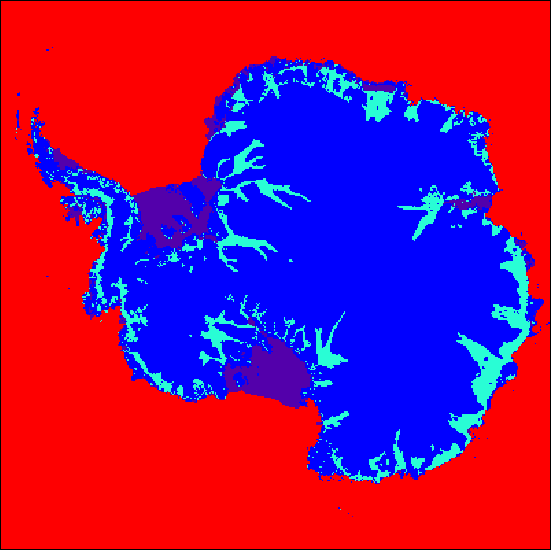
\includegraphics[height=3.2in,keepaspectratio=true]{figs/ant_mask}
\caption{A mask for flow-type for Antarctica.  Red is for ice-free ocean (\t{MASK\_FLOATING\_OCEAN0}), purple is for ice shelves (\t{MASK\_FLOATING}), pale blue is for ice streams (\t{MASK\_DRAGGING}), and darker blue is for interior ice modeled by the SIA (\t{MASK\_SHEET}).}
\label{fig:ant_mask}
\end{figure}

An example mask is shown in Figure \ref{fig:ant_mask}.  The generation of such a mask must include a decision on where the grounded ice can be treated as an ice stream or outlet glacier.  In this case it has been generated using ``balance velocities'' computed from a certain highly simplified flow model \cite{BamberVaughanJoughin} and then a criterion on sliding sufficient to constitute streaming.

Procedures for generating such masks are not, for now, documented.


\subsection{Schoof's plastic till free boundary problem for ice streams} \label{subsect:plastic}    In \cite{SchoofTill} C.~Schoof proposes a model for plastic failure of the basal till under flowing ice, and in \cite{SchoofStream} he recognizes this as a free boundary problem for the SSA.  The result is a model for emergent ice streams within a larger ice sheet and ice shelf system.  It explains the existence of ice streams by a combination of the plastic failure of the till and the SSA approximation of the balance of momentum.

PISM implements Schoof's model as an alternative to the direct ``mask'' scheme described above.  The user gives the options \verb|-ssa -plastic| to turn on this model.  All grounded points are marked as SSA (i.e.~as \verb|MASK_DRAGGING|).  At these points a yield stress is computed from the amount of stored basal water, a thermodynamic quantity, and from a (generally) spatially-varying till strength.  See the description of option \verb|-plastic| in Appendix A for a detailed description of the yield stress computation.

\subsubsection*{A plastic till modification of EISMINT II experiment I}  To demonstrate the implementation we describe an example based on EISMINT II experiment I.  This particular experiment is documented in \cite{EISIIdescribe}.  Experiment I was not, however, discussed in the published intercomparison because the results for experiment I were ``straightforward results with little variability between groups'' \cite{EISMINT00}.  Note that Section \ref{sect:simp} describes using PISM to perform all the EISMINT II experiments documented in \cite{EISIIdescribe}, including experiment I.

Experiment I is identical to experiment A except for having ``trough'' bed topography.  This bed is shown in Figure \ref{fig:eis2I}.  As specified, experiment I has nothing to do with the SSA equations or plastic till failure, and indeed there is no basal motion at all.  However, we use it to build an ice sheet which ``ought'' to have an ice stream, that is, along the trough.

\begin{figure}[ht]
\includegraphics[height=3.1in,keepaspectratio=true]{figs/eis2Ibed} 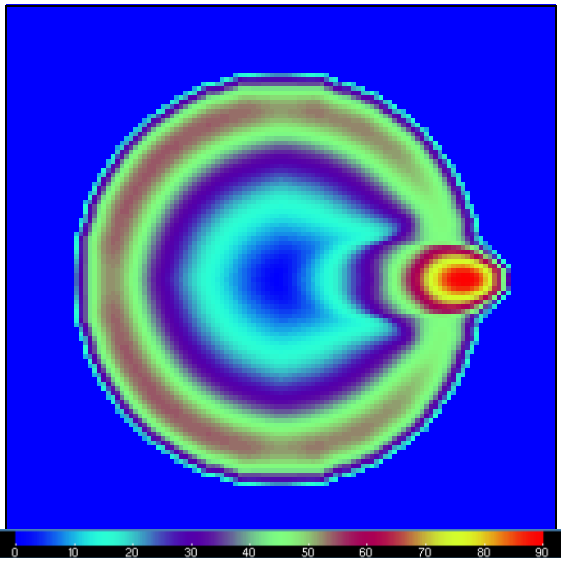
\includegraphics[height=3.1in,keepaspectratio=true]{figs/cbar_eis2I}
\caption{Left: Bed elevation for EISMINT II experiment I.  Most of the bed is a plateau at 1000 m (red), but the trough descends to zero elevation (blue).  Right: The vertically-averaged horizontal speeds at the end of a 200k year run using EISMINT II experiment I as specified, that is, with only the SIA for flow.  The grid is finer than is standard for EISMINT II (12.5 km instead of 25 km).  Speeds vary from 0 (blue) to 90 (red) m/a.}
\label{fig:eis2I}
\end{figure}

The following runs take a while (hours to days).  There is a script \verb|test/eis2Iplastic.sh| which contains the following sequence and allows choice of the number of processors.

First we build the ice sheet for experiment I for 180,000 model years on the standard EISMINT II grid, which is relatively coarse with horizontal spacing of $25$ km.  Note that this run and the next parallelize well, so they will go quickly on (for instance) 10 to 40 processors:

\verb|pisms -eisII I -Mx 61 -My 61 -Mz 201 -y 180000 -o eis2I180k|

\noindent Note that a significant fraction of the base is at the pressure-melting temperature.   At this point the effective thickness of the basal water is zero because stored basal water is not part of the EISMINT II model.  So we now turn on the part of the thermodynamical model which keeps track of stored basal water.  Also we refine the grid to 12.5 km spacing, we run for the remaining 20,000 model years to complete the EISMINT II specified 200k year run, and we save full three-dimensional velocities at the end of the model run:

\verb|pisms -eisII I -Mx 121 -My 121 -Mz 301 -regrid eis2I180k.nc -regrid_vars TBHh \|

\verb|   -y 20000 -track_Hmelt -f3d -o eis2I_fine_wmelt|

\noindent Through use of \verb|ncview| on the output file, for instance, we see that the effective thickness of the till water has increased to its maximum of 2 m in the area where the base is at the pressure-melting temperature.  In particular there is 2 m of stored basal water at the base of the ice in the majority of the trough part of the ice sheet.

Now we turn on Schoof's plastic till ice stream model.  Because we are solving the SSA this part is substantially slower (per model year) and it harder to parallelize; it probably should be run on at most 16 processors:

\verb|pisms -eisII I -if eis2I_fine_wmelt.nc -ssa -plastic -super -verbose \|

\verb|   -till_phi 20.0,5.0 -y 5 -f3d -o eis2I_plastic5|


\subsubsection*{Test I is an exact solution}  PISM's solution of Schoof's plastic till free boundary problem is also solved by test I in the verification suite.  It is based on the exact solution published in \cite{SchoofStream}.  It is a single diagnostic computation of the velocity of a single highly-simplified ice stream.  Here is an example run with some viewers:

\verb|pismv -test I -Mx 5 -My 500 -d ncqu -verbose|

\noindent The boundary conditions are a uniform slab of ice on a bed with constant slope, but with a central low in the particular, defined distribution of till yield stress.  There is zero yield stress at the very center.  Thus the center of the slab slides, and thus the ice flows under the SSA equations, because of the plastic failure, while at the margins the base of the ice does not slide.  That is, we have a single simplified ice stream, and in fact the solution only has interesting variation in the $y$ direction (across slope).  PISM's job is to compute the width and speed of the ice stream, ``knowing'' only the ice thickness, bed slope, and yield stress distribution.  In this case we have the exact solution with which to compare the numerically-computed velocities.  This test, and convergence of PISM's numerical solution of it under grid refinement, are addressed in section \ref{sect:verif}.





%\clearpage
%\newpage
\section{Initialization and inverse problems: ``bootstrapping'' PISM}\label{sect:boot}  [THIS SECTION IS TO BE ADDED; see subsection \ref{sect:green} as an example of bootstrapping;  note \cite{JoughinMacAyealTulaczyk} is a representative inverse modeling result which could be incorporated in a forward model when using the SSA for ice streams if the Schoof plastic till model is \emph{not} used]


\clearpage
\newpage
\section{More on usage}\label{sect:usage}

\subsection{The PISM coordinate system and grid} \label{subsect:coords} PISM does all simulations in a computational box which is rectangular in the PISM coordinates.

The coordinate system has horizontal coordinates $x,y$ and a vertical coordinate $z$.  The $z$ coordinate is measured positive upward from the base of the ice and it is exactly opposite to the vector of gravity.  The surface $z=0$ is the base of the ice, however, and thus is usually not horizontal in the sense of being parallel to the geoid.   The surface $z=0$ is the base of the ice both when the ice is grounded and when the ice is floating.

Bed topography is, of course, allowed.  In fact, when the ice is grounded, the true physical vertical coordinate $z'$, namely the coordinate measure relative to a reference geoid, is given by $z'=z+b(x,y)$ where $b(x,y)$ is the bed topography.  The surface $z'=h(x,y)$ is the surface of the ice.  Thus in the grounded case the equation $h(x,y)=H(x,y)+b(x,y)$ applies if $H(x,y)$ is the thickness of the ice.

In the floating case, the physical vertical coordinate is $z'=z-(\rho_i/\rho_s) H(x,y)$ where $\rho_i$ is the density of ice and $\rho_s$ the density of sea water.  Again $z=0$ is the base of the ice, which is the surface $z' = -(\rho_i/\rho_s) H(x,y)$.  The surface of the ice is $h(x,y) = (1-\rho_i/\rho_s) H(x,y)$.  All we know about the bed elevations is that they are below the base of the ice when the ice is floating.  That is, the \emph{floatation criterion} $-(\rho_i/\rho_s) H(x,y) > b(x,y)$ applies.

The computational box can extend downward into the bedrock.  As $z=0$ is the base of the ice, the bedrock corresponds to negative $z$ values regardless of the sign of its true (i.e.~$z'$) elevation.

The extent of the computational box, along with its bedrock extension downward, is determined by four numbers \t{Lx}, \t{Ly}, \t{Lz}, and \t{Lbz}.  The first two of these are half-widths and have units of kilometers when set by options or displayed.  The last two are vertical distances in the ice and in the bedrock, respectively, and have units of meters.  See the sketch in figure \ref{fig:rectilinearbox}.

\begin{figure}[ht]
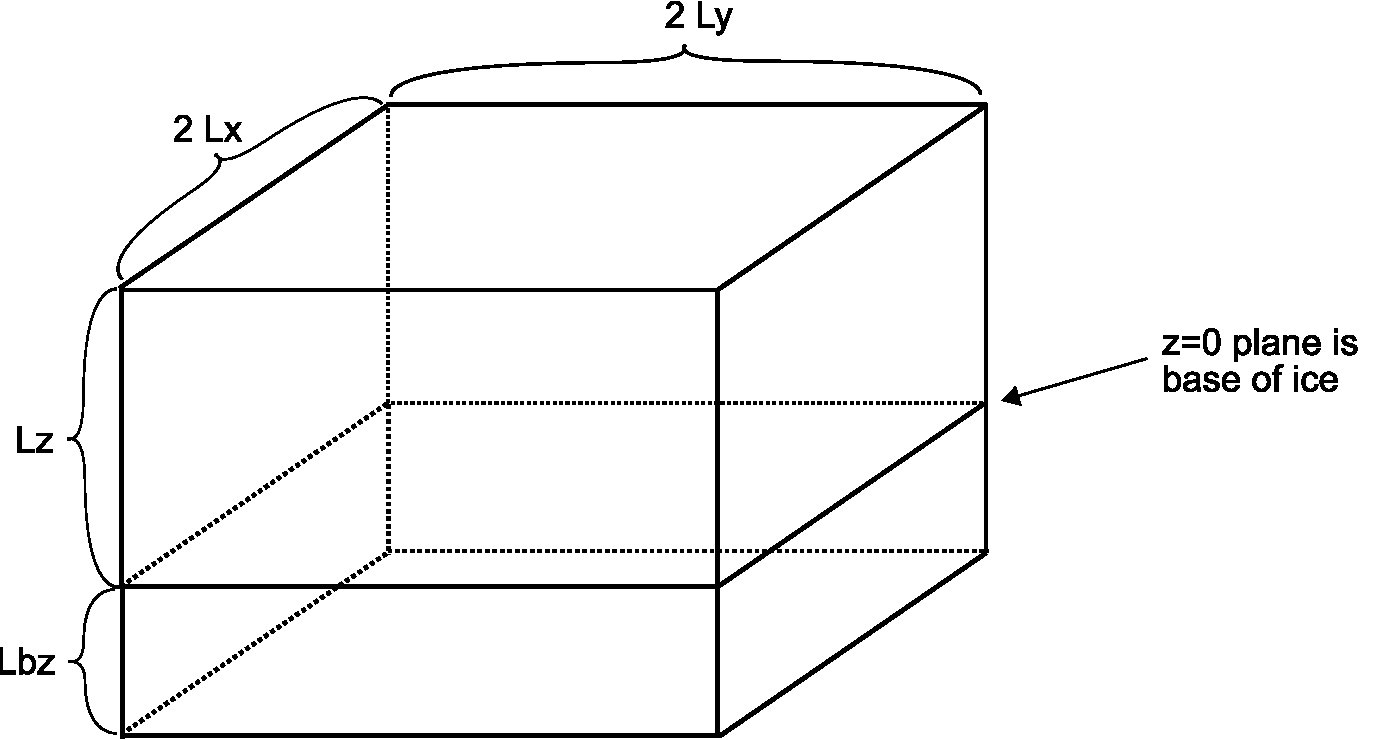
\includegraphics[width=4.0in,keepaspectratio=true]{figs/rectilinearbox}
\caption{PISM's computational box.}
\label{fig:rectilinearbox}
\end{figure}

The extent of the computational box for the ice is directly controlled by the options \t{-Lx}, \t{-Ly}, and \t{-Lz} as described in the Runtime options section.  As noted \t{-Lx} and \t{-Ly} options should include values in kilometers while \t{-Lz} should be in meters.

The PISM grid covering the computational box is equally spaced in each of the three dimensions.  Because of the bedrock extension, the grid of points is described by four numbers, namely the number of grid points in the $x$ direction, the number in the $y$ direction, the number in the $z$ direction within the ice, and the number in the $z$ direction within the bedrock.  These are specified by options \verb|-Mx|, \verb|-My|, \verb|-Mz|, and \verb|-Mbz|, respectively, as described in the Runtime options section.  The defaults for these four values are 61, 61, 31, and 1, respectively.  Note that \verb|Mx|, \verb|My|, \verb|Mz|, and \verb|Mbz| all indicate the number of grid \emph{points}.  Therefore the number of grid \emph{spaces} are, respectively, 60, 60, 30, and 0 (zero) in the default case.  Note that the lowest grid point in a column of ice, that is the one at $z=0$, coincides with the highest grid point in the bedrock.  Also \verb|Mbz| must always be at least one.

The distance \t{Lbz} is controlled by specifying the number \verb|Mbz| of grid points in the bedrock, noting that the vertical spacing \t{dz} is the same within the ice and within the bedrock.  To avoid conflicts, the distance \t{Lbz} cannot be set directly by the user.  In particular, $\text{\t{Lbz}}=\text{\t{dz}}\,(\text{\t{Mbz}}-1)$ while $\text{\t{dz}} = \text{\t{Lz}} / (\text{\t{Mz}}-1)$, and so the distance \t{Lbz} into the bedrock is determined by setting \t{Lz}, \t{Mz}, and \t{Mbz}.

One is allowed to specify the grid when PISM is started \emph{without} a pre-existing model state (i.e.~as stored in a NetCDF input file output by PISM).  For instance, a EISMINT II experiment F \cite{EISMINT00} run is

\verb|$  pisms -eisII F -Mx 61 -My 61 -Mz 101 -y 200000 -o foo|

\noindent Note that PISM (i.e.~the executable \verb|pisms|) knows about the size of the computational box appropriate to each of the EISMINT II experiments.

If one initializes PISM from a saved model state then the input model state controls the parameters \t{Mx}, \t{My}, \t{Mz}, and \t{Mbz}.  For instance, the command

\verb|$  pisms -eisII F -if foo.nc -Mz 201 -y 100|

\noindent will give a warning that ``\verb|user option -Mz ignored; value read from file foo.nc|.''  To change the model grid one must explicitly ``regrid'', as described next.

\subsection{Regridding}  It is common to want to interpolate a coarse grid model state onto a finer grid or vice versa.  For example, one might want to do the EISMINT II experiment F as above, producing \verb|foo.nc|, but then interpolate both the ice thickness and the temperature onto a finer grid.  Speaking conceptually, the idea in PISM is that one starts over from the beginning of EISMINT II experiment F on the finer grid, but one extracts the thickness and ice temperature stored in the coarse grid file and interpolates onto the finer grid before proceeding with the actual computation.  The transfer from grid to grid is reasonably general---one can go from coarse to fine or vice versa in each dimension $x,y,z$---but the transfer must always be done by \emph{interpolation} and never \emph{extrapolation}.  (An attempt to do the latter should always produce a PISM error.)

Such ``regridding'' is done using the \verb|-regrid| and \verb|-regrid_vars| commands as in this example:

\verb|$  pisms -eisII F -Mx 101 -My 101 -Mz 201 -y 1000 \|

\verb|     -regrid foo.nc -regrid_vars HT -o bar|

\noindent Note one specifies ``\verb|HT|'' to indicate that the ice thickness and temperature values from the old grid should be interpolated onto the new grid.  See table \ref{tab:regridvar} for the regriddable variables.  Note that one doesn't need to regrid the bed elevation, which is set identically zero as part of the EISMINT II experiment F description, nor the ice surface elevation, which is computed as the bed elevation plus the ice thickness at each time step anyway.

A slightly different use of regridding occurs when ``bootstrapping'' as described in section \ref{sect:boot} and illustrated by example in section \ref{sect:green}.  Here it is reasonable to have the sequence of commands, run on 8 processors,
\small
\begin{verbatim}
mpiexec -n 8 pismr -bif_legacy init.nc -Mx 141 -My 141 -Mz 101 -Mbz 21 -gk -e 1.2 \
   -verbose -y 10 -o ant10yr_40km -of n

mpiexec -n 8 pismr -if ant10yr_40km.nc -gk -e 1.2 -no_mass -y 149990 \
   -o ant150k_40km -of n

mpiexec -n 8 pismr -bif_legacy init.nc -Mx 281 -My 281 -Mz 201 -Mbz 41 -gk -e 1.2 \
   -regrid ant150k_40km.nc -regrid_vars TBeL -verbose -y 10 -o ant150k_20km -of n
\end{verbatim}
\normalsize
Here we bootstrap from an incomplete set of data in \verb|init.nc| and smooth the surface for a short 10 year run on a coarseer 40km grid.  Then we do a long simulation to complete 150,000 years on this coarse grid to approximate the temperature and age fields, assuming steady boundary conditions and fixed geometry.  Finally we do a brief 10 year run with evolving geometry on a finer 20km grid, but we go back to the original data for the ice thickness; this last stage involves regridding temperature but not thickness, in particular.


\begin{table}[ht]
\caption{Regriddable variables.  Use \texttt{-regrid$\underline{\phantom{b}}$var} with given flag.}\label{tab:regridvar}
\begin{tabular}{@{}llll}\hline
\textbf{Flag} & \textbf{Variable} & \textbf{Comment}\\ \hline
\verb|a| & (net annual) accumulation & \emph{climate data}; usually not regridded \\
\verb|b| & bed elevation & \\
\verb|B| & temperature in bedrock & \\
\verb|e| & age of the ice & \\
\verb|g| & geothermal flux & \emph{climate data}; usually not regridded \\
\verb|H| & thickness & \\
\verb|L| & thickness of basal melt water (stored in till) & \\
\verb|s| & ice surface temperature & \emph{climate data}; usually not regridded\\
\verb|T| & ice temperature & \\
\hline
\normalsize
\end{tabular}
\end{table}


\subsection{Understanding and controlling adaptive time-stepping} \label{subsect:adapt} Recall that at each time step we get a summary of the model state using a few numbers.  The format of the summary is
\begin{verbatim}
          YEAR (+    STEP[N$]):     VOL    AREA    MELTF     THICK0     TEMP0
\end{verbatim}
Here we will explain what appears in the `\verb|(+    STEP[N$])|' part of this summary.

\verb|STEP| is the time step just taken by PISM, in model years.  This time step is determined by a somewhat complicated adaptive mechanism.  Note that PISM does each step explicitly when numerically approximating mass conservation in the map-plane.  This requires that PISM have adaptive time-stepping for stability in the shallow ice approximation regions.  Other issues like numerically approximating transport of temperature and age require adaptivity too \cite{BBL}.

Note that most of the time `\verb|N|' will be zero.  The exception is when the option \verb|-tempskip| is used.  If \verb|-tempskip| $M$ is used, then \verb|N| will be at most $M$, and will countdown the mass conservation steps when the adaptive scheme determines that a long temperature/age evolution time step, relative to the diffusity controlled time step for mass conservation, would be allowed.  To see an example, do: 

\verb|$  pismv -test G -Mx 141 -My 141 -Mz 51 -tempskip 4|

Table \ref{tab:adaptiveflag} explains the meaning of the one character adaptive-timestepping flag `\verb|$|'.

\begin{table}[ht]
\caption{Meaning of the adaptive time-stepping flag `\texttt{\$}' in `\texttt{(+    STEP[N\$])}'.}\label{tab:adaptiveflag}
\begin{tabular}{@{}llll}\hline
\textbf{Flag} & \textbf{Active adaptive constraint} \\ \hline
\verb|c| & 3D CFL for temperature/age advection \cite{BBL} \\
\verb|d| & diffusivity for SIA mass conservation \cite{BBL} \\
\verb|e| & end of prescribed run time \\
\verb|f| & \verb|-dt_force| set; generally option \verb|-dt_force|, which overrides the adaptive scheme, \\
 & should not be used  \\
\verb|m| & maximum allowed $\Delta t$ applies; set with \verb|-maxdt| \\
\verb|t| & maximum $\Delta t$ was \emph{t}emporarily set by a derived class; e.g.~see effect of deliverables \\
 & \verb|-time|$n$ in \verb|pisms -ismip H \time|$n$ \\
\verb|u| & 2D CFL for mass conservation in SSA regions (where mass conservation is \emph{u}pwinded)\\
\hline
\normalsize
\end{tabular}
\end{table}

\subsection{Using signals to control a running PISM model} \label{subsect:signal}  Ice sheet model runs sometimes take a long time and the state of the run needs checking.  Sometimes they need to be stopped, but with the possibility of restarting.  PISM implements these behaviors using ``signals'' from the POSIX standard.  Such signals are included in Linux and most flavors of Unix.  Table \ref{tab:signals} below summarizes how PISM responds to signals.

Here is an example.  Suppose we start a long verification run in the background, with standard out redirected into a file:

\verb|pismv -test G -Mz 101 -y 1e6 -o testGmillion >> log.txt &|

\noindent This run gets a Unix process id (``\verb|pid|''); we will need that number.  (One can get the \verb|pid| by using the \verb|ps| or \verb|pgrep| utilities.)

If we want to observe the run without stopping it we send the \verb|USR1| signal:

\verb|kill -USR1 8920|

\noindent where ``\verb|8920|'' happened to be the \verb|pid| of the running PISM process.  It happens that we caught the run at year 31871.5 or so because a NetCDF file \verb|pism-31871.495239.nc| is produced.  This intermediate state file can be viewed by \verb|ncview pism-31871.495239.nc|.  Note also that in the standard out log file \verb|log.txt| the lines

\verb|...|

\verb|$vtf  31871.495 (+ 30.84701[0d]):   2.985   1.747    0.000   2997.637   272.236|

\verb|Caught signal SIGUSR1: Writing intermediate file `pism-31871.495239.nc'.|

\verb|$vtf  31904.021 (+ 32.52611[0d]):   2.997   1.747    0.000   2997.641   272.235|

\verb|...|

\noindent appear.

Suppose, on the other hand, that the run needs to be stopped.  One may use the interrupt ``\verb|kill -KILL 8920|'' for this process, which is running in the background.  (Foreground processes can be interrupted by Ctrl-C.)  This brutal method, which a process cannot catch or block, stops the process but does not allow it  time to save the model state, which is necessary to restart at the same place, or to inspect the model state more thoroughly.  If one wants the possibility of restarting then one should used the \verb|TERM| signal, 

\verb|kill -TERM 8920|

\noindent Then the PISM run is stopped and the lines

\verb|Caught signal SIGTERM: exiting early.|

\verb|...|

\verb|Writing model state to file `testGmillion.nc' ... done|

\noindent appear in the log file \verb|log.txt|.  In this case the NetCDF model state file \verb|testGmillion.nc| appears; note this file has the original output name specified by the option \verb|-o|.  One can restart and finish the run by the command (for example)

\verb|pismv -test G -if testGmillion.nc -ye 1e6 -o testGmillion_finish >> log_cont.txt &|
\smallskip

Finally we consider a multiple process (MPI) run of PISM.  Here each of the processes must be sent the same signal at the same time.  For example, consider the dialog
\begin{quote}
\begin{verbatim}
	~/pism$ mpiexec -n 4 pismv -test C -y 100000 >> log.txt &
	~/pism$ ps
	PID TTY          TIME CMD
	6761 pts/0    00:00:00 mpiexec
	6762 pts/0    00:00:00 pismv
	6763 pts/0    00:00:00 pismv
	6764 pts/0    00:00:00 pismv
	6765 pts/0    00:00:00 pismv
	6770 pts/2    00:00:00 ps
	~/pism$ kill -USR1 6762 6763 6764 6765
	~/pism$ kill -TERM 6762 6763 6764 6765
\end{verbatim}
\end{quote}
Here the \verb|kill| command sent the signal to all four of the running PISM processes simultaneously.  The \verb|kill -USR1| command caused the NetCDF file \verb|pism-10852.037393.nc| to be written, while \verb|kill -TERM| caused all four processes to end after (collectively, of course) writing \verb|verify.nc|.

If, as in the above situation, one wants to send all \verb|pismv| processes the \verb|-TERM| signal then 

  \verb|pkill -TERM pismv|

\noindent will have the same effect as \verb|kill -TERM| followed by a list of all the \verb|pid|s of \verb|pismv| processes.

\newcommand\pid{\textsl{pid}}
\newcommand\same{(\textsl{same})}
\begin{table}[ht]
\caption{Signalling PISM.  \pid~stands for the identifier of the running PISM process}\label{tab:signals}
\begin{tabular}{@{}llll}\hline
\textbf{Command}\phantom{bobbob} & \textbf{Signal}\phantom{bobbob} & \textbf{PISM behavior} \\ \hline
\texttt{kill -KILL} \pid & \texttt{SIGKILL} & terminate with extreme prejudice; PISM cannot catch it \\
 & & and no state is saved \\
\texttt{kill} -9 \pid & \same & \same \\
Ctrl-C & \same & same, but only for foreground processes  \\ \hline
\texttt{kill -TERM} \pid & \texttt{SIGTERM} & end process but save the last model state \\
 &  & using the user-given \verb|-o| name or the default name \\
\texttt{kill} -15 \pid & \same & \same \\
\texttt{kill} \pid & \same & \same \\
\texttt{pkill -TERM pismv} & \same & (\emph{same}, assuming one wants \emph{all} running \verb|pismv| processes \\ 
 &  & to terminate and save) \\ \hline
\texttt{kill -USR1} \pid & \texttt{SIGUSR1} & allow process to continue but save model state \\
 &  & at current time using name \texttt{pism-}\textsl{year}\texttt{.nc} \\
\texttt{pkill -USR1 pismv} & \same & (as above for \verb|pkill|) \\
\hline\normalsize
\end{tabular}
\end{table}


\subsection{Using the positive degree-day model}  \label{subsect:pdd}  By default the accumulation map in PISM is treated as net annual accumulation.  If the input data is actually annual snow-fall (measured as ice-equivalent) then one must \emph{compute} the net annual accumulation according to some mode of how much of the snow is melted in each model year.  The mass conservation equation for the ice sheet requires the net annual accumulation, in any case.  Also note that the surface temperature map in PISM is the mean annual surface temperature, so without an additional model or input there is no yearly temperature cycle.

A reasonable method for computing the melting of snowfall, optionally used by PISM, first assumes a sinusoidal temperature cycle over the course of the year.  The amount of summer warming is the difference between the peak of this temperature cycle and its mean.  The default temperature cycle has a constant amount of summer warming.  This constant is specified by \verb|-pdd_summer_warming|.  See section \ref{sect:green} for an alternative model.  Note that the mean temperature is grid-point dependent, as specified by the input surface temperature map (data), so the cycle is different at each map-plane grid location, though the amplitude is the same at each grid point in the default case.  Also, note that, by default, the peak of the cycle occurs on August 1, but we do not believe that the specific date for ``mid-summer'' matters detectably to whole ice sheet dynamics or simulations thereof.

The part of this cycle above $0\!\phantom{|}^\circ \text{C}$ is converted to positive degree days.  This number of positive degree days is multiplied by a coefficient (set by \verb|-pdd_factor_snow|) to compute the amount of snow melted.  Of this melted snow, a fraction (\verb|-pdd_refreeze|) is kept as ice.  This ice, plus all unmelted snow (measured as ice-equivalent) is applied as accumulation, unless the number of positive degree days exceeds that required to melt all of the snow-fall in the year.  In this latter case in which there are excess positive degree days available for melting, the number of excess positive degree days is multiplied by a coefficient (\verb|-pdd_factor_ice|) to compute how much ice is melted, so that net ablation occurs (at the given point).

As an additional feature one may add ``white noise'' to the temperature cycle.  More precisely, a normally-distributed, mean zero random temperature increment is added (or subtracted) from the temperature for each day.  These increments are independent over the days of the year, though of course we only have pseudo-randomness \dots, but they are the same over the whole sheet.  Their standard deviation is controlled by \verb|-pdd_std_dev|.  If one wants runs with repeatable randomness, add the option \verb|-pdd_repeatable|.

As an example of this mechanism, first do

\verb|pisms -eisII A -Mx 61 -My 61 -Mz 101 -y 8000 -o foo|

\noindent to get an ice sheet which is large enough to have spread significantly into the ablation zone.  Next observe how it behaves in a warmer ``climate'' \emph{without} the positive degree day model; note that the peak surface temperature in EISMINT II experiment B is 5.0 degrees warmer than that in experiment A \cite{EISMINT00}:

\verb|pisms -eisII B -if foo.nc -y 40|

\noindent In this 40 year run the ice sheet grows a bit.  That is, the volume grows and the central thickness (``\verb|THICK0|'') grows.  

Now observe how it the same saved ice sheet \verb|foo.nc| behaves with the default positive degree day model (which is not a part of EISMINT II, of course):

\verb|pisms -eisII B -if foo.nc -y 40 -pdd|

\noindent The central thickness still grows, by nearly the same amount, but of course the center is in the accumlation zone and is not strongly affected by melting.  In this case with the positive degree day model the volume actually shrinks, however.

Note that last run is the same as

\verb|pisms -eisII B -if foo.nc -y 40 -pdd_summer_warming 15.0 -pdd_factor_snow 0.003 \|

\verb|  -pdd_factor_ice 0.008 -pdd_refreeze 0.6 -pdd_std_dev 0.0|

\noindent and that any of these options can be adjusted.

A positive degree day model specific to the Greenland ice sheet is used in section \ref{sect:green}.

[THE IDEAS IN \cite{CalovGreve05} ARE WORTHWHILE AND DESERVE IMPLEMENTATION.  WITH THESE IDEAS THERE WILL BE NO RESTRICTION TO HITTING THE INTEGER YEARS.  BUT THE TRUE RANDOMNESS WILL BE GONE; IT MAY BE WORTH KEEPING THE OLD VERSTION AS AN OPTION.]


\clearpage\newpage
\section{Verification}\label{sect:verif}

\bigskip
\begin{quote}  Two types of errors may be distinguished: modeling errors and numerical errors.  modeling errors arise from not solving the right equations.  Numerical errors result from not solving the equations right.  The assessment of modeling errors is \emph{validation}, whereas the assessment of numerical errors is called \emph{verification} \dots  Validation makes sense only after verification, otherwise agreement between measured and computed results may well be fortuitous.
\end{quote}
\hfill P.~Wesseling, (2001)  \emph{Principles of Computational Fluid Dynamics}, pp.~560--561 \cite{Wesseling}
\bigskip

\subsubsection*{Ideas} ``Verification'' is a crucial task for a code as complicated as PISM.  It is the exclusively mathematical and numerical task of checking that the predictions of the numerical code are close to the predictions of the continuum model (the one which the numerical code claims to approximate).  In particular, one compares exact solutions of the continuum model, in circumstance in which they are available, to the numerical approximations of those solutions.

See \cite{BLKCB} and \cite{BBL} for discussion of verification issues for the isothermal and thermomechanically coupled shallow ice approximation (SIA), respectively, and for exact solutions to these models.  See \cite{SchoofStream} for an exact solution to the SSA equations for ice streams using a plastic till assumption.  Reference \cite{Roache} gives a broad discussion of verification and validation in computational fluid dynamics.

In PISM there is a separate executable \verb|pismv| which is used for verification.  The numerical codes which are verified by \verb|pismv| are, however, exactly the same lines of source code in exactly the same source files as is run by the non-verification executables \verb|pismr|, \verb|pisms|, \verb|pgrn|, etc.  In technical terms, \verb|pismv| runs a derived class of the base class \verb|IceModel|.  \emph{All} PISM executables run \verb|IceModel|.

\begin{table}[ht]
\caption{Exact solutions for verification.}\label{tab:tests}
\small
\begin{tabular}{@{}llll}\hline
\textbf{Test} & \textbf{Continuum model tested} & \textbf{Comments} & \textbf{Reference} \\ \hline
A & isothermal SIA, steady, &  & \cite{BLKCB} \\
 & flat bed, constant accumulation &  &  \\
B & isothermal SIA, flat bed, zero accum & similarity soln & \cite{BLKCB} \\
C & isothermal SIA, flat bed, growing accum & similarity soln & \cite{BLKCB} \\
D & isothermal SIA, flat bed, oscillating accum & compensatory accum & \cite{BLKCB} \\
E & isothermal SIA; as A &  compensatory accum & \cite{BLKCB} \\
 & but with sliding in a sector &  &  \\
F & thermomechanically coupled SIA (mass &  compensatory accum & \cite{BB,BBL} \\
 & and energy cons.), steady, flat bed & and comp~heating &  \\
G & thermomechanically coupled SIA; as F  & ditto & \cite{BB,BBL} \\
 & but with oscillating accumulation &  &  \\
H & bed deformation coupled with isothermal SIA & joined similarity & \cite{BLKfastearth} \\
I & stream velocity computation using SSA (plastic till) &  & \cite{SchoofStream} \\
J & shelf velocity computation using SSA  &  & [IN PREPARATION] \\
K & pure conduction in ice and bedrock & & \cite{BuelerTestK} \\
L & isothermal SIA, steady, non-flat bed & numerical ODE soln & [IN PREPARATION] \\
\hline
\normalsize
\end{tabular}
\end{table}

\begin{table}[ht]
\caption{Running PISM to verify using the exact solutions listed in table \ref{tab:tests}.}\label{tab:tests_exec}
\small
\begin{tabular}{@{}llll}\hline
\textbf{Test} & \textbf{Example invocation}  \\ \hline
A & \verb|pismv -test A -Mx 61 -My 61 -Mz 11 -y 25000| \\
B & \verb|pismv -test B -Mx 61 -My 61 -Mz 11 -ys 422.45 -y 25000|  \\
C & \verb|pismv -test C -Mx 61 -My 61 -Mz 11 -y 15208.0|  \\
D & \verb|pismv -test D -Mx 61 -My 61 -Mz 11 -y 25000|  \\
E & \verb|pismv -test E -Mx 61 -My 61 -Mz 11 -y 25000|  \\
F & \verb|pismv -test F -Mx 61 -My 61 -Mz 61 -y 25000|  \\
G & \verb|pismv -test G -Mx 61 -My 61 -Mz 61 -y 25000|  \\
H & \verb|pismv -test H -Mx 61 -My 61 -Mz 11 -y 40034 -bed_def_iso| \\
I & \verb|pismv -test I -Mx 5 -My 500 -ssa_rtol 1e-6 -ksp_rtol 1e-11| \\
J & \verb|pismv -test J -Mx 60 -My 60 -Mz 11 -ksp_rtol 1e-12| \\
K & \verb|pismv -test K -Mx 6 -My 6 -Mz 401 -Mbz 101 -y 130000| \\
L & \verb|pismv -test L -Mx 61 -My 61 -Mz 31 -y 25000| \\
\hline
\normalsize
\end{tabular}
\end{table}

Table \ref{tab:tests} summarizes the many exact solutions currently available in PISM.  Note that most of these exact solutions are solutions of \emph{free boundary problems} for partial differential equations.  (Tests A, E, J, and K are fixed boundary value problems.)  Table \ref{tab:tests_exec} shows how to run each of them on modestly-refined grids (for relatively quick execution time).

\subsubsection*{Refinement}  To meaningfully verify a numerical code one must go down a grid refinement path and measure numerical error for each grid \cite{Roache}.  By ``a refinement path'' we mean the specification of a sequence of grid cell sizes which decrease toward the refinement limit.  For example, in the the two spatial and one time dimension case this means a sequence of triples $(\Delta x,\Delta y,\Delta t)$ which decrease toward the (unreachable) refinement limit $(\Delta x,\Delta y,\Delta t) = (0,0,0)$.  By ``measuring the error for each grid'' we will mean computing a norm (or several norms) of the difference between the numerical solution and the exact solution.   Concretely, we will typically compute both the \emph{maximum} numerical error anywhere on the grid and the \emph{average} numerical error on the grid.

The goal is not to see that the error is zero at any stage on the refinement path, or even that the error is small in a predetermined absolute sense, generally.  Rather the goal is to see that the error is trending toward zero, and to measure the rate at which decays.  Knowing the error decay rate allows the modeler to have a sense of how fine a grid is necessary to achieve a small enough numerical error so that the numerical solution can be regarded as a (near) solution to the continuum model.  See \cite{BLKCB,BBL,Roache,Wesseling}.

For an example of a refinement path, consider the runs
\begin{quote}\small\begin{verbatim}
pismv -test B -ys 422.45 -y 25000 -Mx 31 -My 31 -Mz 11
pismv -test B -ys 422.45 -y 25000 -Mx 61 -My 61 -Mz 11
pismv -test B -ys 422.45 -y 25000 -Mx 121 -My 121 -Mz 11
pismv -test B -ys 422.45 -y 25000 -Mx 241 -My 241 -Mz 11
\end{verbatim}
\normalsize\end{quote}
These verify the basic function of the isothermal shallow ice approximation components of PISM in the case of no accumulation.  The exact solution used here is the Halfar similarity solution \cite{Halfar83}.  Note that one specifies the number of grid points when running PISM, but this is equivalent to specifying the grid cell sizes if the overall dimensions of the computational box is fixed; see subsection \ref{subsect:coords}.  The refinement path is the sequence of triples $(\Delta x,\Delta y,\Delta t)$ with $\Delta x = \Delta y = 80,40,20,10$ and where $\Delta t$ is determined adaptively by a stability criterion (see subsection \ref{subsect:adapt}).  Note that the vertical grid spacing $\Delta z$ is fixed because this test is isothermal and no dependence of the error is expected from changing $\Delta z$.

The data produced by the above four runs appears in figures 7, 8, 9, and 10 of \cite{BLKCB}.  We see there that the isothermal mass conservation scheme does a reasonable job of approximating the evolving surface.  Future improvements in the numerical scheme may make the error decrease faster or be smaller.

For thermocoupled tests one refines in three dimensions.  For example, the runs
\begin{quote}\small\begin{verbatim}
pismv -test G -maxdt 10.0 -y 25000 -Mx 61 -My 61 -Mz 61
pismv -test G -maxdt 10.0 -y 25000 -Mx 91 -My 91 -Mz 91
pismv -test G -maxdt 10.0 -y 25000 -Mx 121 -My 121 -Mz 121
pismv -test G -maxdt 10.0 -y 25000 -Mx 181 -My 181 -Mz 181
pismv -test G -maxdt 10.0 -y 25000 -Mx 241 -My 241 -Mz 241
pismv -test G -maxdt 10.0 -y 25000 -Mx 361 -My 361 -Mz 361
\end{verbatim}
\normalsize\end{quote}
produced figures 13, 14, and 15 of \cite{BBL}.  (The last couple of these runs required a supercomputer!  The $361\times 361\times 361$ run involves more than $100$ million unknowns, updated at each of millions of time steps.)

\subsubsection*{Results}  Figures \ref{fig:thickerrsB} through \ref{fig:temperrsK} show a sampling of the results of verifying PISM using the tests described above.  These figures were produced more-or-less automatically using Python scripts \verb|pism/test/verifynow.py| and \verb|pism/test/vnreport.py|.  See appendix \ref{sect:scripts}.

\begin{figure}[ht]
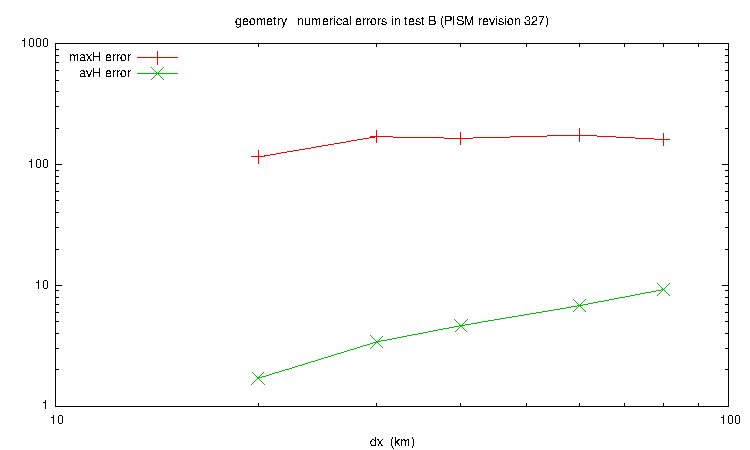
\includegraphics[width=4.8in,keepaspectratio=true]{figs/thickerrs_B}
\caption{Numerical thickness errors in test B.  Vertical axis is in meters. ``maxH error'' is the maximum thickness error anywhere on the grid, ``avH error'' is the average thickness error anywhere on the grid, and ``centerH error'' is the error at the center of the ice sheet.  See \cite{BLKCB} for discussion.}
\label{fig:thickerrsB}
\end{figure}

\begin{figure}[ht]
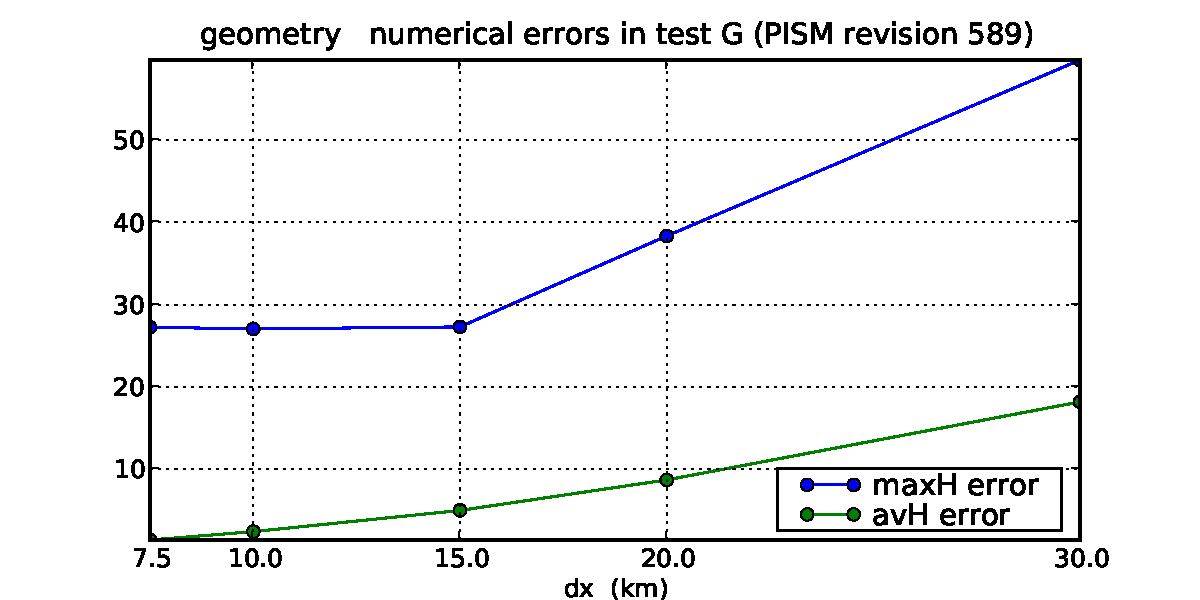
\includegraphics[width=4.8in,keepaspectratio=true]{figs/thickerrs_G}
\caption{Numerical thickness errors in test G.  Meaning exactly as in test C.  See \cite{BBL} and \cite{BLKCB} for discussion.}
\label{fig:thickerrsG}
\end{figure}

\begin{figure}[ht]
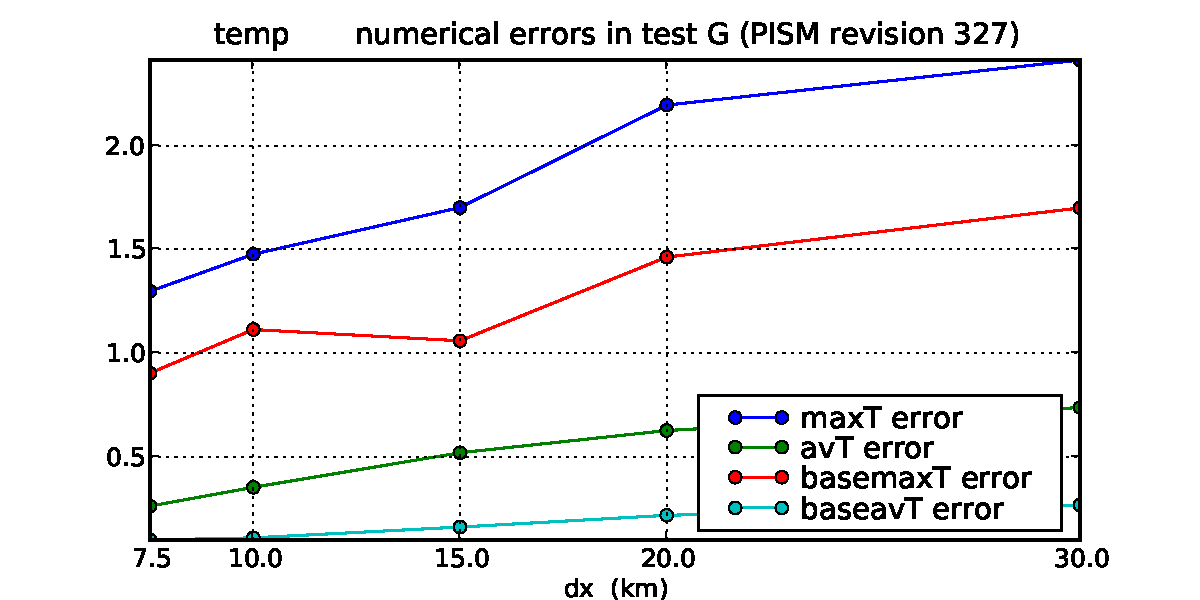
\includegraphics[width=4.8in,keepaspectratio=true]{figs/temperrs_G}
\caption{Numerical temperature errors in test G.  Vertical axis is in Kelvin.  ``maxT'' and ``basemaxT'' errors are maximum over all points within the ice and over all the basal points, respectively.  Similarly for ``avT'' and ``baseavT''; these are average errors.  See \cite{BBL} for discussion.}
\label{fig:temperrsG}
\end{figure}

\begin{figure}[ht]
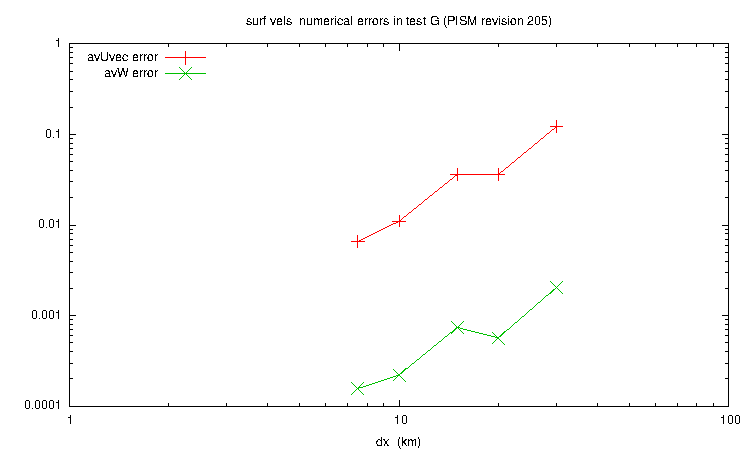
\includegraphics[width=4.8in,keepaspectratio=true]{figs/surfvelerrs_G}
\caption{Numerical errors in computed surface velocities in test G.  Vertical axis is in meters per year.}
\label{fig:surfvelerrsG}
\end{figure}

\begin{figure}[ht]
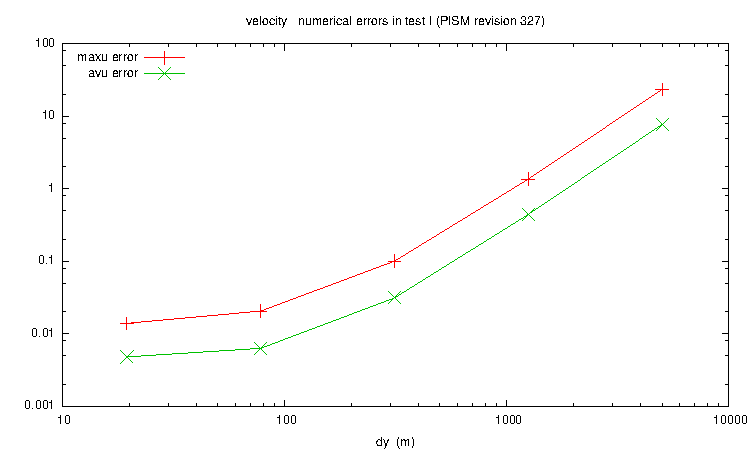
\includegraphics[width=4.8in,keepaspectratio=true]{figs/velerrs_I}
\caption{Numerical errors in horizontal velocities in test I, an ice stream.  Vertical axis is in meters per year.  See \cite{SchoofStream} for a description of the exact solution.}
\label{fig:velerrsI}
\end{figure}

\begin{figure}[ht]
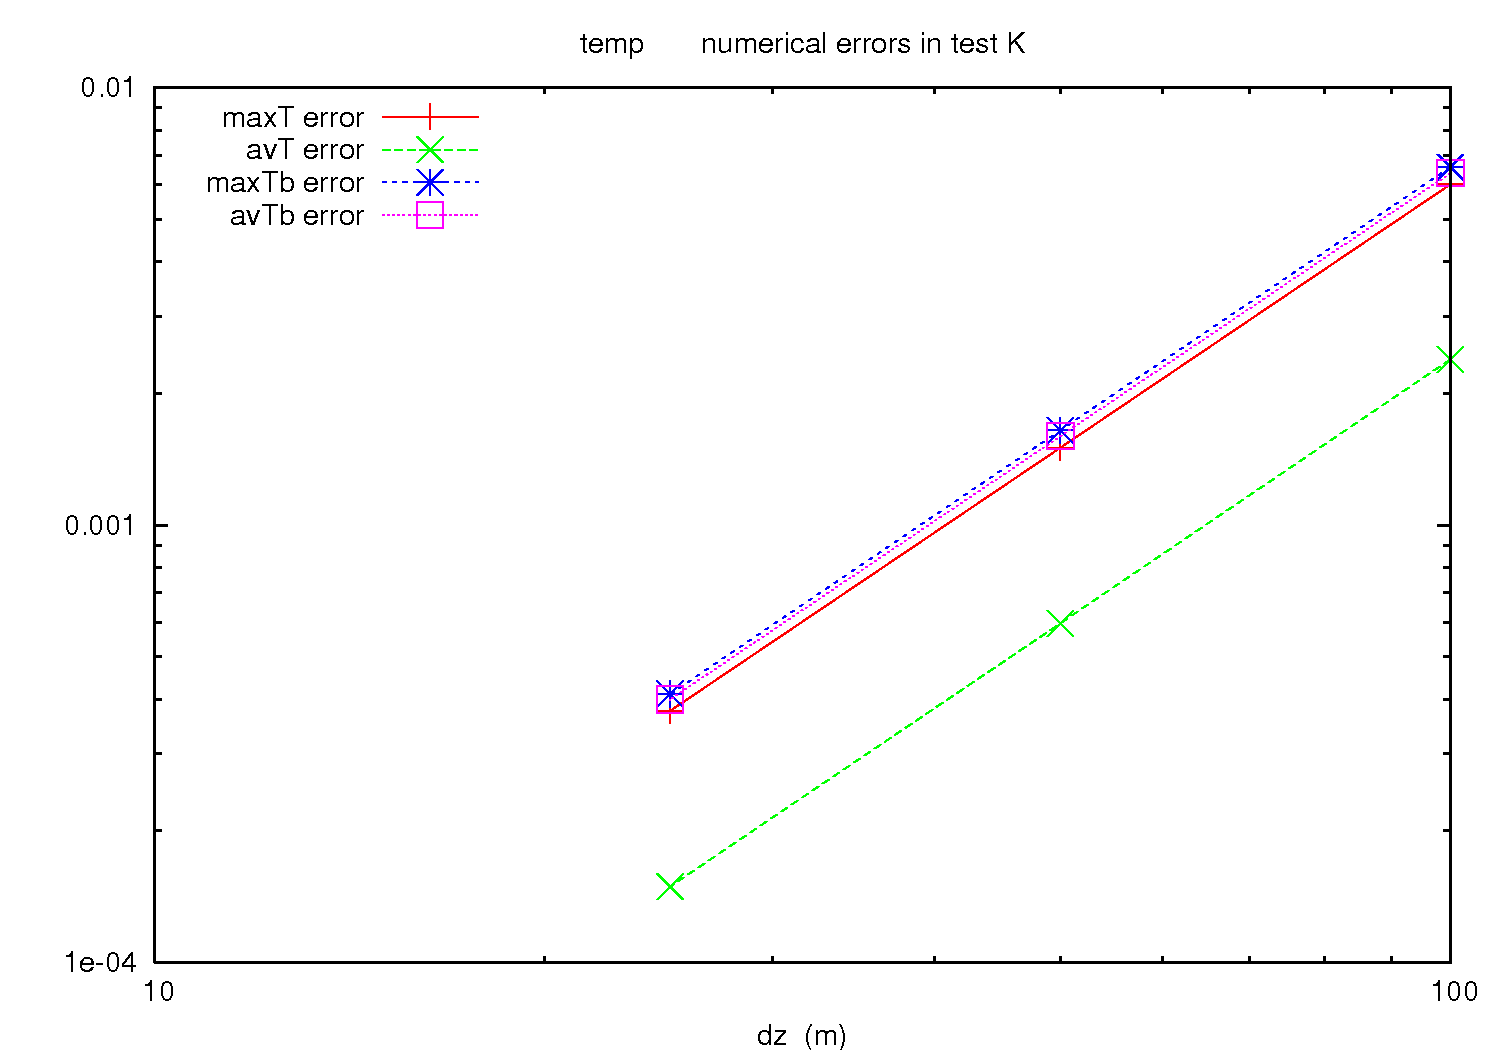
\includegraphics[width=4.8in,keepaspectratio=true]{figs/temperrs_K}
\caption{Numerical temperature errors in test K, which tests the thermal bedrock model.  Vertical axis is in Kelvin.  ``maxT'' and ``avT'' are errors computed over all points within the ice while ``maxTb'' and ``avTb'' are computed over all grid points within the bedrock.  See \cite{BuelerTestK} for a discussion.}
\label{fig:temperrsK}
\end{figure}


\clearpage\newpage
\section{Simplified geometry experiments}\label{sect:simp}

\subsection{Historical note}  There have been at least three stages of ice sheet model intercomparisons based on simplified geometry experiments since the early 1990s.

EISMINT I \cite{EISMINT96} was the first of these and involved only the isothermal shallow ice approximation (SIA).  (``EISMINT'' stands for European Ice Sheet Modeling INiTiative.)  Both fixed margin and moving margin experiments were performed in EISMINT I, and various conclusions were drawn about the several numerical schemes used in the intercomparison.  

EISMINT I is, however, superceded by \emph{verification} using the full variety of exact solutions to the isothermal SIA.  The reasons why EISMINT I can be fully replaced by verification are described in \cite{BLKCB}.  The ``rediscovery'', since EISMINT I, of the very useful Halfar similarity solution with zero accumulation \cite{Halfar83} is a particular reason why the ``moving margin'' experiment in EISMINT I is, roughly speaking, irrelevant.  For this reason there has been no attempt to support the EISMINT I experiments in PISM.

EISMINT II \cite{EISMINT00} was both a more significant and more controversial intercomparison.  It pointed out interesting and surprising properties of the thermocoupled SIA.  Here is not the place for a discussion of the interpretations which have followed the EISMINT II results, but references \cite{BBL,Hindmarsh04,Hindmarsh06,PayneBaldwin,SaitoEISMINT} each interpret the EISMINT II experiments and/or describe attempts to add more complete physical models to ``fix'' the perceived shortfalls of ice sheet models (as evidenced by their behavior on EISMINT II experiments).  PISM has built-in support for all of the published and unpublished EISMINT II experiments; these are described in the next subsection.

The ISMIP round of intercomparisons are ongoing at the time of this writing (2007); ``ISMIP'' stands for Ice Sheet Model Intercomparison Project.  At this time there are two components of ISMIP partially completed, namely HOM = Higher Order Models and HEINO = Heinrich Event INtercOmparison \cite{GreveTakahamaCalov}.

Of these ISMIP experiments, PISM currently only supports HEINO, but the results from PISM for HEINO are not regarded by the PISM authors as meaningful.  (ISMIP-HEINO support in PISM is an \emph{un}documented feature.)  We believe the continuum problem described by HEINO to not be easily approximate-able because of a (large) discontinuous jump in the basal velocity field.  This is a problem regardless of the details of the numerical schemes or even (roughly speaking) of the shallowness of the continuum model.

As of August 2007, the PISM developers plan to participate in the upcoming ISMIP-POLICE and Marine Ice Sheet Intercomparison exercises.

\subsection{EISMINT II in PISM}  There are seven experiments described in the published EISMINT II writeup \cite{EISMINT00}. They are labeled A, B, C, D, F, G, and H.  As specified in the writeup, the common features of all of these experiments are:\begin{itemize}
\item runs are of 200,000 years, with no prescribed time step;
\item runs are on a prescribed $61\times 61$ horizontal grid (but, as usual, the grid and the length of the run are command line options in PISM so PISM can easily run the same experiments on a refined grid);
\item the boundary conditions always have angular symmetry around the center of the grid;
\item the bed is always flat and does not move (so the effects of isostasy were ignored throughout);
\item the temperature in the bedrock is not modeled;
\item only shallow ice approximation physics is included;
\item the change in the temperature of ice is described by the shallow approximation of the conservation of energy \cite{Fowler};
\item thermomechanical coupling is included, both because of the temperature dependence of the softness of the ice, \emph{and} through the strain-heating (dissipation-heating) term in the conservation of energy equation;
\item the ice is \emph{cold} and not \emph{polythermal} \cite{Greve}; and finally
\item though basal melt rates may be computed diagnostically, they do not contribute to the dynamics of the ice sheet.
\end{itemize}
The experiments differ from each other in their various combinations of surface temperature and accumulation parameterizations.  Also, experiments H and G involve basal sliding, while the others don't.  Four experiments start with zero ice (A,F,G,H), while the other experiments (B,C,D) start from the final state of experiment A.

In addition to the seven experiments published in \cite{EISMINT00}, there were an additional five experiments described in the EISMINT II intercomparison description 
\cite{EISIIdescribe}, labeled E, I, J, K, and L.  These experiments share most features, itemized above, but with the following differences.  Experiment E is the same as experiment A except that the peak of the accumulation, and also the low point of the surface temperature, are shifted by 100 km in both $x$ and $y$ directions; also experiment E starts with the final state of experiment A.  Experiments I and J are similar to experiment A but with non-flat topography.  Experiments K and L are similar to experiment C but with non-flat topography.  See table \ref{tab:eisII} for how to run these experiments.

The vertical grid is not specified in the EISMINT II writeup.  It seems that good simulation of the complex thermomechanically coupled conditions near the base of the ice requires relatively fine resolution there.  Because PISM (currently) has an equally-spaced grid, we recommend the use of about 200 vertical levels.  Thus a reasonable experiment A run on one processor is

\verb|pisms -eisII A -Mx 61 -My 61 -Mz 201 -y 200000 -o eisIIA|

\noindent The final state \verb|eisIIA.nc| can, of course, be viewed using \verb|ncview|.

Table \ref{tab:eisII} shows how each of the EISMINT II experiments can be done in PISM.

\begin{table}[ht]
\caption{Running the EISMINT II experiments in PISM; the command is ``\t{pisms}'' plus the given options.}\label{tab:eisII}
\small
\begin{tabular}{@{}llll}\hline
\textbf{Command: ``\t{pisms}'' $+$} & \textbf{Relation to experiment A} \\ \hline
\verb|-eisII A -Mx 61 -My 61 -Mz 201 -y 2e5 -o eisIIA| & \\
\verb|-eisII B -if eisIIA.nc -y 2e5 -o eisIIB| & warmer \\
\verb|-eisII C -if eisIIA.nc -y 2e5 -o eisIIC| & less snow (lower accumulation)\\
\verb|-eisII D -if eisIIA.nc -y 2e5 -o eisIID| & only smaller area of accumulation \\
\verb|-eisII F -Mx 61 -My 61 -Mz 201 -y 200000 -o eisIIF| & colder; famous spokes \cite{BBL} \\
\verb|-eisII G -Mx 61 -My 61 -Mz 201 -y 200000 -o eisIIG| & sliding (regardless of temperature) \\
\verb|-eisII H -Mx 61 -My 61 -Mz 201 -y 200000 -o eisIIH| & melt-temperature activated sliding \\ \hline
\verb|-eisII E -if eisIIA.nc -y 2e5 -o eisIIE| & shifted accumulation/temperature maps \\
\verb|-eisII I -Mx 61 -My 61 -Mz 201 -y 2e5 -o eisIII| & trough topography \\
\verb|-eisII J -if eisIII -y 2e5 -o eisIIJ| & trough topography and less snow \\
\verb|-eisII K -Mx 61 -My 61 -Mz 201 -y 2e5 -o eisIIK| & mound topography \\
\verb|-eisII L -if eisIIK -y 2e5 -o eisIIL| & mound topography and less snow \\
\hline\normalsize
\end{tabular}\end{table}

The EISMINT II experiments can be run with various modifications of the default settings.  Of course the grid can be refined.  For instance, a twice as fine grid in the horizontal is ``\t{-Mx 121 -My 121}''.  Table \ref{tab:eisIIoptions} lists some optional settings which are particular to the EISMINT II experiments.  With the exception of ``\verb|-Lz|'', these options will only work if option ``\t{-eisII ?}'' is also set.

\begin{table}[ht]
\caption{Changing the default settings for the EISMINT II experiments in PISM.}\label{tab:eisIIoptions}
\small
\begin{tabular}{@{}llll}\hline
\textbf{Option} & \textbf{Default values [expers]} & \textbf{Units} & \textbf{Meaning} \\ \hline
\verb|-Mmax| & 0.5 [ABDEFGHIK], 0.25 [CJL] & m$/$a & max value of accumulation rate \\
\verb|-Rel| & 450 [ABEFGHIK], 425 [CDJL] & km & radial distance to equilibrium line \\
\verb|-Sb| & $10^{-2}$ [\emph{all}] & (m/a)/km & radial gradient of accumulation rate \\
\verb|-ST| & $1.67 \times 10^{-2}$ [\emph{all}] & K/km & radial gradient of surface temperature\\
\verb|-Tmin| & 238.15 [ACDEGHIJKL], & K & max of surface temperature \\
 & 243.15[B], 223.15[F] & & \\
\verb|-track_Hmelt| &  &  & compute effective thickness of basal melt \\
 &  &  & water (override default for EISMINT II) \\
\verb|-Lz| & 4500 [AE], 4000 [BCD], & m & height of the computational box \\
 & 5000 [F], 3000 [G] &  &  \\
\hline\normalsize
\end{tabular}\end{table}

Note that in PISM the height \verb|Lz| of the computational box is fixed at the beginning of the run.  On the other hand, changing the boundary conditions of the flow, as for instance by setting option \verb|-Mmax| to a larger than default value (see table \ref{tab:eisIIoptions}), may cause the ice sheet to thicken above the \verb|Lz| height.  If the ice grows above the height of the computational box then a ``\verb|Vertical grid exceeded!|'' or ``\verb|thickness overflow in SIA velocity: ks>Mz!|'' error occurs.  This can be fixed by remedied by restarting with a larger value for option \verb|-Lz|.


\begin{comment}
\subsection{ISMIP-HEINO in PISM}  The goal of the ISMIP-HEINO intercomparison is to evaluate the degree to which the thermomechanically coupled shallow ice approximation with basal sliding is a model for the surge behavior of the Laurentide ice sheet which is believed to have caused the ``Heinrich events'' described in [CITE HEINRICH].  Further information about HEINO, including the intercomparison description [URL FOR HEINO PDF] can be found at \url{http://www.pik-potsdam.de/~calov/heino.html}.

HEINO involves eight different runs of 200,000 years on a prescribed $81\times 81$ grid in the horizontal.  As in EISMINT II there is no prescription of vertical grid.  During the entirety of each run certain integrated quantities (area, melted base area, etc.) and other quantities measured at prescribed basal points must be reported at each year into ASCII files with \verb|.dat| extensions.  During the last 50,000 years of each of the eight runs, a map-plane (``planform'') dump of other quantities must be made to additional \verb|.dat| ASCII files.  These latter dumps must be made at the time of maximum and minimum extents of various quantities and the only way to determine the time of maximum/minimum extents is to complete the 200,000 year runs, determine the times of maximum and minimums, and then rerun the last 50,000 years from the saved state at 150,000 years.  See the intercomparison description [CITE URL for PDF].

PISM handles all the difficult details of the procedures described in the previous paragraph, but it is important for the user to have a sense for what is supposed to be reported.

HEINO is a relatively expensive intercomparison in terms of computer time.  For this reason use of a multiprocessor machine is recommended though not essential.  If the intercomparison participant's initials were X.~Y.~Z.~then a HEINO run ST is the recipe

\verb|mpiexec -n 8 pisms -ismip H -run ST -Mx 81 -My 81 -Mz 281 \|

\verb|    -y 150000 -dat_prefix XYZ_START -o XYZ_ST_150k|

\verb|mpiexec -n 8 pisms -ismip H -run ST -if XYZ_ST_150k.nc \|

\verb|    -y 50000 -dat_prefix XYZ_END -o XYZ_ST_200k|

[use Matlab to determine max/min]

\verb|mpiexec -n 8 pisms -ismip H -run ST -if XYZ_ST_150k.nc \|

\verb|    -y 50000 -time1 -time2 -time3 -time4 -dat_prefix XYZ_RERUN|

\verb|~/pism/test/heinocatdat.sh XYZ_ST_??? ...|

\verb|~/pism/test/renames.sh | [rename planform files?]

\noindent At the end of the above recipe the files [list] should appear.

\begin{table}[ht]
\caption{Options used in running ISMIP-HEINO in PISM.}\label{tab:heinooptions}
\small
\begin{tabular}{@{}llll}\hline
\textbf{Option} & \textbf{Default value(s)} & \textbf{Comments} \\ \hline
\verb|-| & & \\
\verb|-| & & \\
\verb|-dat_prefix| & \verb|PISM| & put initials here \\
\verb|-| & & \\
\verb|-ismip| & \verb|H| & only HEINO implemented for now \\
\verb|-| & & \\
\verb|-| & & \\
\verb|-| & & \\
\hline\normalsize
\end{tabular}\end{table}
\end{comment}




\clearpage\newpage
\section{Example: Modeling the Greenland ice sheet}\label{sect:green}  In this subsection we give an extended example of how to use PISM to model the Greenland ice sheet.  We use somewhat out-of-date data, namely data for the ice sheet modelling experiment (intercomparison) known as EISMINT-Greenland \cite{RitzEISMINT}.\footnote{Indeed the reader is encouraged to use PISM to build a better Greenland ice sheet model!}  Though based on old data, EISMINT-Greenland serves as an excellent tutorial example.  

As stated earlier, real data are not something we can freely distribute under the GNU Public License.  The data for performing this experiment are, however, freely available at
\medskip

\centerline{\protect{\textbf{\url{http://homepages.vub.ac.be/~phuybrec/eismint/greenland.html}}}}
\medskip

\noindent The snow-fall accumulation map, ablation parameterization, surface temperature formula, surface elevation, and bedrock elevation maps are essentially as in the 1991 papers \cite{Letreguillyetal1991,OhmuraReeh}.  Note that in the ice and sea floor-core driven ``forced climate'' run \verb|-ccl3| described below, the ice sheet is forced by changes in temperature from the GRIP core \cite{Dansgaardetal1993} and by changes in sea level from SPECMAP \cite{Imbrieetal1984}.  A parameter-sensitivity study of a EISMINT-Greenland type ice sheet model is described in \cite{RitzFabreLetreguilly}.

Substantial developments have occurred in modeling the Greenland ice sheet since the EISMINT-Greenland intercomparison.  For example, the relation between a Greenland ice sheet flow model, Earth deformation under ice sheet loads, and the reconstruction of global ice loading is analyzed in \cite{TarasovPeltier}.  The response of Greenland ice sheet models to climate warming is addressed in \cite{HuybrechtsdeWolde} and \cite{Greve00}.


\subsubsection*{Obtaining and converting EISMINT-Greenland data}  This subsection describes the use of two Python scripts to convert the EISMINT-Greenland data, which is in the form of several ASCII text files, into NetCDF files useable by PISM.

The Python scripts \verb|eis_green.py| and \verb|eis_core.py| can be found in the \verb|pism/test| directory.  In order to use the scripts, you must have downloaded the following ASCII files from the EISMINT-Greenland web site stated above:\begin{itemize}
 \item \verb|grid20-EISMINT|
 \item \verb|suaq20-EISMINT|
 \item \verb|specmap.017|
 \item \verb|sum89-92-ss09-50yr.stp|
\end{itemize}
The Python libraries \href{http://numpy.scipy.org/}{\texttt{numpy}} and \href{http://pysclint.sourceforge.net/pycdf/}{\texttt{pycdf}} must be present for our scripts to work.

Run

\verb|$ eis_green.py|

The NetCDF file \verb|eis_green20.nc| will be created from the data in \verb|grid20-EISMINT| and \verb|suaq20-EISMINT|.  It contains variables for the gridded latitude (\verb|lat|), longitude (\verb|lon|), surface altitude (\verb|h|), bedrock altitude (\verb|b|), and ice thickness (\verb|H|).  These values can be viewed graphically with \verb|ncview| (or as \emph{long} text files with \verb|ncdump|).

Note that the script \verb|eis_green.py| accepts option \verb|--prefix=foo/| to specify that the downloaded data is in directory \verb|foo/|.  (\verb|eis_core.py| below also takes this option.)  \verb|eis_green.py| also has option \verb|-g| to specify the grid spacing.  Use \verb|-g 40| if you downloaded \verb|grid40-EISMINT| and \verb|suaq40-EISMINT| 40 km data; use either \verb|-g 20| or no option to specify the 20 km data.

As an exercise, the \href{http://nco.sourceforge.net/}{\texttt{NCO}} can be used on \verb|eis_green20.nc| to compare the putative ice surface elevation to the sum of the ice thickness and the bed elevation:

\verb|$ ncap -O -vs "check=h-(H+b)" eis_green20.nc eis_green_check.nc|

\noindent The variable \verb|check| in the output file holds the difference of \verb|h| and the sum $\verb|b|+\verb|H|$.  Viewing \verb|check| in \verb|ncview| will show that \verb|h| is within 1 meter of $\verb|b|+\verb|H|$.  Thus the surface elevation \verb|h| is consistent.  It is also redundant: at bootstrapping, described below, PISM simply reads ice thickness \verb|H| and bed elevation \verb|b| and computes ice surface elevation as the sum of these two; the ice surface elevation variable \verb|h| is not actually read from the bootstrapping NetCDF file.

The bed elevation in the original data effectively contains a missing value attribute of $0.0$, because in several places---deep fjords, mostly---the observed bed elevation was not measured or the measured value was not trusted.  When viewing \verb|eis_green20.nc| with \verb|ncview|, these values show as white spots.  If these missing values are left in then the bed elevation map is extraordinarily rough and this makes reasonable ice flow predictions difficult.  We therefore suggest smoothing the bed elevations.  This can be done with another script named \verb|fill_missing.py|, found in directory \verb|pism/test/|. To use this script, the following command can be run:

\verb|$ fill_missing.py -i eis_green20.nc -v b -o eis_green_smoothed.nc|

\noindent Here, \verb|eis_green20.nc| is the input file, \verb|b| is the variable with missing values, and \verb|eis_green_|  \verb|smoothed.nc| is the output file. The script will look for an attribute named \verb|missing_value| and fill in the missing values according to the averages of its neighbors.  Multiple variables can be fixed at the same time by separating the variable names by commas.  (The script \verb|fill_missing.py| is a general tool for cleaning NetCDF files.  It is documented in Appendix D.)  

\begin{figure}[ht]
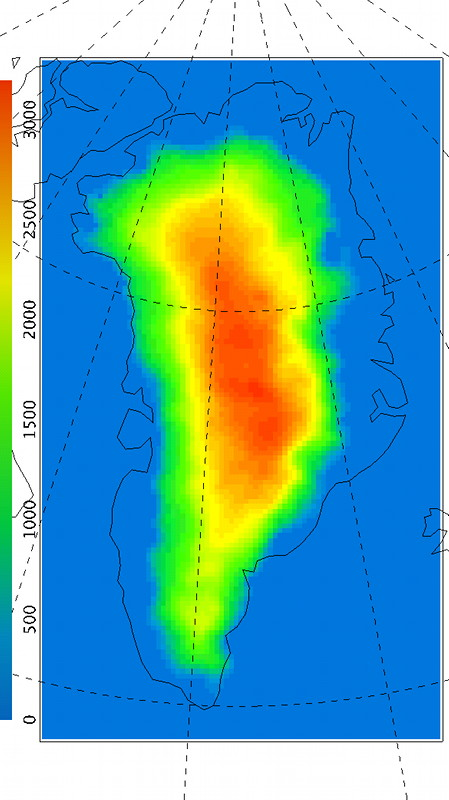
\includegraphics[width=2.8in,keepaspectratio=true]{figs/EISgreen_thick}\qquad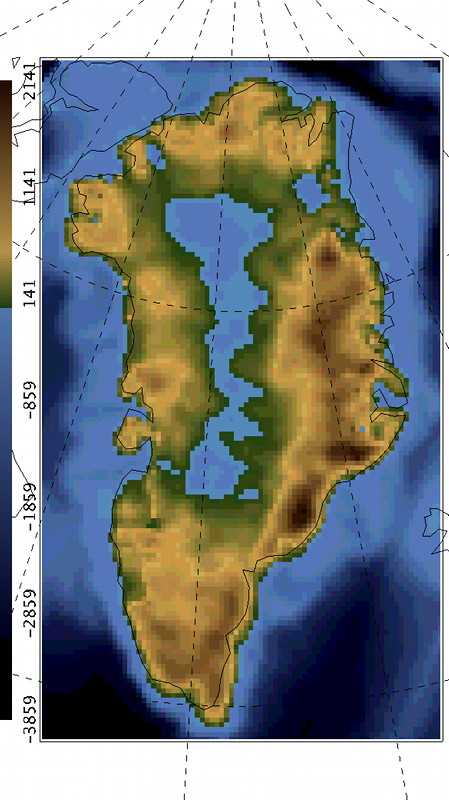
\includegraphics[width=3.0in,keepaspectratio=true]{figs/EISgreen_bed}
\caption{Views of the thickness (left) and smoothed bed elevation (right) for EISMINT-Greenland.  The coastal topography around several fjords has been smoothed.  These views are produced by \texttt{ncview} applied to \texttt{eis\und green \und smoothed.nc}.}
\label{fig:greendata}
\end{figure}

In addition to getting the EISMINT gridded data into NetCDF format and filling missing values, there is an issue with Ellesmere Island.  Ellesmere Island is very close to Greenland, and so it would be possible for the modeled ice sheet to flow onto to it.  (Indeed this presumably occurred at the last glacial maximum.)  Since we don't, however, have correct topography or accumulation rates for Ellesmere Island among the downloaded data, we want to prevent this from happening.  Therefore special code is executed by the relevant PISM executable \verb|pgrn| (see below).  It says that all points northwest of the line connecting the points $(68.18^\circ E, 80.1^\circ N)$ and $(62^\circ E, 82.24^\circ N)$ are removed from the flow simulation.  The same applies to anything east of $30^\circ E$ and south of $67^\circ N$ so that the flow could not spread to the tip of Iceland (not likely anyway \dots).  The phrase ``removed from the flow simulation'' actually means that the points are marked as ice-free ocean; note the use of option \verb|-ocean_kill| below.

We mentioned the script \verb|eis_core.py|.  Now we execute it:

\verb|$ eis_core.py|

\noindent If data files \verb|specmap.017| and \verb|sum89-92-ss09-50yr.stp| are not found in the current directory but instead in \verb|/foo/|, add the option \verb|--prefix=foo/|.

Two NetCDF files with one-dimensional (time series) data will be created, namely \verb|grip_dT.nc| and \verb|specmap_dSL.nc|.  Using \verb|ncview| on \verb|grip_dT.nc| gives the graph of temperature  shown in Figure \ref{fig:gripDeltaT}.

\begin{figure}[ht]
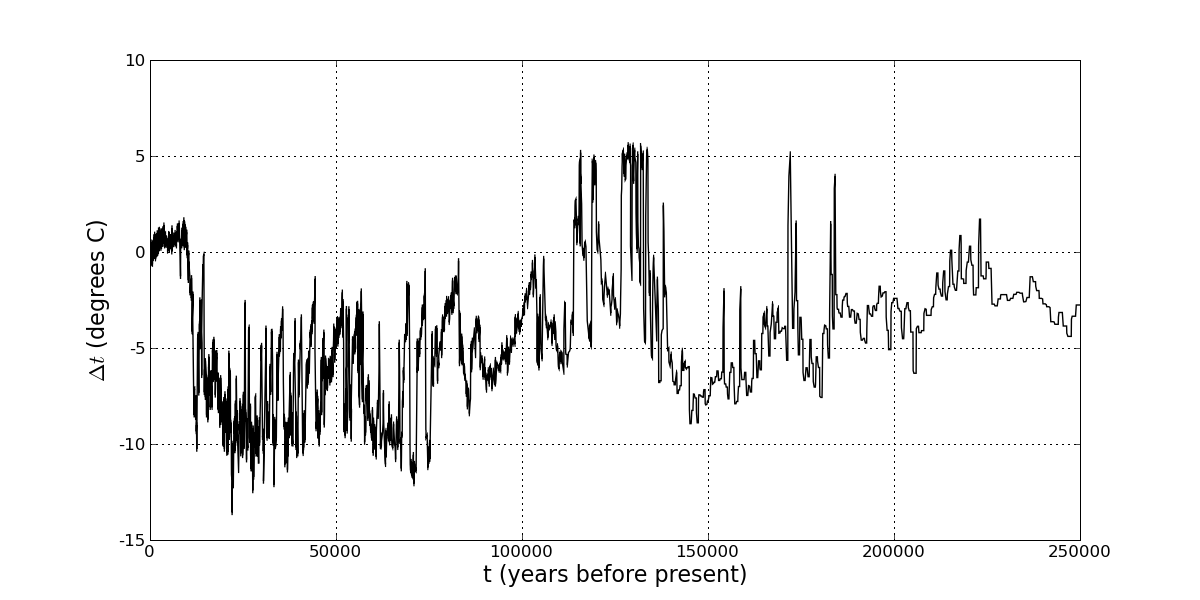
\includegraphics[width=5.6in,keepaspectratio=true]{figs/gripDeltaT}
\caption{Change in temperature from present, from the GRIP core.  A famous graph produced, in this case, by applying \texttt{ncview} to \texttt{grip\und dT.nc}}
\label{fig:gripDeltaT}
\end{figure}


\subsubsection*{Bootstrapping from EISMINT-Greenland data}  Once the EISMINT Greenland data is obtained and converted to NetCDF, as above, ``bootstrapping'' can begin.  By ``bootstrapping'' we mean the creation, by heuristics and simplified models, of the kind of full initial conditions needed for the continuum model (differential equations) inside PISM.\footnote{Section \ref{sect:boot} will explain, once written, that ``bootstrapping'' is a form of inverse modeling, and that we must inevitably do inverse modeling to do ice sheet modeling.}

The following one model year run is a basic version of ``bootstrapping''.  It is shown with \verb|-verbose| to suggest the many issues which arise.  Note that the EISMINT-Greenland specifies an 83 by 141 point grid, but you may use other numbers for \verb|-Mx| and \verb|-My| if desired.  Note that in PISM there is a uniform vertical grid.  Here, because the vertical dimension of the computational box is 4000 m, by specifying ``\verb|-Mz 201|'' we are choosing a 20 m spacing in the vertical.

\small\begin{quote}\begin{verbatim}
$ pgrn -bif eis_green_smoothed.nc -Mx 83 -My 141 -Mz 201 -y 1 -verbose -o green20km_y1
PGRN (EISMINT Greenland mode)
bootstrapping by PISM default method from file eis_green_smoothed.nc
  polar stereographic found: svlfp = -41.14, lopo =  71.65, sp =  71.00
  time t found in bootstrap file; using to set current year
  using default value Lz=4000.000000 for vertical extent of computational box for ice
  WARNING: ignoring values found for surface elevation h and using h = b + H
  WARNING: surface temperature Ts not found; using default  263.15 K
  WARNING: geothermal flux ghf not found; using default  0.042 W/m^2
  uplift not found. Filling with zero
  Hmelt not found. Filling with zero
  done reading .nc file
  determining mask by floating criterion; grounded ice marked as SIA (=1)
  setting accumulation in ice shelf-free ocean to default value -20.00 m/a
  filling in temperatures at depth using surface temperatures and quartic guess
bootstrapping by PISM default method done
geothermal flux set to EISMINT-Greenland value 0.050000 W/m^2
computing surface temperatures according to EISMINT-Greenland rule 
   (uses surface elevation and latitude)
filling in temperatures at depth using surface temperatures and quartic guess
removing extra land (Ellesmere Island and Iceland) using EISMINT-Greenland rule
  [computational box for ice: ( 1640.00 km) x ( 2800.00 km) x ( 4000.00 m)]
  [grid cell dimensions     : (   20.00 km) x (   20.00 km) x (   20.00 m)]
  IceParam: Mx = 83, My = 141, Mz = 201, Mbz = 1,
            Lx = 820.00 km, Ly = 1400.00 m, Lz = 4000.00 m, Lbz =   0.00 m,
            dx = 20.000 km, dy = 20.000 km, dz = 20.000 m, year =   0.0000,
.
.
.
Writing model state to file `green20km_y1.nc' ... done.
\end{verbatim}
\end{quote}\normalsize

\noindent Let's explain what has happened.  The EISMINT-Greenland data, as with \emph{all} real ice sheet data, does not contain certain variables necessary to initialize PISM in the sense of initial values for the relevant partial differential equations.  For instance, the data do not include the temperature of the ice anywhere but at the surface.  The data also do not include the amount of water stored in the till, for instance.  So PISM fills in the unknown initial conditions based on some default guesses; this is the section above bracketed by \verb|bootstrapping by PISM default method|\dots and \verb|bootstrapping| \verb|by PISM default| \verb|method done|. 

The option ``\verb|-bif|'' stands for ``bootstrapping input file''.  (This option is an alternative to ``\verb|-if|'', standing for ``input file'', which is used for a file which has full initial conditions.  In practice, ``\verb|-if|'' is only used with a NetCDF file which was previously saved by PISM.)

Regarding the temperature within the ice, bootstrapping applies an interpolation scheme to the surface temperatures and geothermal fluxes.  It is based on a heuristic for the amount of downward flow in a column, to create a temperature field at depth.  %See the Reference Manual.

In fact this bootstrapping mode fills in several default values.  For instance, the variables \verb|ghf|, \verb|uplift|, and \verb|Hmelt| were not found in the \verb|-bif| file, whereas they would be in a saved PISM model state (which would be loaded with option \verb|-if|).  Thus, these variables were filled with defaults \verb|0.042| $\text{mW}/\text{m}^2$, \verb|0| $\text{m}/\text{s}$, and \verb|0| m respectively.  Also, recall that the EISMINT Greenland data had redundant surface elevation (\verb|h|) values.  We see that in PISM's default bootstrapping the variable \verb|h| is ignored and PISM uses the sum of bed elevation and ice thickness ``\verb|h = b + H|''.

Continuing with the above output, after default bootstrapping there are additional settings special to EISMINT-Greenland.  For instance, at the surface there is a formula which determines the temperature as a function of altitude and latitude.  (There is no EISMINT-Greenland gridded data set for surface temperature; see \cite{RitzEISMINT}.)  The executable \verb|pgrn| knows this formula and uses it.  Also, the constant value for geothermal flux is reset, and the Ellesmere Island issue is resolved.

Before seeking a good steady state for the entire thermomechanically-coupled ice sheet, it is helpful to do a better job of filling the temperatures within the ice than has already been done.  One way to do this is to have the temperature field and velocity field co-evolve according to the thermomechanical flow model, but while holding the (free) ice surface stationary.  This is a continuation of the ``bootstrapping'' idea, because the effect is to replace the heuristic temperature field applied above by one which includes horizontal advection.  The resulting temperature field is still not the fully physical temperature field because it comes from a steadiness assumption about position of the surface of the ice.

We create this temperature field by running for 10000 years with non-evolving surface, using the option \verb|-no_mass| to turn off the map-plane mass continuity scheme:

\verb|$ mpiexec -n 2 pgrn -if green20km_y1.nc -no_mass -y 10000 -o green20km_Tsteady|

\noindent This last run takes a significant amount of computer time (at least several hours).  In fact it should probably be done longer for serious modeling because the exponential time constant for decay of the thermomechanically-coupled system toward equilibrium is probably about 100k years (or perhaps even more).

This is a case where many more processors \emph{are} effective, up to perhaps 40 to 80 processors for the 83 by 141 grid.  (Finer grids allow good parallel performance for more processors.)

Because of the current PISM implementation of the positive degree day model specified by EISMINT-Greenland, the time steps are of at most one model year.  (This is one of several efficiency issues which should be resolved in the future; note reference \cite{CalovGreve05}.)

\subsubsection*{Running the EISMINT-Greenland steady state experiments}  Now that we have initial conditions including a vaguely-credible temperature field, our first experiment is the steady state run ``SSL2''.  This experiment uses the parameters specified in the EISMINT-Greenland description \cite{RitzEISMINT}.  This run is intended to go until the model reaches a ``steady state'', a phrase which \cite{RitzEISMINT} defines to mean a particular standard for a small volume change rate (less than a .01\% change in volume in 10,000 years).

The PISM distribution includes a script that automates the process of checking the steady state condition.  Thus it is not necessary to manually check the changes in volume.  This script is called \verb|ssl_exper.py| and is in the \verb|pism/test| directory.  When run it will save states every 10,000 years (or other chosen interval), until the change in volume between saved states is less than a specified criterion.  It uses the \href{http://nco.sourceforge.net/}{NCO} to compare the thicknesses in saved model states.  It can be used with multiple processors by setting the option \verb|-n|; see Appendix D for documentation of the options.

For illustration we do:

\verb|$  ssl_exper.py -n 8 -i green20km_Tsteady.nc -t 1 -c 0.01|

\noindent Here we specify that the criterion for steady state is weak so that our example takes less computer time; we ask for less than 1\% change (``\verb|-c 0.01|'') between 1000 year runs (``\verb|-t 1|'').  With 8 processors this example completes in several hours.  The actual EISMINT-Greenland run would be

\verb|$  ssl_exper.py -n 8 -i green20km_Tsteady.nc -t 10 -c 0.0001|

(With 80 processors this full run completed in 5 hours.  Efficiency is a concern for PISM, but functionality and correctness are coming first \dots)  

The example run gives this output:

\small\begin{quote}\begin{verbatim}
$ ssl_exper.py -n 8 -i green20km_Tsteady.nc -t 1 -c 0.01
  [using 8 processors]
  [using interval of 1k years between volume measurements]
  [using criterion of 1.0 percent change between volume measurements]
  running from 0k years until 1k years ...
  trying:  mpiexec -n 8 pgrn -ssl2 -if green20km_Tsteady.nc -y 1000 -ys 0 -ocean_kill
     -tempskip 3 -o green_SSL2_1k >> out.txt
  sum of H for 0k, 1k years, resp.: 7063322.500000, 8002617.500000
  volume change is: 11.7373471867%
  running from 1k years until 2k years ...
  trying:  mpiexec -n 8 pgrn -ssl2 -if green_SSL2_1k.nc -y 1000 -ocean_kill
     -tempskip 3 -o green_SSL2_2k >> out.txt
  sum of H for 1k, 2k years, resp.: 8002617.500000, 8598249.000000
  volume change is: 6.92735811675%
  running from 2k years until 3k years ...
.
.
.
  running from 7k years until 8k years ...
  trying:  mpiexec -n 8 pgrn -ssl2 -if green_SSL2_7k.nc -y 1000 -ocean_kill
     -tempskip 3 -o green_SSL2_8k >> out.txt
  sum of H for 7k, 8k years, resp.: 9836617.000000, 9915852.000000
  volume change is: 0.799074048302%
  resulting volume change below criterion; ending
\end{verbatim}
\end{quote}\normalsize

We see that the volume gradually increases but does settle down.  Inspection of the standard output of the run (e.g.~\verb|less out.txt|) shows that the initial volume of $2.825 \times 10^{6}\,\text{km}^3$ grows to $3.966 \times 10^{6}\,\text{km}^3$ at $8000$ model years.  In fact, to see the behavior over time of the volume, area, basal melt fraction, and so on, use the Python script \verb|test/series.py| documented in Appendix D:

\verb|$  series.py -f out.txt -o illust_series.nc|

\noindent Then view the time series using \verb|ncview|, for instance.  One sees that the volume shows a consistent growing-but-leveling-out trend, with a final volume expected to be a bit more than $4 \times 10^{6}\,\text{km}^3$.

In fact that is what happens.  If we run the SSL2 experiment with the specified ``0.01\% change in 10k years'' criterion, then the run ends at 110k years with a volume change of about 0.001\% between the 100k and 110k model states.  The final volume was $4.087 \times 10^{6}\,\text{km}^3$.  The time series for volume and melt fraction (the fraction of the base where the temperature is at pressure-melting) are shown in Figures \ref{fig:eisgrnvolseries} and \ref{fig:eisgrnmeltfseries}.  The volume time series is boring, but the melt fraction indicates something interesting: measured by basal melt fraction, the temperature field resulting from bootstrapping (above) was a very reasonable guess.

\begin{figure}[ht]
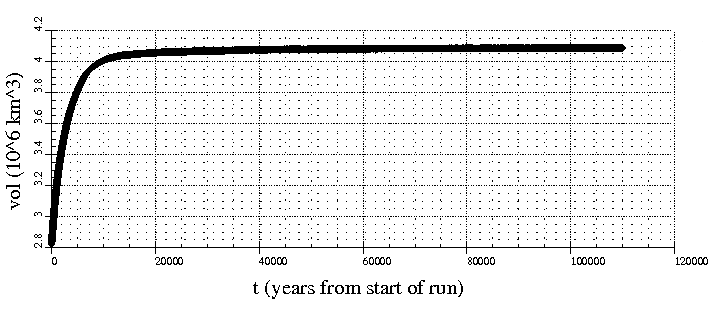
\includegraphics[width=6.0in,keepaspectratio=true]{figs/eisgrn_volseries}
\caption{Volume time series for a 110k model year EISMINT-Greenland run; units of $10^{6}\,\text{km}^3$.}
\label{fig:eisgrnvolseries}
\end{figure}

\begin{figure}[ht]
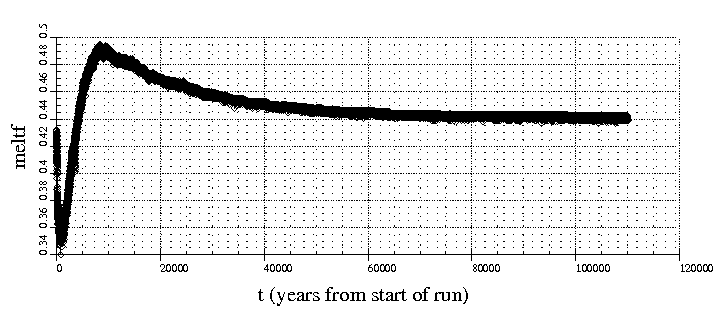
\includegraphics[width=6.0in,keepaspectratio=true]{figs/eisgrn_meltfseries}
\caption{Time series for the fraction of the base which is at the pressure-melting temperature from a 110k model year EISMINT-Greenland run.  See the right hand part of Figure \ref{fig:ssl2thickThomol} for a map of the basal temperature.}
\label{fig:eisgrnmeltfseries}
\end{figure}

The final saved state is called \verb| green_SSL2_110k.nc|; we will use this NetCDF file to continue the EISMINT-Greenland experiments below.  The saved ice thickness and homologous basal temperature maps are shown in Figure \ref{fig:ssl2thickThomol}.  The vertically-averaged horizontal velocity is shown in Figure \ref{fig:ssl2cbar}.  

\begin{figure}[ht]
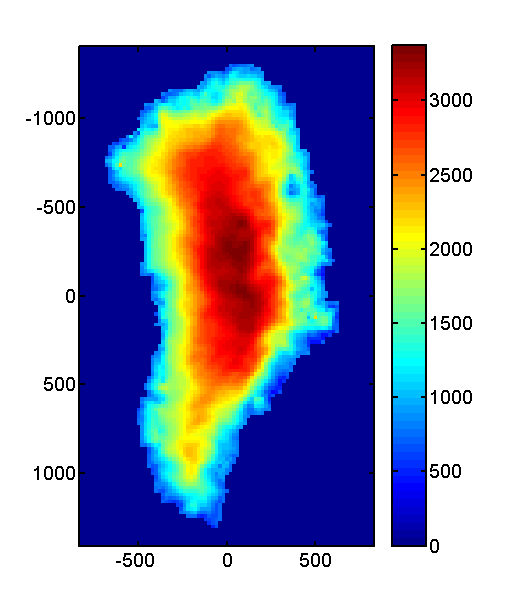
\includegraphics[height=3.7in,keepaspectratio=true]{figs/greenH_SSL2}\qquad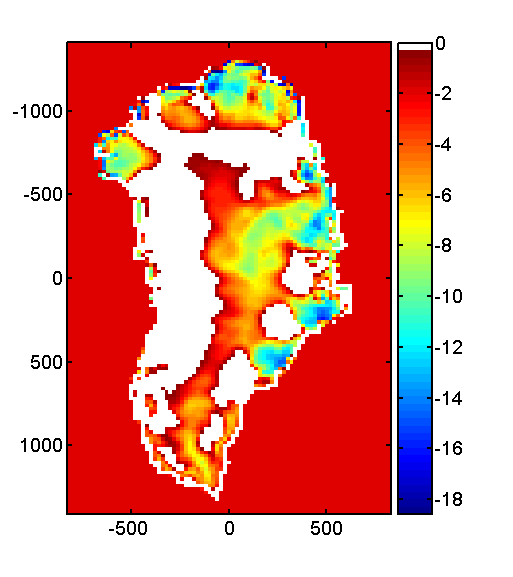
\includegraphics[height=3.7in,width=2.9in]{figs/greenThomol_SSL2}
\caption{Ice thickness (meters; left) and homologous basal temperature (degrees C below 0; right) at the end (110k model years) of a EISMINT-Greenland SSL2 run.  Note that in the temperature graph the pressure-melting temperature areas are white.}
\label{fig:ssl2thickThomol}
\end{figure}

\begin{figure}[ht]
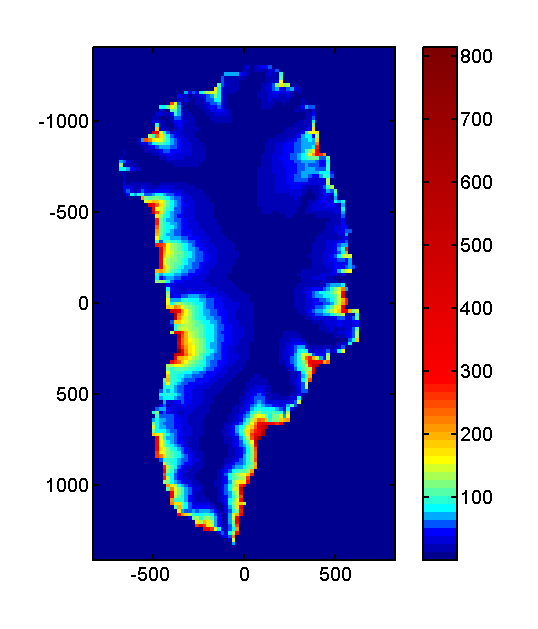
\includegraphics[height=3.9in,keepaspectratio=true]{figs/greencbar_SSL2}
\caption{Vertically-averaged horizontal velocity in meters per year at the end (110k model years) of a EISMINT-Greenland SSL2 run.}
\label{fig:ssl2cbar}
\end{figure}

One may also give a \verb|--ssl3| option to \verb|ssl_exper.py| to run an EISMINT-Greenland ``SSL3'' experiment \cite{RitzEISMINT}.  (Giving this option to \verb|ssl_exper.py| actually gives a \verb|-ssl3 -gk| option to \verb|pgrn|.)  The PISM interpretation of the SSL3 experiment happens to be: \begin{itemize}
\item use Goldsby-Kohlstedt flow law \cite{GoldsbyKohlstedt} with an enhancement factor of 1.0, and
\item allow pressure-melting temperature dependent linear sliding with a sliding coefficient that gives 50 m/a sliding at 100 kPa (1 bar).
\end{itemize}
There is no assertion that these are superior modeling choices.  We give ``SSL3'' this interpretation merely for illustration.  Note that because of the basal sliding, with sliding velocity proportional to the driving shear stress at the base, the volume time series never quite settles down (not shown).

\subsubsection*{Climate forcing from GRIP and SPECMAP}  The next experiment is intended to be carried out after the completion of the steady state run above.

Recall that the NetCDF files \verb|grip_dT.nc| and \verb|specmap_dSL.nc| contain time series data for change in surface temperature and the change in sea level.  The options \verb|-dTforcing| and \verb|-dSLforcing| for \verb|pgrn| can use these data for a ``CCL3'' run \cite{RitzEISMINT} under PISM.  Before every time step, \verb|pgrn| adds in a change to the surface temperature and sea level in order to incorporate the effects of global climate changes.  The data in \verb|grip_dT.nc| goes about 250,000 years into the past, while the data in \verb|specmap_dSL.nc| goes back about 780,000 years, but EISMINT-Greenland specifies that the run will start at the beginning of the GRIP data.  Thus we manually set the starting year using the option \verb|-ys|.  The CCL3 experiment can be run using the following command:\footnote{Actually this is in error relative to the EISMINT-Greenland description \cite{RitzEISMINT,HuybrechtsEISMINT}.  In particular, ``isostatic response should be modelled also''.  Also it should be with SSL3 parameterizations.  Thus the run should really add the options \texttt{-bed\und def\und lc -gk}.  Such a run would have the bed deformation (here modelled using the methods in \cite{BLKfastearth,LingleClark}) affect the sea level and thus the boundary condition of the ice sheet.}

\verb|$  pgrn -ccl3 -if green_SSL2_110k.nc -dTforcing grip_dT.nc \|

\verb|      -dSLforcing specmap_dSL.nc -ys -249900 -ye 0 -o green_CCL3_y0|

The resulting thickness difference, relative to the end of the SSL2 run, and the homologous basal temperature, are shown in Figure \ref{fig:cclthickThomol}.

\begin{figure}[ht]
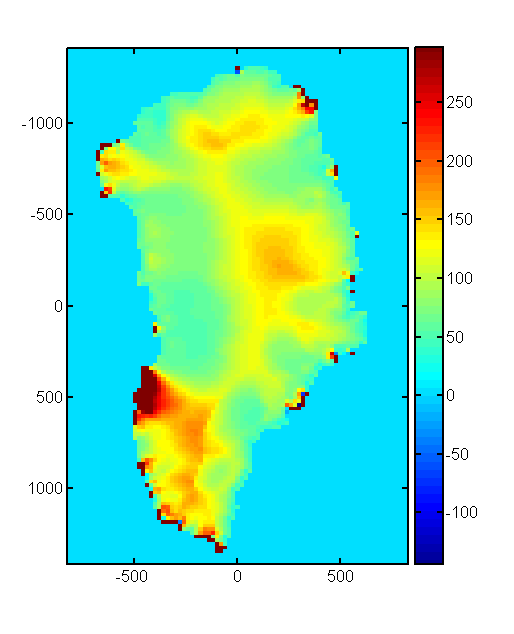
\includegraphics[height=3.7in,keepaspectratio=true]{figs/Hdiff_CCLSSL}\qquad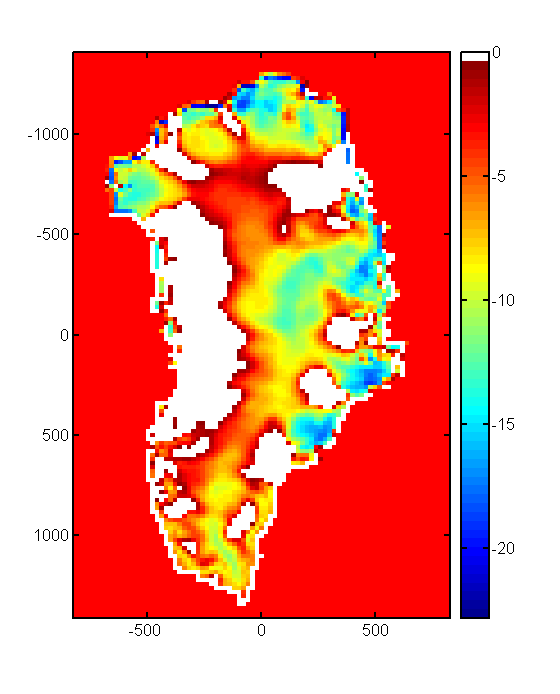
\includegraphics[height=3.7in,width=2.9in]{figs/Thomol_CCL}
\caption{Left:  Ice thickness difference between end (year zero) of a CCL3 run and the end of an SSL2 run (meters).  Right:  Ice homologous basal temperature (degrees C below 0; right) at the end of a EISMINT-Greenland CCL3 run.  Compare Figure \ref{fig:ssl2thickThomol}.}
\label{fig:cclthickThomol}
\end{figure}

EISMINT-Greenland also calls for a baseline run for another 500 years which starts from the end of the CCL3 run and has steady current climate forcing.  If \verb|pgrn -ccl3| is run past year 0, and thus past the end of the GRIP and SPECMAP data, this baseline run will occur by default.  So the previous command can be run for another 500 years, and the forcing can be omitted:

\verb|$  pgrn -ccl3 -if green_CCL3_y0.nc -y 500 -o green_CCL3_y500|

\subsubsection*{A greenhouse warming scenario}  A final ``greenhouse warming'' experiment ``GWL3'' is described in the EISMINT-Greenland \cite{RitzEISMINT}.  It uses the model state obtained for present day from the CCL3 run.  The GWL3 experiment (option \verb|-gwl3|) runs for 500 years with the temperature increasing by $0.035^\circ C/$year for the first 80 years, then at a rate of $0.0017^\circ C/$year for the last 420 years:

\verb|$  pgrn -gwl3 -if green_CCL3_y0.nc -y 500 -o green_GWL3_y500|



\clearpage\newpage
\section{Example: Validating PISM as a flow model for the Ross ice shelf}\label{sect:ross}  Recall that we use the term ``validation'' to describe the comparison of model output with physical observations in cases where those physical observations are believed to be sufficiently complete and of sufficient quality so that the performance of the numerical model can be assessed.  Roughly speaking, in validation the observations or data are better than the model, so the comparison tells one about the quality of the model and not the quality or incompleteness of the data.

As part of the first EISMINT series of intercomparisons, MacAyeal and others \cite{MacAyealetal} performed a validation of several ice shelf numerical models using the Ross ice shelf as an example.  We will refer to this intercomparison and its associate write-up \cite{MacAyealetal} as ``EISMINT-Ross''.  The models were compared to data from the RIGGS (= Ross Ice shelf Geophysical and Glaciological Survey) \cite{RIGGS1,RIGGS2}.  The RIGGS data were acquired in the period 1973--1978.   In particular, the RIGGS data include the (horizontal) velocity of the ice shelf measured at a few hundred locations in a reasonably regular grid across the shelf; see figure \ref{fig:rossmatlab} below for an indicaiton of these positions.

Substantial developments have occurred in the modeling of the Ross ice shelf since the EISMINT-Ross intercomparison.  For example, inverse modeling techniques were used to recover depth-averaged viscosity of the Ross ice shelf from the RIGGS data \cite{RommelaereMacAyeal} and a parameter-sensitivity study was performed for a particular Ross ice shelf numerical model \cite{HumbertGreveHutter}. 

\subsubsection*{Bringing in the data}  Using these data to validate PISM's ice shelf modeling abilities requires downloading (text) data files from the website \url{http://homepages.vub.ac.be/~phuybrec/eismint/iceshelf.html}.  In particular, these files must be downloaded:
\begin{itemize}
\item \verb|111by147Grid.dat|
\item \verb|kbc.dat|
\item \verb|inlets.dat|
\end{itemize}
In the next step we will assume that these three files are in a directory \verb|eisDownload/|, and we will refer to these as the ``EISMINT-Ross'' data.  Note that these data are for a particular rectangular grid with $6.822$km spacing in both $x$ and $y$ directions, but that (as usual) the PISM computational grid is determined by the user.

The first step for using these data, as usual for PISM, is to convert them to a machine readable NetCDF file.  There is already a script \verb|eis_ross.py| for this purpose in subdirectory \verb|pism/test/ross/|.  It  reads the above three EISMINT-Ross \verb|.dat| files and it creates a NetCDF file with the data and some metadate needed by PISM.  It is used this way:

\verb|test/ross/eis_ross.py --prefix=eisDownload/ -o ross.nc|

\noindent The output file can be reconverted to text (CDL) using \verb|ncdump| or it can be viewed graphically with \verb|ncview|.

\begin{figure}[ht]
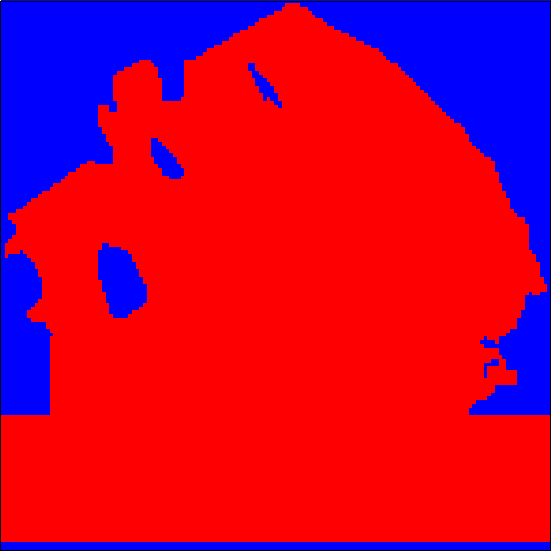
\includegraphics[height=2.3in,keepaspectratio=true]{figs/rossmask} \qquad 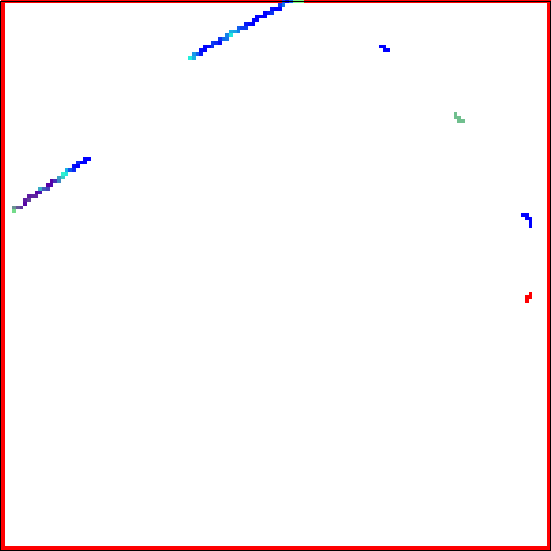
\includegraphics[height=2.3in,keepaspectratio=true]{figs/rossubar}
\caption{Two views from \protect{\texttt{ncview}} of the EISMINT-Ross data in the NetCDF file \protect{\texttt{ross.nc}}.  The floating-versus-grounded mask (left; red areas are floating ice shelf) and the $x$-component of the non-zero kinematic (Dirichlet) boundary condition for velocity (right).}
\label{fig:rossmaskubar}
\end{figure}

The NetCDF file \verb|ross.nc| contains ice thickness, bed elevations, surface temperature, and accumulation, and all of these are typical of ice sheet modeling data.  It also has variables \verb|ubar| and \verb|vbar| which give the boundary values which are needed for the diagnostic computation of velocity.  Also present are the variables \verb|mask|, which shows the domain where the ice shelf is modeled, and \verb|bcflag|, which shows the locations where the boundary conditions are to be applied.  Note that the original EISMINT-Ross data are on a 111 by 147 grid but that \verb|eis_ross.py| extends this grid to a more convenient 147 by 147 grid, with the same $6.822$km spacing, which has ice-free ocean beyond the (straightened; compare \cite{MacAyealetal}) calving front.  See figure \ref{fig:rossmaskubar}.

\subsubsection*{Diagnostic computation of ice shelf velocity}  The basic Ross ice shelf velocity computation from these data might be:

\verb|   pismd -ross -bif ross.nc -ssaBC ross.nc -Mx 147 -My 147 -Mz 11 -mv|

\noindent Here we bootstrap (\verb|-bif|) from \verb|ross.nc|.  We also use option \verb|-ssaBC| to specify \verb|ross.nc| as the source of the boundary value data for the ice shelf equations, as mentioned in the last paragraph.  The computational grid specified here is the $6.822$ km data grid in EISMINT-Ross with 147 grid points in each direction.  Note that the small number of vertical levels (\verb|-Mz 11|) is reasonable because the EISMINT-Ross intercomparison specifies that the temperature at depth be the surface temperature \cite{MacAyealetal}, and thus there is no thermocoupling issue.

At the end of this run the computed velocity field is compared to the interpolated data on observed velocities in the file \verb|ross.nc|.  (In particular, that NetCDF file contains a variable \verb|accur| which identifies the region in which the observed velocities are valid.  The observed (interpolated) velocities themselves are stored in variables \verb|mag_obs| and \verb|azi_obs|.)  We see that the largest computed velocity in the ice shelf is just under a thousand meters per year, and that errors in the vector values of velocity are roughly 10\% in a sum of squares average sense.  (There is more on viewing the results, on measuring the correspondence with measurements, and on tuning the hardness parameter to fit the data, below.)

There are many variations on this basic ``\verb|pismd -ross|'' run above.  First of all one can get more information during the run by adding diagnositic viewers and a more complete (verbose) report to standard out:

\verb|   pismd -ross -bif ross.nc -ssaBC ross.nc -Mx 147 -My 147 -Mz 11 -mv \|

\verb|     -d cnmu -verbose 4 -pause 10|

\noindent Secondly one might want to do the run in parallel, do it on a finer grid, and ask for higher tolerance.  For example, 

\small
\verb|   mpiexec -n 6 pismd -ross -bif ross.nc -ssaBC ross.nc -Mx 201 -My 201 -Mz 11 -mv|
\normalsize

The result is not exactly the same [but really good; FIXME].

Alternately one might want to change the hardness parameter from the default value $\bar B = 1.9 \times 10^8 \, \text{Pa}\, \text{s}^{1/3}$ \cite{MacAyealetal} to a slightly softer value because the highest computed velocity with the default setting is a little lower than the maximum measured in the RIGGS data (namely, $1007$ m/a; see files \verb|pism/test/ross/README| and \verb|pism/test/ross/riggs_clean.dat|).   We can also use lower (more severe) tolerances for the nonlinear iteration (\verb|-mv_rtol|) and the linear iteration (\verb|-ksp_rtol|) to get more confidence in the numerical scheme.   Finally we can also save the model state with a meaningful name:

\verb|   pismd -ross -bif ross.nc -ssaBC ross.nc -Mx 147 -My 147 -Mz 11 -mv \|

\verb|     -verbose 4 -constant_hardness 1.8e8 -mv_rtol 1e-6 -ksp_rtol 1e-10 \|

\verb|     -o ross_out_1p8|

\noindent Using \verb|ncview| on \verb|ross_out_1p8.nc| to view the horizontal speed of the ice shelf gives figure \ref{fig:rossspeed1p8}.

\begin{figure}[ht]
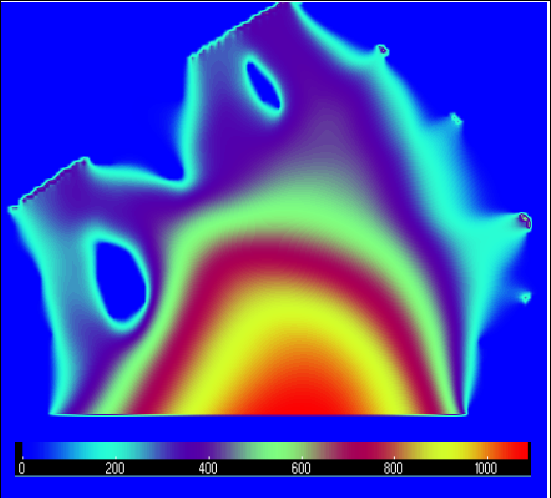
\includegraphics[height=3.5in,keepaspectratio=true]{figs/rossspeed1p8}
\caption{Computed horizontal speed of the Ross ice shelf using $\bar B = 1.8 \times 10^8 \, \text{Pa}\, \text{s}^{1/3}$.  Color gives velocity in m/a; see scale.}
\label{fig:rossspeed1p8}
\end{figure}

\small
\begin{table}[ht]
\caption{Non-obvious options available and/or recommended with \texttt{pismd -ross}.}\label{tab:rossoptions}
\begin{tabular}{@{}llll}\hline
\textbf{Option} & \textbf{Explanation/Comments} \\ \hline
  \verb|-d cnmu| &       a good way to see what is going on \\
  \verb|-o foo -of nm| &  writes NetCDF file \verb|foo.nc| with full three-dimensional \\
    & velocity fields \emph{and} writes some model results to \\
    & Matlab-readable file \verb|foo.m| \\
  \verb|-pause N| &      pause for N seconds when refreshing viewers \\
  \verb|-ross| &         only use with executable \verb|pismd| \\
  \verb|-tune x,y,z| &   run through constant hardness values $\bar B = x, x+y, x+2y,$ \\
 & $\dots, z(=x+ky)$; (note no spaces in ``\verb|x,y,z|'') \\
  \verb|-verbose 4| &      shows information on nonlinear iteration and Krylov solve \\
    & and parameters related to solving the ice shelf equations \\
\hline
\end{tabular}
\end{table}
\normalsize

Table \ref{tab:rossoptions} lists some of the options which are useful for this kind of diagnositic velocity computation.

\subsubsection*{Comparison to RIGGS data}  The file \verb|riggs_clean.dat| in directory \verb|pism/test/ross/| is a cleaned-up version of the original RIGGS data \cite{RIGGS1, RIGGS2}.  To convert this data to a NetCDF file, as needed next, do

\verb|   cd test/ross/|

\verb|   ./eis_riggs.py -o riggs.nc|

\noindent A file \verb|riggs.nc| will be created.  Note that the data is one-dimensional in this NetCDF file, that is, it is just some lists of values with an index dimension \verb|count|.  (See \verb|pism/test/ross/README| for more explanation on this RIGGS data.)

Now, \verb|pismd -ross| can read this data and compute a $\chi^2$ statistic comparing model output to the data.  Assuming one is in the \verb|pism/test/ross/| directory, and that both \verb|ross.nc| and \verb|riggs.nc| are in this directory, this command will produce a $\chi^2$ statistic:

\small\begin{verbatim}
$ pismd -ross -bif ross.nc -ssaBC ross.nc -Mx 147 -My 147 -Mz 11 -mv -riggs riggs.nc
PISMD: initializing EISMINT Ross ice shelf velocity computation ...
...
maximum computed speed in ice shelf is    951.113 (m/a)
...
comparing to RIGGS is data in riggs.nc ...
Chi^2 statistic for computed results compared to RIGGS is   5390.542
 ... done.
\end{verbatim}
\normalsize

Naturally, the question is ``does this $\chi^2$ value of $5390.5$ represent a good fit of model result to observations''?  Also naturally, there is no objective answer.  For comparison, Table 1 in \cite{MacAyealetal} is reproduced here as Table \ref{tab:chisqr}.  As noted, all these results are with a constant hardness parameter $\bar B = 1.9 \times 10^8 \, \text{Pa}\, \text{s}^{1/3}$ \cite{MacAyealetal}.  The maximum computed horizontal ice speed above of $951.1$ m/a is lower than the maximum velocities reported by the other models but, on the other hand, the maximum measured speed in the RIGGS data set is $1007$ m/a (near the calving front, of course).

\small
\begin{table}[ht]
\caption{Model performance index, $\chi^2$ (non-dimensional).  \protect{\textsl{(Reproduction of Table 1 in \cite{MacAyealetal}.)}}}\label{tab:chisqr}
\begin{tabular}{@{}llll}\hline
\textsl{Model} & $\chi^2$ & \textsl{Maximum velocity} \\
 & & $\text{m}\,\text{a}^{-1}$ \\ \hline
Bremerhaven1 & 3605 & 1379 \\
Bremerhaven2 & 12\,518 & 1663 \\
Chicago1 & 5114 & 1497 \\
Chicago2 & 5125 & 1497 \\
Grenoble & 5237 & 1508 \\
\hline
\end{tabular}
\end{table}
\normalsize

\subsubsection*{Tuning the ice hardness for a better fit to RIGGS}  Because there is a relatively rich data set from RIGGS on ice velocity, it is reasonable to ask whether the PISM computed velocities can fit the data better if the hardness parameter $\bar B$ is adjusted.  There is a Python script \verb|pism/test/ross/tune.py| which runs \verb|pismd -ross| with several values of $\bar B$.  By default it uses smaller values for the convergence tolerances, and it can be run with multiple processors.  We see that with a hardness $\bar B = 1.7 \times 10^8 \, \text{Pa}\, \text{s}^{1/3}$ we get a maximum computed speed of $1256.8$ m/a and a $\chi^2$ of $3398.0$.  To the extent that we are comparing apples to apples, so to speak, this is more-or-less as good as any of the results reported \cite{MacAyealetal}.

\small\begin{verbatim}
$ ./tune.py -n 2
TUNE.PY (for EISMINT Ross; compare to table 1 in MacAyeal et al 1996)
trying "mpiexec -n 2 pismd -ross -bif ross.nc -ssaBC ross.nc -riggs riggs.nc 
-ksp_rtol 1e-08 -mv_rtol 1e-05 -Mx 147 -My 147 -Mz 11 -mv -constant_hardness 1.5e8"
  finished in 108.9859 seconds; max computed speed and Chi^2 as follows:
  |maximum computed speed in ice shelf is   1749.024 (m/a)
  |Chi^2 statistic for computed results compared to RIGGS is  10153.2
trying "mpiexec -n 2 pismd -ross -bif ross.nc -ssaBC ross.nc -riggs riggs.nc 
-ksp_rtol 1e-08 -mv_rtol 1e-05 -Mx 147 -My 147 -Mz 11 -mv -constant_hardness 1.6e8"
  finished in 107.7356 seconds; max computed speed and Chi^2 as follows:
  |maximum computed speed in ice shelf is   1471.820 (m/a)
  |Chi^2 statistic for computed results compared to RIGGS is   4833.6
trying "mpiexec -n 2 pismd -ross -bif ross.nc -ssaBC ross.nc -riggs riggs.nc 
-ksp_rtol 1e-08 -mv_rtol 1e-05 -Mx 147 -My 147 -Mz 11 -mv -constant_hardness 1.7e8"
  finished in 104.5976 seconds; max computed speed and Chi^2 as follows:
  |maximum computed speed in ice shelf is   1256.762 (m/a)
  |Chi^2 statistic for computed results compared to RIGGS is   3398.0
trying "mpiexec -n 2 pismd -ross -bif ross.nc -ssaBC ross.nc -riggs riggs.nc 
-ksp_rtol 1e-08 -mv_rtol 1e-05 -Mx 147 -My 147 -Mz 11 -mv -constant_hardness 1.8e8"
  finished in 105.8533 seconds; max computed speed and Chi^2 as follows:
  |maximum computed speed in ice shelf is   1087.281 (m/a)
  |Chi^2 statistic for computed results compared to RIGGS is   3917.0
trying "mpiexec -n 2 pismd -ross -bif ross.nc -ssaBC ross.nc -riggs riggs.nc 
-ksp_rtol 1e-08 -mv_rtol 1e-05 -Mx 147 -My 147 -Mz 11 -mv -constant_hardness 1.9e8"
  finished in 100.2162 seconds; max computed speed and Chi^2 as follows:
  |maximum computed speed in ice shelf is    951.721 (m/a)
  |Chi^2 statistic for computed results compared to RIGGS is   5382.4
trying "mpiexec -n 2 pismd -ross -bif ross.nc -ssaBC ross.nc -riggs riggs.nc 
-ksp_rtol 1e-08 -mv_rtol 1e-05 -Mx 147 -My 147 -Mz 11 -mv -constant_hardness 2.0e8"
  finished in 102.3863 seconds; max computed speed and Chi^2 as follows:
  |maximum computed speed in ice shelf is    841.752 (m/a)
  |Chi^2 statistic for computed results compared to RIGGS is   7266.9
\end{verbatim}
\normalsize

\subsubsection*{Additional visualization using \Matlab output from PISM}  The visualization abilities of PISM's runtime viewers and of \verb|ncview| (applied to the PISM output NetCDF file) are limited.  PISM can save certain variables in a \Matlab-readable form, however, and this is a situation where it might be useful.

\verb|   pismd -ross -bif ross.nc -ssaBC ross.nc -riggs riggs.nc \|

\verb|     -ksp_rtol 1e-08 -mv_rtol 1e-05 -Mx 147 -My 147 -Mz 11 -mv \|

\verb|     -constant_hardness 1.7e8 -o ross1p7 -of m|

\noindent When this completes, make sure \Matlab can find \verb|ross1p7.m| and also files \verb|ross_plot.m| and \verb|riggs_clean.dat| (both in directory \verb|pism/test/ross/|).  Execute the \verb|m|-files as commands:

\verb|>> ross1p7|

\verb|>> ross_plot|

\noindent Figure \ref{fig:rossmatlab} is the result.  We have succeeded in modeling a real ice shelf.

\begin{figure}[ht]
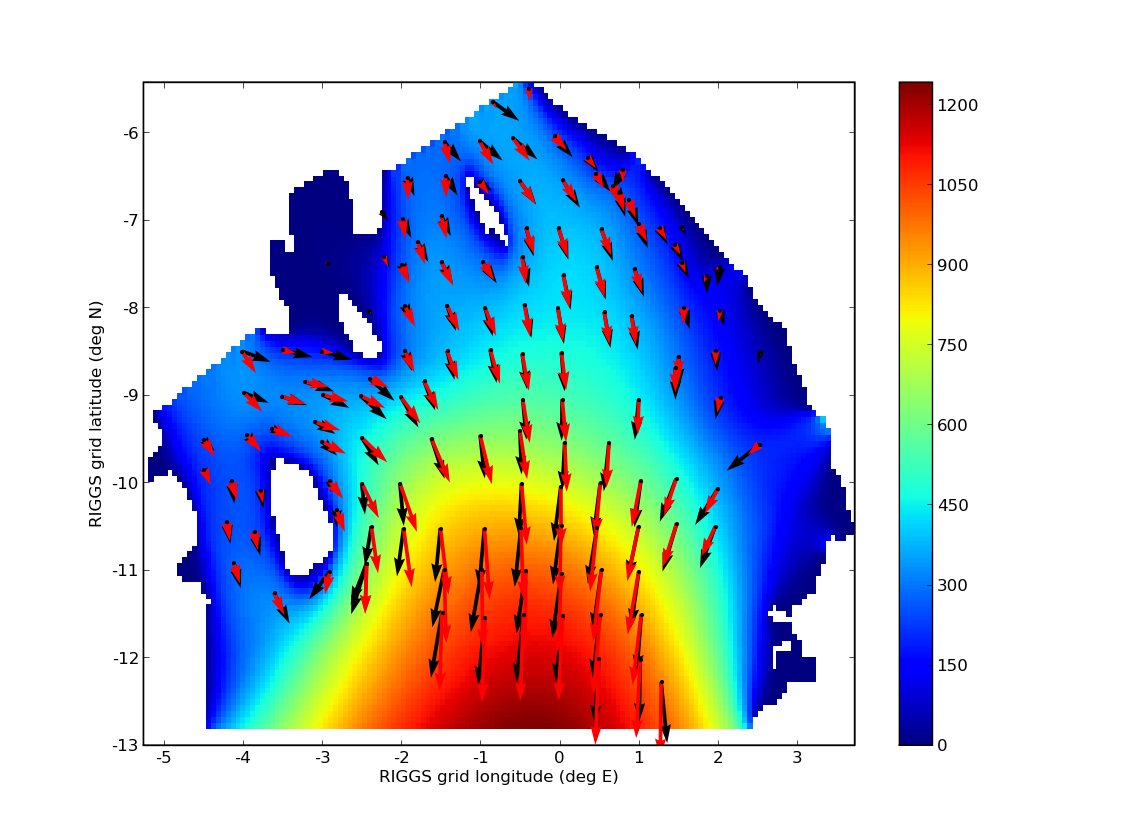
\includegraphics[width=3.5in,keepaspectratio=true]{figs/rossquiver}\quad 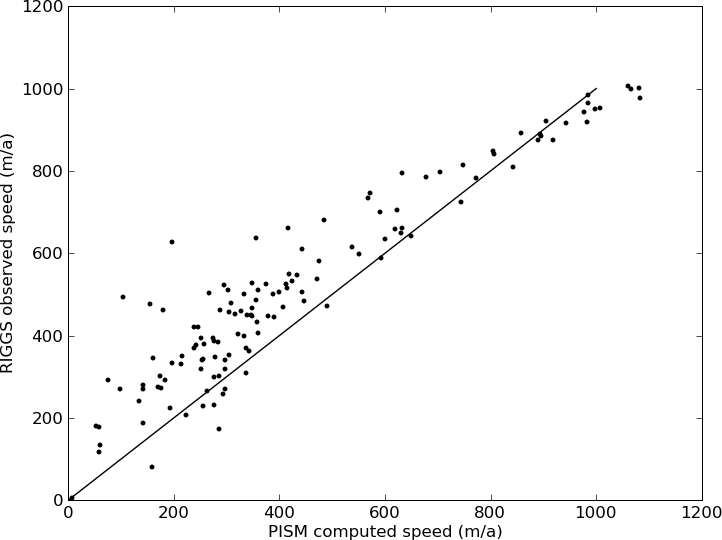
\includegraphics[width=2.5in,keepaspectratio=true]{figs/rossscatter}
\caption{\protect{\emph{Left}}: Color is speed in m/a.  Arrows are observed (black) and computed (red) velocities at RIGGS points.  \protect{\emph{Right}}: Comparison between modeled and observed speeds at RIGGS points; compare figure 2  in \cite{MacAyealetal}.}
\label{fig:rossmatlab}
\end{figure}


\clearpage\newpage
\section{Inside PISM: overviews of models, schemes, and sources}\label{sect:over}

\subsection{The continuum models in PISM}  Significant features of the continuum model approximated by the PISM include:\begin{itemize}
\item The inland ice sheet is modeled with the thermocoupled shallow ice approximation equations \cite{Fowler}, and some temperature-activated basal sliding is allowed.
\item Ice shelves and ice streams are modeled by shallow equations which describe flow by longitudinal strain rates and basal sliding.  These equations are different from the shallow ice approximation.  In shelves and streams the velocities are independent of depth within the ice.  The equations were originally established for ice shelves \cite{Morland,MorlandZainuddin,MacAyealetal,WeisGreveHutter}.  They were adapted for ice streams, as ``dragging ice shelves,'' by MacAyeal \cite{MacAyeal}; see also \cite{HulbeMacAyeal,SchoofStream}.
\item The regions of grounded ice in which the ice stream model is applied can be determined from mass balance velocities \cite{BamberVaughanJoughin}, from observed surface velocities, or from a plastic till assumption and the associated free boundary problem \cite{SchoofStream}.
\item A three dimensional age field is computed.
\item A temperature model for the bedrock under an ice sheet is included.
\item Geothermal flux which varies in the map-plane can be used.
\item Within the shallow ice sheet regions the model can use the constitutive relation of Goldsby and Kohlstedt \cite{GoldsbyKohlstedt,Peltieretal}.  For inclusion in this flow law, grain size can be computed using a age-grain size relation from the Vostok core data \cite{VostokCore}, for example.
\item The Lingle-Clark \cite{BLKfastearth,LingleClark} bed deformation model can be used.  It combines a spherical elastic earth and viscous half-space asthenosphere/mantle.  It generalizes the better known elastic lithosphere, relaxing asthenosphere (``ELRA'') model \cite{Greve2001}.  This model can be initialized by an observed bed uplift map \cite{BLKfastearth}, or even an uplift map computed by an external model like that in \cite{IvinsJames2005}.\end{itemize}

Many of the parts of the model described above are optional.  For instance, the Paterson-Budd-Glen \cite{PatersonBudd} flow can replace the Goldsby-Kohlstedt law, a simple isostasy model can be substituted for the more sophisticated one, and so on.  Options can be chosen at the command line as described in section \ref{sect:options} above.

The following features are \emph{not} included in the continuum model, and would (or will) require major additions:
\begin{itemize}
\item Inclusion of all components of the stress tensor (i.e.~longitudinal stresses within the shallow ice approximation region and additional shear stress components in shelves/streams) through either an intermediate order scheme (e.g.~\cite{Blatter,Hindmarsh06}) or the full Stokes equations \cite{Fowler}.
\item A model for water--content within the ice.  In the current model the ice is \emph{cold} and not \emph{polythermal}; compare \cite{Greve}.  On the other hand, in the current model the energy used to melt the ice within a given column, if any, is conserved.  In particular, a layer of basal melt water evolves by conservation of energy in the column.  This layer can activate basal sliding and its latent heat energy is available for refreezing.
\item A model for basal water mass conservation in the map-plane; compare \cite{JohnsonFastook}.
\item A fully spherical Earth deformation model, for example one descended from the Earth model of \cite{Peltier}.
\end{itemize}


\subsection{The numerical schemes in PISM}  Significant features of the numerical methods in PISM include:\begin{itemize}
\item Verification \cite{Roache} is a primary concern and is built into the code.  Nontrivial verifications are available for isothermal ice sheet flow \cite{BLKCB}, thermocoupled sheet flow \cite{BB,BBL}, conservation in ice and bedrock \cite{BuelerTestK}, the earth deformation model \cite{BLKfastearth}, the coupled (ice flow)/(earth deformation) system in an isothermal and pointwise isostasy  case \cite{BLKfastearth}, ice shelf flow (preprint), and ice stream flow based on failing plastic bed \cite{SchoofStream}.
\item The code is \emph{structurally} parallel.  In fact, the PETSc toolkit is used at all levels \cite{petsc-user-ref}.  PETSc manages the MPI-based communication between processors, and provides an interface to parallel numerical linear algebra and other numerical functions.
\item The grid can be chosen at the command line.  Regridding can be done at any time, for example taking the result of a rough grid computation and interpolating it onto a finer grid.
\item A moving boundary technique is used for the temperature equation which does not stretch the vertical in a singular manner; the Jenssen \cite{Jenssen} change of variables is not used.
\item The model uses an explicit time stepping method for flow and a partly implicit method for temperature.  Advection of temperature is upwinded \cite{MortonMayers}.  As described  in  \cite{BBL}, reasonably rigorous stability criteria are applied to the time-stepping scheme, including a diffusivity-based criteria for the explicit mass continuity scheme and a CFL criteria \cite{MortonMayers} for temperature/age advection.
\item The local truncation error is generically first order (i.e.~$O(\Delta x,\Delta y,\Delta z,\Delta t)$).
\item The shallow shelf approximation (SSA) \cite{WeisGreveHutter} is used to determine velocity in the ice shelf and ice stream regions.  Like the full non-Newtonian Stokes equations, they are nonlinear and nonlocal equations for the velocity given the geometry of the streams and shelves and given the ice temperature.  They are solved by straightforward iteration of linearized equations with numerically-determined (vertically-averaged) viscosity.  Either plastic till or linear drag is allowed.  As with all of PISM, the numerical approximation is finite difference.  The linearized finite difference equations are solved by any of the Krylov subspace methods in PETSc \cite{petsc-user-ref}.
\item The bed deformation model is implemented by a new Fourier collocation (spectral) method \cite{BLKfastearth}.
\item Implementation is in C++ and is object-oriented.  For example, verification occurs in a derived class.
\end{itemize}


\subsection{The PISM source code} This ice sheet model is implemented as a collection of C++ object classes, the most central of which is \t{IceModel}.  Actually there are three basic classes to know about, all of which are in \verb|pism/src/base/|:
\begin{itemize}
\item \t{IceGrid}, which describes the shape of the grid and parallel
layout. This abstraction could be used to streamline transferring model data between
different grids.
\item \t{MaterialType}.  Various materials are derived from the class \t{MaterialType} which merely defines a couple physical constants. \t{IceType} is a derived class, but still an abstract class. which defines the physical properties of ice as a material.  Concrete classes derived from \t{IceType} are \t{ThermoGlenIce} (which uses the
EISMINT constants) and \t{GKIce} as well as \t{HybridIce}, which implements the Goldsby-Kohlstedt flow law \cite{GoldsbyKohlstedt}.\footnote{Actually, it is difficult or impossible to implement a complete Goldsby-Kohlstedt \t{IceType} because the inverse constitutive relation is required for computation of SSA velocity fields. \t{HybridIce} is Goldsby-Kohlstedt ice in the interior of the ice sheet and Glen ice in ice streams and
shelves.}  Similarly, there is \t{BedrockType} and \t{OceanType} which merely define
associated physical constants.
\item \t{IceModel} which contains myriad data structures, flags, PETSc \verb|Vec|s (below), and most of the methods and numerical methods of PISM.\end{itemize}

The methods for \t{IceModel} are many, as noted.  In addition to numerics, they initialize the model (from input data files or from formulas describing various exact solutions), they read user options, they allocate arrays in a distributed manner under PETSc (below), they control diagnostic viewers, they run the adaptive time-stepping mechanism, they report the state of PISM to the user, and they write out the model state to files.

A derived class of \t{IceModel} called \t{IceCompModel} is used for verification.  It has additional structures which allows \t{IceModel} to have compensatory sources and compute initial conditions from, and especially to report errors relative to, known exact solutions \cite{BLKCB,BBL,BB}.  Another derived class used for verification is \t{IceExactStreamModel}, which implements the exact solution described in \cite{SchoofStream}.

Other derived classes of \t{IceModel} are \t{IceEISModel}, \t{IceGRNModel}, and \t{IceROSSModel}.  These correspond to simplified geometry experiments, the EISMINT-Greenland, and the EISMINT-Ross ice shelf models described in this manual.

There are five established drivers which in essense just call constructors and destructors for \t{IceModel} or a derived class thereof, and tell it to go.  These are in the source files \verb|pgrn.cc|, \verb|pismd.cc|, \verb|pismr.cc|, \verb|pisms.cc|, and \verb|pismv.cc|.  These correspond to the executables \verb|pgrn|, \verb|pismd|, \verb|pismr|, \verb|pisms|, and \verb|pismv|, respectively.  These drivers do no computation but differ in which derived class is constructed and in how certain options are handled.  The driver \verb|pismr.cc| and its executable \verb|pismr| only use the base class \verb|IceModel|; it requires a pre-existing saved PISM model state to start.

The different derived classes generally invoke the same numerical procedures to handle the various partial differential equations of the continuum model.  In the case of \t{IceCompModel}, this fact is at the heart of the verification mechanism.

\subsection{PETSc: An overview for PISM users}  The PETSc library \cite{petsc-user-ref,petsc-efficient} provides essential support for distributed arrays and linear solvers in a parallel computing environment.  ``PETSc'' stands for ``Portable, Extensible Toolkit for Scientific Computation.''  It is a suite of data structures and routines in C for the scalable parallel solution of partial differential equations and their scientific applications.  Large parts of PETSc relate especially to finite-difference-type regular, rectangular grids but PETSc has been used for unstructured grids as well.  Documentation for PETSc is available from the web site at \url{http://www-unix.mcs.anl.gov/petsc/petsc-as/}.  PETSc employs the MPI standard for all message-passing communication.  PETSc is deliberately at a higher level of abstraction than MPI; PETSc protects the programmer from explicit consideration of message passing.

Most variables in a PETSc program are of newly-defined distributed types including
\begin{verbatim}
DA   da;
Vec  v;
KSP  ksp;
\end{verbatim}
In fact most of the PETSc types merely declare pointers but they should be regarded as objects (abstract data types).  The objects must be created with calls to functions like \t{DACreate2d()}, \t{VecCreate()}, etc.  They should be destroyed when they are not needed with calls to corresponding \t{Destroy()} functions.

\subsubsection*{Distributed arrays and vectors} PETSc has an abstract date type called a Distributed Array (DA). Objects of type DA contain
information about the grid and stencil. They can have information about coordinates, but
the code does not use this feature at present. Vectors are created with
\texttt{DAVecCreate()} and similar. These vectors will be distributed across the
processors as indicated by the distributed array.

There are two parameters of note: stencil type and stencil width.  The stencil types are
\verb|DA_STENCIL_STAR| and \verb|DA_STENCIL_BOX|.  They are generalizations of the five
point and nine point stencils typical of two dimensional discretizations respectively.  In
particular, \verb|DA_STENCIL_STAR| indicates that ghosted points (information owned by a
different processor) will be needed only along the coordinate axes while
\verb|DA_STENCIL_BOX| indicates that ghosted points will be needed in the box shaped
region surrounding each point.  The stencil width indicates how many points in each
direction will be needed.  We never need a stencil width greater than 1 and only need BOX
style stencils when gradient terms must be evaluated on a staggered grid ($h$ in SIA
velocity and $\bar{u},\bar{v}$ in computation of effective viscosity in SSA
velocity).  Keeping all other two dimensional vectors on a STAR type stencil
would reduce the necessary communication slightly, but would complicate the code.  For this
reason, all two dimensional vectors are kept on a box type distributed array.

The three dimensional distributed arrays are aligned so that they have the same horizontal
extent as the associated two dimensional distributed array, but have complete vertical
extent. One point of confusion is the redefinition of the $x,y,z$ axes. Contrary to the
PETSc default, our $z$ axis changes most rapidly through memory while the $x$ axis changes
most slowly. That is, our C style arrays will be addressed as \texttt{u[i][j][k]} where
$\texttt{i,j,k}$ are the coordinate indices in the directions $x,y,z$ respectively.

DA-based vectors can be accessed by \texttt{DAVecGetArray()} and restored with
\texttt{DAVecRestoreArray()}. The resulting pointer should be addressed using normal
multidimensional array indexing where values range over the global array.

PETSc DA based vectors can be ``local'' or ``global''. Local vectors include space for the
ghosted points. That is, when \texttt{DAVecGetArray()} is called, the resulting array can
be indexed on all the ghosted points. However, all vector operations act only on the local
portion. \texttt{DALocalToLocalBegin()} and then \texttt{DALocalToLocalEnd()} should be
called to update the ghost points before they will be needed. Global vectors do not hold
ghosted values, but array operations will act on the entire vector. Hence local vectors
typically need to be mapped to global vectors before viewing or using in a linear system.
This is achieved with \texttt{DALocalToGlobal()}.

\subsubsection*{Solving linear systems}
PETSc is designed for solving large, sparse systems in a distributed environment.
Iterative methods are the name of the game and especially Krylov subspace methods such as
conjugate gradients and GMRES. For consistency, all methods use the Krylov subspace
interface. For this, the user declares an object of type \texttt{KSP}. Various options can
be set and the preconditioner context can be extracted. PETSc has an options database
which holds command line options. To allow these options to influence the \t{KSP}, one
should call \t{KSPSetFromOptions()} prior to solving the system. The default method is
GMRES(30) with ILU preconditioning.

To solve the system, a matrix must be attached to the \t{KSP}. The first time
\t{KSPSolve()} is called, the matrix will be factored by the preconditioner and reused
when the system is called for additional right hand sides. The default matrix format is
similar to the Matlab \t{sparse} format. Each processor owns a range of rows. Elements in
matrices and vectors can be set using \t{MatSetValues()} and \t{VecSetValues()}. These
routines use the global indexing and can set values on any processor. The values are
cached until one calls \t{MatAssemblyBegin()} followed by \t{MatAssemblyEnd()} to
communicate the values.

In the SSA velocity computation, the solution and right hand side vectors are not DA
based.

The vector (field) components are interlaced and distributed. This seemed to be the
most straightforward method to solve the system (as opposed to using more advanced
features intended for multiple degrees of freedom on DA based vectors). This also allows
the matrix to have an optimal parallel layout.

\subsubsection*{PETSc utility functions}
The \t{PetscViewer} interface allows PETSc objects to be displayed. This can be in binary
to disk, in plain text to the terminal, in graphical form to an X server, to a running
instance of Matlab, etc. Typically, one will want to view an entire vector, not just the
local portion, so DA based local vectors are mapped to global vectors before viewing.

When viewing multiprocessor jobs, the display may have to be set on the command line, for instance as
\t{-display :0} or similar; this must be given as the final option.  For example,

\verb|mpiexec -n 2 pismv -test C -Mx 101 -My 101 -Mz 31 -y 1000 -d HT -display :0|

\noindent views a two processor run of test C.

PETSc allows the programmer to access command line arguments at any time during program
execution. This is preferable to using \t{getopt.h} for this purpose.

Quite ellaborate error tracing and performance monitoring is possible with PETSc.  All
functions return \t{PetscErrorCode} which should be checked by the macro \t{CHKERRQ()}.
Normally, runtime errors print traceback information when the program exits.  If this
information is not present, you may need to use a debugger which is accessible with the
command line options \verb|-start_in_debugger| and \verb|-on_error_attach_debugger|.  Also
consider options such as \verb|-log_summary| to get diagnostics written to the terminal.


%         References
\clearpage\newpage
\bibliography{ice_bib}
\bibliographystyle{siam}

\appendix

\clearpage\newpage
\section{PISM command line options}\label{sect:options}

Much of the behavior of PISM can be set at the command line by options.  For example, the command 

\verb|$  pismv -test C -Mx 61 -gk -e 1.2 -o foo|

\noindent includes five options ``\verb|-test|'', ``\verb|-Mx|'', ``\verb|-gk|'', ``\verb|-e|'', and ``\verb|-o|'',  The first of these options includes a single character argument, the second an integer argument, the third has no argument, the fourth has a floating point argument, and the fifth has a string argument.

The format of the option documentation below is

\centerline{``\optdefrestrict{optionname}{A}{B} Description.''}

\noindent Here ``A'' is the default value and ``\t{B}'' is a list of the allowed executables.  The option applies to all executables (\verb|pismr|, \verb|pisms|, \verb|pismv|) unless the allowed executables are specifically stated by giving ``[\t{B} \textsl{only}]''.

As PISM is a PETSc program, all PETSc options are available \cite{petsc-user-ref}.  See the next section, which recalls some of these PETSc options.
\bigskip

\optdef{adapt\und ratio}{0.12}  Adaptive time stepping ratio for the explicit scheme for the mass balance equation.

\opt{bed\und def\und iso} Compute bed deformations by simple pointwise isostasy.  Assumes that the bed at the starting time is in equilibrium with the load so the bed elevation is equal to the starting bed elevation minus a multiple of the increase in ice thickness from the starting time, roughly: $b(t,x,y) = b(0,x,y) - f [H(t,x,y) - H(0,x,y)]$.  Here $f$ is the density of ice divided by the density of the mantle.  See Test H in Verification section.

\opt{bed\und def\und lc} Compute bed deformations, caused by the changing load of the ice, using a viscoelastic earth model.  Uses the model and computational technique described in \cite{BLKfastearth}, based on the continuum model in \cite{LingleClark}.

\optrestrict{bif}{pismr, pgrn}  The model can be ``bootstrapped'' from certain NetCDF files using less than the full initial values for the system of evolution partial differential equations.  See sections \ref{sect:boot} for generalities and \ref{sect:green} for an example.  Compare \verb|-if|.

\optrestrict{bif\und legacy}{pant}  The model can be ``bootstrapped'' from certain NetCDF files dealing with antarctica (\verb|init.nc|).

\opt{constant\und hardness}  If this option is used then the velocities in ice shelves and streams (see \verb|-mv| below) are computed with a constant, temperature-independent hardness parameter $\bar B$.  In particular, the viscous stress term in the $x$-component (for example) of the SSA equations for ice shelves and ice streams is
	$$\ddx{}\left(2\nu H\left(2\ddx{u} + \ddy{v}\right)\right)$$
where 
	$$\nu = \frac{\bar B}{2} \left[\left(\ddx{u}\right)^2 + \left(\ddy{v}\right)^2 +
  \frac{1}{4} \left(\ddy{u} + \ddx{v}\right)^2 + \ddx{u}\ddy{v}\right]^{(1-n)/(2n)}.$$
Generally $\bar B$ is computed by a vertical-integral of a function of the temperature field.  If \verb|-constant_hardness| is used then $\bar B$ is set to the given value.

In the case of \verb|pismd -ross|, which performs the EISMINT Ross ice shelf intercomparison, a constant value $\bar B = 1.9 \times 10^8 \, \text{Pa}\, \text{s}^{1/3}$ is the default \cite{MacAyealetal}.

\optdef{constant\und nu}{30.0}  If this option is used then the velocities in ice shelves and streams (see \verb|-mv| below) are computed with a constant viscosity $\nu$; see the option \verb|-constant_hardness| above.  Generally the viscosity is computed by a nonlinear iteration.  With option \verb|-constant_nu|, this iteration does not occur.  If \verb|-constant_nu| is set then \verb|-constant_hardness| is ignored.  The argument is given in units of MPa a, and the default value is $30$ MPa a, the value given in \cite{Ritzetal2001}.

\optrestrict{ccl3}{pgrn -forcing}    Run EISMINT-GREENLAND climate control experiment. See section \ref{sect:green}

\opt{d}  Specifies diagnostic (X Windows) viewers.  See Appendix C.

\optdefrestrict{datprefix}{PISM}{pisms -ismip H}  Specify base name for ISMIP-HEINO deliverable \verb|.dat| files.  See also \verb|-no_deliver|.

\opt{dbig}  Specifies larger (about twice linear dimensions) diagnostic viewers.  See Appendix C.

\optdef{e}{1.0}  Flow enhancement factor.

\optrestrict{eo}{pismv}  Only evaluate the exact solution (don't do numerical approximation at all).  See section \ref{sect:verif}.

\optdefrestrict{eisII}{A}{pisms}  Choose single character name of EISMINT II \cite{EISMINT00} simplified geometry experiment.  Allowed values are A, B, C, D, E, F, G, H.

\optrestrict{forcing}{pgrn}    Uses a NetCDF file to apply changes in surface temperature and sea level. See section \ref{sect:green} for an example.

\opt{f3d}  Save the model state with additional full velocity field.  That is, save all scalar components $u(x,y,z)$, $v(x,y,z)$, $w(x,y,z)$ of the velocity field for $(x,y,z)$ everywhere in the three-dimensional computational box.  Not needed when using \verb|pismd|, for which saving the full three-dimensional velocity field is the default.  Has the effect of (roughly) doubling the size of the output model state NetCDF file.

\optrestrict{gk}{pisms,pismr}  Sets the flow law to Goldsby-Kohlstedt.  Same as \verb|-law 4|.  See \verb|-law| for more complete option choice of flow law.

\opt{grad\und from\und eta}  The surface gradient is usually computed by simple centered-differences on the surface elevation.  With this option it is computed by first transforming the thickness $H$ by $\eta = H^{(2n+2)/n}$ and then differentiating the sum of the thickness and the bed:
	$$\grad h = \grad H + \grad b = \frac{n}{(2n+2)} \eta^{(-n-2)/(2n+2)} \nabla \eta + \nabla b.$$
Here $b$ is the bed elevation and $h$ is the surface elevation.  Note that only $n=3$ is used in this transformation regardless of the chosen flow law.  The transformation may have benefits in that the surface value of the vertical velocity may be better behaved near the margin, e.~.g.~as in EISMINT II experiments, but this is not yet clear.  See \cite{CDDSV} for the technical explanation of this transformation and compare \cite{SaitoMargin}.

\opt{hold\und tauc}    Keep the current values of the till yield stress $\tau_c$.  That is, do not update them by the default model using the stored basal melt water.  Only effective if \verb|-ssa| and \verb|-plastic| are also set.  See documentation of option \verb|-plastic| for a description of the till yield stress model.

\optrestrict{gwl3}{pgrn}    Run EISMINT-GREENLAND greenhouse warming. See section \ref{sect:green}.

\opt{id}  Sets the x grid index at which a sounding diagnostic viewer (section \ref{sect:viewers}) is displayed.  The integer argument should be in the range $0,\dots,\text{\t{Mx}}-1$.  The default is $(\text{\t{Mx}}-1)/2$ at the center of the grid.  For example, \verb|pismv -test G -d t -id 10|.

\opt{if}  The model can be initialized (restarted) from a NetCDF file \verb|foo.nc| written by the model, e.g.~\verb|foo.nc| from \verb|-o foo -of n|.  Compare \verb|-bif|.

\opt{jd}  Sets the y grid index at which a sounding diagnostic viewer (section \ref{sect:viewers}) is displayed.  The integer argument should be in the range $0,\dots,\text{\t{My}}-1$.  The default is $(\text{\t{My}}-1)/2$ at the center of the grid.  For example, \verb|pismv -test G -d t -jd 10|.

\optdef{kd}{0}  Sets the z grid index at which map-plane diagnositic views are shown.  Compare \verb|pismv -test G -Mz 101 -d T| and \verb|pismv -test G -Mz 101 -d T -kd 50|.  See section \ref{sect:viewers}.

\optdef{law}{0}  Allows choice of thermocoupled flow law.  The options are in table \ref{tab:flowlaw} below.  Note that a ``flow law'' here means the function $F(\sigma,T,P,d)$ in the relation
	$$\dot \eps_{ij} = F(\sigma,T,P,d)\, \sigma_{ij}'$$
where $\dot \eps_{ij}$ is the strain rate tensor, $\sigma_{ij}'$ is the stress deviator tensor, $T$ is the ice temperature, $\sigma^2 = \frac{1}{2} \|\sigma_{ij}'\|_F$ so $\sigma$ is the second invariant of the stress deviator tensor, $P$ is the pressure, and $d$ is the grain size.  That is, we are addressing isotropic flow laws only, and one can choose the scalar function.  Note that the inverse form of such a flow law in needed for ice shelves and ice streams:
	$$\sigma_{ij}' = 2 \nu(\dot\eps,T,P,d)\,\dot \eps_{ij} $$
Here $\nu(\dot \eps,T,P,d)$ is the effective viscosity.  The need for this inverse form of the flow law explains the ``hybrid'' law \verb|-law 4| (or \verb|-gk|).

\begin{table}[ht]
\caption{Choosing the flow law.}\label{tab:flowlaw}
\small
\begin{tabular}{@{}llll}\hline
\textbf{Flow Law} & \textbf{Option} & \textbf{Comments and Reference} \\ \hline
Paterson-Budd law   &  \t{-law 0} &   Fixed Glen exponent $n=3$.  There is a split ``Arrhenius'' \\
  & & term $A(T) = A \exp(-Q/RT^*)$ where \\
  & & $(A = 3.615 \times 10^{-13}\, \text{s}^{-1}\, \text{Pa}^{-3}, Q = 6.0 \times 10^4\, \text{J}\, \text{mol}^{-1})$ if \\
  & & $T^* < 263$ K and $(A = 1.733 \times 10^{3}\, \text{s}^{-1}\, \text{Pa}^{-3}$, \\
  & & $Q = 13.9 \times 10^4\, \text{J}\, \text{mol}^{-1})$ if $T^* > 263$ K and \\
  & & where $T^*$ is the homologous temperature \cite{PatersonBudd}.  \\
\emph{Cold} part of Paterson-Budd    &  \t{-law 1} &   Regardless of temperature, the values for $T^*<263$ K in \\
  & & the Paterson-Budd law above apply.  This is the flow law \\
  & & used in the thermomechanically coupled exact solutions \\
  & & Tests \textbf{F} and \textbf{G} described in \cite{BBL,BB} \\
  & & and run by \verb|pismv -test F|,  \verb|pismv -test F|.  \\
\emph{Warm} part of Paterson-Budd     &  \t{-law 2} & Regardless of temperature, the values for $T^*>263$ K in \\
  & &  Paterson-Budd apply.    \\
Hooke law   &  \t{-law 3} &  Fixed Glen exponent $n=3$.  Here \\
  & & $A(T) = A \exp(-Q/(RT^*) + 3C (T_r - T^*)^\kappa)$; values of \\
  & & constants as in \cite{Hooke,PayneBaldwin}.   \\
Hybrid of Goldsby-Kohlstedt &  \t{-law 4} &     Goldsby-Kohlstedt law with a combination of exponents  \\
  \qquad and Paterson-Budd & & from $n=1.8$ to $n=4$ \cite{GoldsbyKohlstedt} in grounded \\
  & & shallow ice approximation regions.  Paterson-Budd flow \\
  & & for ice streams and ice sheets. See mask for SIA \\
  & & versus stream versus shelf by \verb|-d m|. \\
\hline
\normalsize	
\end{tabular}
\end{table}

\optdef{low\und temp}{200.0}  Set the temperature which PISM will regard as ``too low''.  Units in Kelvin.  Note that one kind of numerical error associated to the advection part of the conservation of energy scheme is for the maximum principle to be violated.  In that case temperatures appear at the next step which are outside the range of current temperatures.  PISM attempts to count such violations, and if the number is too great then the run is stopped.  See option \verb|-max_low_temps|.

\opt{Lx}  The x direction half-width of the computational box, in kilometers.  See section \ref{sect:usage}.

\opt{Ly}  The y direction half-width of the computational box, in kilometers.  See section \ref{sect:usage}.

\opt{Lz}  The height of the computational box for the ice (excluding the bedrock thermal model part).  See section \ref{sect:usage}.

\optdef{mato}{pism\und views}  Specifies the name of the \Matlab-readable file in which to save the views.  Use with \verb|-matv|, to set which views to save; if \verb|-matv| is not set then \verb|-mato| has no effect.

\opt{matv}  Specifies which \Matlab ``views'' to save at end of run.  See Appendix C for list of single character names of the views.  The default is for \emph{no} \Matlab views.  See \verb|-mato| for setting the name of the \Matlab-readable file in which to save the views.  Typically the user will write \verb|-mato foo -matv HT0c| to save four views in the \Matlab-readable ASCII file \verb|foo.m|.

\optdef{maxdt}{60.0}  The maximum time-step in years.  The adaptive time-stepping scheme will make the time-step shorter than this as needed for stability, but not longer.  See section \ref{sect:usage}.

\optdef{max\und low\und temps}{10}  Specify the number (a nonnegative integer) of allowed low temp violations per time step.  Note these are reported in detail (i.e.~with location) if \verb|-verbose| is set.  Note that one kind of numerical error associated to the advection part of the conservation of energy scheme is for the maximum principle to be violated.  In that case temperatures appear at the next step which are outside the range of current temperatures.  PISM attempts to count such violations, and if the number is too great then the run is stopped.  See option \verb|-low_temp| for the cutoff low temperature.

\optdef{Mbz}{1}  Number of grid points in the bedrock for the bedrock thermal model.  The highest grid point corresponds to the base of the ice $z=0$, and so \t{Mbz}$>1$ is required to actually have bedrock thermal model.  Note this option is unrelated to the bed deformation model (glacial isostasy model); see option \verb|-bed_def| for that.

\optrestrict{Mmax}{pisms -eisII}  Set value of $M_{\text{max}}$ for EISMINT II.

\optdef{mu\und sliding}{3.17e-11}  The sliding law parameter in SIA regions of the ice.

\optdef{Mx}{61}  Number of grid points in x horizontal direction.

\optdef{My}{61}  Number of grid points in y horizontal direction.

\optdef{Mz}{31}  Number of grid points in z (vertical) direction.

\opt{no\und mass}  Forces PISM not to change the ice thickness.  No time steps of the mass conservation equation are computed.

\optrestrict{no\und report}{pismv}  Do not report errors at the end of a verification run.

\optdef{no\und spokes}{0}  The strain heating term can be smoothed by non-physical averaging the neighboring horizontal neighbors (those which are within the ice) \cite{BBL}.  The integer parameter controls the number of neighboring grid points over which the average is computed.  For instance, \verb|-no_spokes 0| is no smoothing while \verb|-no_spokes 3| is smoothing over the 3-neighborhood of horizontal grid points, that is, over a distance of \verb|3*dx|.

\opt{no\und temp}  Do not change temperature or age values within the ice.  That is, do not do time steps of energy conservation and age equation.

\optdef{o}{unnamed.nc} Give name of output file: \verb|-o foo| writes an output file named \verb|foo.nc|.  See the description of option \verb|-if|.  Default name is \verb|unnamed.nc| under \verb|pismr|, \verb|simp_exper.nc| under \verb|pisms|, and \verb|verify.nc| under \verb|pismv|.

\opt{ocean\und kill}  If used with input from a NetCDF initialization file which has ice-free ocean mask, will zero out ice thicknesses in areas that were ice-free ocean at time zero.  Has no effect when used in conjunction with \verb|-no_mass|.

\optdef{of}{n}  Format of output file(s).  Possible values are \verb|n| for model state written to a NetCDF file \verb|foo.nc| and \verb|m| for selected variables written to an ASCII Matlab file \verb|foo.m|.  PISM can be restarted using \verb|-if| from the output \verb|.nc| files.  Multiple files can be written, for instance, \verb|-o foo -of nm| writes both \verb|foo.nc| and \verb|foo.m|.

\optrestrict{pause}{pismd -ross,pismv -test I,pismv -test J}    Pause for given number of seconds at the end of the run when the results are displayed.

\opt{pdd}  Turns on the positive degree day model (which is off by default for \verb|pismr|, \verb|pisms|, and \verb|pismv|).  See subsection \ref{subsect:pdd}.

\optdef{pdd\und factor\und ice}{0.008}  The amount of ice, measured in meters, which is melted per positive degree day.  In units of $\text{m}\!\phantom{|}^\circ\text{C}^{-1}\text{day}^{-1}$.  See subsection \ref{subsect:pdd}.

\optdef{pdd\und factor\und snow}{0.003}  The amount of snow, measured in meters ice-equivalent, which is melted per positive degree day.  In units of $\text{m}\phantom{|}^\circ\text{C}^{-1}\text{day}^{-1}$.  See subsection \ref{subsect:pdd}.

\optdef{pdd\und refreeze}{0.6}  Fraction of melted snow, from positive degree day melting, which locally refreezes as ice (and therefore adds to accumulation).  See subsection \ref{subsect:pdd}.

\opt{pdd\und repeatable}  Base the randomness specified by \verb|pdd_std_dev| on a predictable seed.  Makes no difference if \verb|pdd_std_dev| is 0.0.  Allows runs with positive \verb|pdd_std_dev| to be identically repeated.  See subsection \ref{subsect:pdd}.

\optdef{pdd\und std\und dev}{0.0}  Standard deviation of temperature increment added each day to temperature cycle in positive degree day model.  Units of $\phantom{|}^\circ\text{C}$.  See subsection \ref{subsect:pdd}.

\optdef{pdd\und summer\und warming}{15.0}  Difference between peak summer temperature and mean annual temperature at each grid location.  Units of $\phantom{|}^\circ\text{C}$.  See subsection \ref{subsect:pdd}.

\opt{plastic}  Use Schoof's plastic till model for ice streams at all grounded points on the ice sheet.  Must be used along with \verb|-ssa| to turn on the solution of the SSA (shallow shelf approximation).  See subsection \ref{subsect:plastic}.  See options \verb|-plastic_reg|, \verb|-plastic_c0|, \verb|-plastic_phi|, and \verb|-plastic_pwfrac|, all of which control the plastic till model in various ways.

Indeed, we describe the role of the parameters for the plastic till model as follows: The effective pressure $N$ on the till is
	$$N = P - p = (1 - (\mathtt{pwfrac}) \lambda) P$$
where $P = \rho g H$ is the overburden or hydrostatic pressure at the base (see Paterson \cite{Paterson}, pp.~168--169) and $p = (\mathtt{pwfrac}) \lambda P$ is the pore water pressure in the till.  Here $\lambda$ is a pure number, $0\le \lambda \le 1$, measuring the amount of available basal water.  In particular, $\lambda = 0$ if the base is frozen, while $\lambda$ is a linear function of the stored basal melt water (see \verb|-d L|), up to the fixed maximum amount of stored basal melt water.  Thus our model says that when there is a lot (the maximum) amount of available basal water, $p= (\mathtt{pwfrac}) P$; the default value for $\mathtt{pwfrac}$ is 0.95.

Note that Paterson gives this formula for the till yield stress
	$$\tau_c = c_0 + \mu N, \qquad \mu = \tan \phi,$$
while Schoof \cite{SchoofStream} formula (2.4) gives this one
	$$\tau_c = \mu N,$$
with zero till cohesion.  We allow a positive till cohesion, though the default is zero, and we describe $\mu$ as the tangent of the friction angle $\phi$.

\optdef{plastic\und c0}{0.0}  Set the value of the till cohesion in the plastic till model.  The value is a pressure, given in kPa.  Only effective if used with \verb|-plastic| and \verb|-ssa|.

Note Schoof \cite{SchoofStream} formula (2.4) uses $c_0 = 0$.

\optdef{plastic\und pwfrac}{0.95}  Set what fraction of overburden pressure is assumed as the till pore water pressure.  Only relevant at basal points where there is a positive amount of basal water.  The value is a pure number.  Only effective if used with \verb|-plastic| and \verb|-ssa|.

\optdef{plastic\und reg}{0.01 m/a}    Set the value of $\eps$ regularization of plastic till; this is the second ``$\eps$'' in formula (4.1) in \cite{SchoofStream}.  Only effective if used with \verb|-plastic| and \verb|-ssa|.

\optdef{plastic\und phi}{30.0}  Set the till friction angle.  The value is an angle $\phi$, given in degrees, and the coefficient $\mu$ in formula (2.4) in \cite{SchoofStream} is computed from $\theta$ by this formula:
	$$\mu = \tan\left(\frac{\pi}{180} \theta\right).$$
Only effective if used with \verb|-plastic| and \verb|-ssa|.

\opt{regrid}  See section \ref{sect:usage}.

\opt{regrid\und vars}  See section \ref{sect:usage}.

\optdef{reg\und length\und schoof}{1000 km}  Set the ``$L$'' in formula (4.1) in \cite{SchoofStream}.  To use the regularization described by Schoof, one must set \verb|-ssa_eps 0.0| to turn off the other regularization mechanism, otherwise there is a double regularization.

\optdef{reg\und vel\und schoof}{1 m/a}  Set the \emph{first} ``$\eps$'' in formula (4.1) in \cite{SchoofStream}.  To use the regularization described by Schoof, one must set \verb|-ssa_eps 0.0| to turn off the other regularization mechanism, otherwise there is a double regularization.  Use \verb|-plastic_reg| above to set the second ``$\eps$'' in formula (4.1) of \cite{SchoofStream}.

\optrestrict{Rel}{pisms -eisII}    Set value of $R_{\text{el}}$ for EISMINT II.

\optrestrict{ross}{pisms}    Run the EISMINT Ross ice shelf validation \cite{MacAyealetal}.  Requires data from \url{http://homepages.vub.ac.be/~phuybrec/eismint/iceshelf.html}.

\optrestrict{Sb}{pisms -eisII}    Set value of $S_b$ for EISMINT II.

\opt{ssa}  Use the equations of the shallow shelf approximation \cite{MacAyeal,Morland,SchoofStream,WeisGreveHutter} for ice shelves and dragging ice shelves (i.e.~ice streams) where so-indicated by the mask.  To view the mask use \verb|-d m|.  See also \verb|-plastic| and \verb|-super|.

\optdef{ssa\und eps}{1.0e15}  The numerical scheme for the shallow shelf approximation  \cite{WeisGreveHutter} computes an effective viscosity which which depends on velocity and temperature.  After that computation, this constant is added to the effective viscosity (to keep it bounded away from zero).  The units are kg $\text{m}^{-1}\,\text{s}^{-1}$. 

In fact there is a double regularization by default because the Schoof regularization mechanism described in equation (4.1) of \cite{SchoofStream} is also used.  Turn off this lower bound mechanise by \verb|-ssa_eps 0.0| to exclusively use the Schoof regularization mechanism; see \verb|-reg_vel_schoof| and \verb|-reg_length_Schoof| below.  Note \verb|-ssa_eps| is set to zero automatically when running \verb|pismv -test I|.

\optdef{ssa\und maxi}{300}  This option sets the maximum allowed number of nonlinear iterations in solving the shallow shelf approximation.  One should usually use option \verb|-ssa_rtol| to control convergence of the nonlinear iteration.

\optdef{ssa\und rtol}{1.0e-4}  The numerical scheme for the shallow shelf approximation \cite{WeisGreveHutter} does a nonlinear iteration wherein velocities (and temperatures) are used to compute a vertically-averaged effective viscosity which is used to solve the equations for horizontal velocity.  Then the new velocities are used to recompute an effective viscosity, and so on.  This option sets the relative change tolerance for the effective viscosity.

In particular, the nonlinear part of the iteration requires that successive values $\nu^{(k)}$ of the vertically-averaged effective viscosity satisfy
	$$\frac{\|(\nu^{(k)} - \nu^{(k-1)}) H\|_2}{\|\nu^{(k)} H\|_2} \le \text{ssa\und rtol}$$
in order to end the iteration with $\nu = \nu^{(k)}$.  See also \verb|-ksp_rtol|, a PETSc option below, as one may want to require a high relative tolerance for the linear iteration as well.

\optrestrict{ssl2}{pgrn}    Run EISMINT-GREENLAND steady state experiment level 2. See section \ref{sect:green}.

\optrestrict{ssl3}{pgrn}    Run EISMINT-GREENLAND steady state experiment level 3.  Use with option \verb|-gk|: ``\verb|pgrn -ssl3 -gk|.  See section \ref{sect:green}.

\optrestrict{ST}{pisms -eisII}    Set value of $S_T$ for EISMINT II.

\opt{super}  Superpose the velocity fields from the SIA and SSA models.  That is, add the velocity fields which result from the SIA and SSA versions of the balance of momentum equations.  Also has the effect of the option \verb|-mu_sliding 0.0|, that is, the SIA-type sliding law is set to zero so that all basal sliding is controlled by the SSA model.  Only effective if used with \verb|-ssa|.

\optdef{tempskip}{1}  Number of mass-balance steps to perform before a temperature step is executed.  A maximum value of \verb|-tempskip 5| is recommended to avoid too many CFL violations.

\optdefrestrict{test}{A}{pismv}  Choose which verification test to run by giving its single character name.  See section \ref{sect:verif}.

\optdefrestrict{till\und phi}{20.0,5.0}{pisms -eisII I -ssa -plastic}  Set the till friction angle map special to the modification of EISMINT II experiment I discussed in subsection \ref{subsect:plastic}.

\optrestrict{Tmin}{pisms -eisII}    Set value of $T_{\text{min}}$ for EISMINT II.

\optrestrict{track\und Hmelt}{pisms -eisII}    Turn on the part of the conservation of energy model which accumulates (tracks) locally-stored basal melt water.

\opt{verbose}   Increased verbosity of standard output.  Can be given without argument (``\verb|-verbose|'') or with a level which is one of the integers 0,1,2,3,4,5 (``\verb|-verbose 2|'').  The full scheme is given in table \ref{tab:verbosity}.

\begin{table}[h]
\caption{Controlling the verbosity level to standard out.}\label{tab:verbosity}
\begin{tabular}{@{}llll}\hline
\textbf{Level} & \textbf{Option} & \textbf{Meaning} \\ \hline
   0  &  \t{-verbose 0} &   never print to standard out \emph{at all}; no warnings appear  \\
   1  &  \t{-verbose 1} &   only warning messages and other high priority messages will appear  \\
   2  &  [\t{-verbose 2}] & default verbosity    \\
   3  &  \t{-verbose 3} &   somewhat verbose; expanded description of grid at start  \\
      &  or \quad \t{-verbose} &  and expanded information in summary    \\
   4  &  \t{-verbose 4} &     \\
      &  or \quad \t{-vverbose} &  more verbose    \\
   5  &  \t{-verbose 5} &     \\
      &  or \quad \t{-vvverbose} &  maximally verbose \\
\hline
\normalsize
\end{tabular}
\end{table}

\opt{vverbose}   See table \ref{tab:verbosity}.

\opt{vvverbose}   See table \ref{tab:verbosity}.

\optdef{y}{1000} Number of model years to run.

\opt{ye} Model year at which to end the run.

\optdef{ys}{0} Model year at which to start the run.

\begin{comment}
% don't document ismip -H options
 \optrestrict{force\und quarter\und year}{pisms -ismip H}  ISMIP-HEINO specifies rigid $0.25$ year time steps.  This will violate both the diffusivity and the CFL parts of the adaptive time-stepping scheme.  This option overrides the adaptime time-stepping and does $0.25$ year time steps anyway; \emph{will probably cause blowup so don't bother}.

\optdefrestrict{ismip}{H}{pisms}  Choose ISMIP simplified geometry experiment.  Only ``H'' for HEINO is allowed at this time.

\optdefrestrict{run}{ST}{pisms -ismip H}  ISMIP-HEINO has several run names: ST, T1, T2, B1, B2, S1, S2, S3.

\optrestrict{time1}{pisms -ismip H}  ISMIP-HEINO requires writing 2D planform \verb|.dat| files at four times in the interval $[150,200]\times 10^{3}$ years.  This specifies the time.  Note \verb|test/showheino.m| will compute the time from the other \verb|.dat| files.

\optrestrict{time2}{pisms -ismip H}  See \verb|-time1| explanation.

\optrestrict{time3}{pisms -ismip H}  See \verb|-time1| explanation.

\optrestrict{time4}{pisms -ismip H}  See \verb|-time1| explanation.
\end{comment}


\clearpage\newpage
\section{PETSC command line options (for PISM users)}  All PETSc programs accept command line options which control the manner in which PETSc distributes jobs among parallel processors, how it solves linear systems, what additional information it provides, and so on.  The PETSc manual (\url{http://www.mcs.anl.gov/petsc/petsc-as/snapshots/petsc-current/docs/manual.pdf}) is the complete reference on these options.  Here we list some that are perhaps most useful to PISM users.

\opt{da\und processors\und x}  Number of processors in x direction.

\opt{da\und processors\und y}  Number of processors in y direction.

\opt{display}  The option \verb|-display :0| seems to frequently be needed to let PETSc use Xwindows when running multiple processes.  \emph{It must be given as a \emph{final} option, after all the others.}

\opt{help}  Gives PISM help message and then a brief description of many PETSc options.

\opt{info}  Gives excessive information about PETSc operations during run.  Option \verb|-verbose| for PISM (above) is generally more useful, except possibly for debugging.

\optdef{ksp\und rtol}{1e-5}  For solving the SSA equations with high resolution on multiple processors, it is recommended that this be tightened (set lower than the default).  For example, 

\verb|$  mpiexec -n 8 pismv -test I -Mx 5 -My 769|

\noindent works poorly on a certain machine, but

\verb|$  mpiexec -n 8 pismv -test I -Mx 5 -My 769 -ksp_rtol 1e-10|

\noindent works fine.

\optdef{ksp\und type}{gmres}  Based on one processor evidence from \verb|pismv -test I|, the following are possible choices in the sense that they work and allow convergence at some reasonable rate: \t{cg}, \t{bicg}, \t{gmres}, \t{bcgs}, \t{cgs}, \t{tfqmr}, \t{tcqmr}, and \t{cr}.  It appears \t{bicg}, \t{gmres}, \t{bcgs}, and \t{tfqmr}, at least, are all among the best.

\opt{log\und summary}  At the end of the run gives a performance summary and also a synopsis of the PETSc configuration in use.

\optdef{pc\und type}{ilu}   Several options are possible, but for solving the ice stream and shelf equations we recommend only \t{bjacobi}, \t{ilu}, and \t{asm}.  Of these it is not currently clear which is fastest; they are all about the same for \verb|pismv -test I| with high tolerances (e.g.~\verb|-ssa_rtol 1e-7| \verb|-ksp_rtol 1e-12|).

\opt{v}   Show version number of PETSc.


\clearpage \newpage
\section{PISM viewers: Graphical and \Matlab}\label{sect:viewers}

\subsubsection*{Viewing the PISM state}  Basic graphical views of the changing state of a PISM ice model are available at the command line by using the options ``\t{-d}'' and ``\t{-dbig}'' with additional arguments.  For instance:

\verb|$  pismv -test G -d hTf -dbig 0|

\noindent shows a map-plane views of surface elevation (``\t{h}''), temperature at the level specified by \t{-kd} (``\t{T}''), rate of change of thickness (``\t{f}'') and of horizontal ice speed at the surface (``\t{0}'', i.e.~zero).

The option \t{-d} is followed by a space and then a list of single-character names of the diagnositic viewers.  The option \t{-dbig} works exactly the same way, with the same list of single-character names available.  The bigger viewers take precedence, so that ``\t{-d hT -dbig T}'' shows only two viewers, namely a regular size viewer for surface elevation and a larger viewer for temperature.
\medskip

The same views of the PISM model can be saved \emph{at the end of the run} to a \Matlab-readable ASCII file by the same single character names.  (At this point, \emph{most} of the names are allowed; see the list below.)  We will call these ``\Matlab views''.  For instance,

\verb|$  pismv -test G -mato foo -matv hTf0|

\noindent will save surface elevation (``\t{h}''), temperature at the level specified by \t{-kd} (``\t{T}''), rate of change of thickness (``\t{f}'') and of horizontal ice speed at the surface (``\t{0}'') in an ASCII file \verb|foo.m|.  To use \verb|foo.m| at the \Matlab command line, make sure the \Matlab path includes the directory with \verb|foo.m|.  Then just do

\verb|>> foo|

\noindent You will be able to plot the surface elevation (for example) by

\verb|>> imagesc(x,y,flipud(H')), axis square, colorbar|

\noindent but you can also use the \Matlab tools \verb|contour|, \verb|surf|, and so on.  (\emph{The necessity to do} ``\verb|flipud(H')|'' \emph{to get the expected orientation, that is, the necessity of doing both do a transpose \emph{and} a} \verb|flipud|, \emph{is for various deep reasons too complicated to explain here.  Feel free to enquire, but \emph{sorry} in the meantime.})


\subsubsection*{Single character names (for each view)}  The single character diagnostic viewer and \Matlab views names are:
\newcommand{\notMat}{(\emph{NOT available as a} \Matlab \emph{view}.)\xspace\xspace}

\verb|0|:\quad Map-plane view of horizontal ice speed (magnitude of velocity) at the surface of the ice in meters per year.

\verb|1|:\quad Map-plane view of $x$-component of horizontal ice velocity at the \emph{surface} of the ice in meters per year.

\verb|2|:\quad Map-plane view of $y$-component of horizontal ice velocity at the \emph{surface} of the ice in meters per year.

\verb|3|:\quad Map-plane view of vertical ice velocity at the \emph{surface} of the ice in meters per year; positive values are upward velocities.

\verb|4|:\quad Map-plane view of $x$-component of horizontal ice velocity at the \emph{base} of the ice in meters per year.

\verb|5|:\quad Map-plane view of $y$-component of horizontal ice velocity at the \emph{base} of the ice in meters per year.

\verb|B|:\quad Map-plane view of basal drag coefficient $\beta$ for ice stream regions.  $\beta$ has units of Pa s $\text{m}^{-1}$.  Displayed as log base ten of $\beta$.

\verb|C|:\quad Map-plane view of basal till yield stress $\tau_c$, under plastic till ice stream model.  Units of kPa.

\verb|D|:\quad \notMat Map-plane view of diffusivity coefficient $D$ in mass balance equation in $\text{m}^2/s$.  Meaningful only in regions of shallow ice flow.

\verb|E|:\quad Map-plane view of age of the ice, in years.

\verb|F|:\quad Map-plane view of basal geothermal heat flux, in milliWatts per meter squared.

\verb|G|:\quad Map-plane view of grain size, in millimeters.  Displayed at chosen elevation above base; see option \verb|-kd|.

\verb|H|:\quad Map-plane view of thickness in meters.

\verb|L|:\quad Map-plane view of basal melt water \emph{thickness} in meters.

\verb|P|:\quad \notMat (\emph{ONLY available for }\t{pismv}.)  Map-plane view of comPensatory heating term $\Sigma_C$ in thermocoupled verification tests F and G.  Displayed at chosen elevation above base; see option \verb|-kd|.

\verb|Q|:\quad Map-plane view of basal driving stress $f_{\text{basal}} = \rho g H |\grad h|$.  Units of kPa.  Note that this quantity is the effective shear stress at the base in the SIA.  It is also the (magnitude of the) driving source term in the SSA, for both ice streams and ice shelves.  Compare to \verb|-d C|, the view of the till yield stress, when using the plastic till ice stream model.

\verb|R|:\quad Map-plane view of basal frictional heating in milliWatts per meter squared.

\verb|S|:\quad Map-plane view of strain heating term $\Sigma$ in temperature equation, in Kelvin per year.  Displayed at chosen elevation above base; see option \verb|-kd|.

\verb|T|:\quad Map-plane view of absolute ice temperature in Kelvin.  Displayed at chosen elevation above base; see option \verb|-kd|.

\verb|U|:\quad Map-plane view of vertically averaged horizontal velocity in the $x$-direction \emph{on the staggered grid} which is offset by positive one in $i$ direction;  in meters per year.  (\emph{Meaningful only in technical/numerical context}; use \verb|u| generally.)

\verb|V|:\quad Map-plane view of vertically averaged horizontal velocity in the $y$-direction \emph{on the staggered grid} which is offset by positive one in $j$ direction;  in meters per year.  (\emph{Meaningful only in technical/numerical context}; use \verb|v| generally.)

\verb|X|:\quad Map plane view of $x$-component of horizontal velocity, in meters per year.  Displayed at chosen elevation above base; see option \verb|-kd|.

\verb|Y|:\quad Map plane view of $y$-component of horizontal velocity, in meters per year.  Displayed at chosen elevation above base; see option \verb|-kd|.

\verb|Z|:\quad Map plane view of vertical velocity, in meters per year.  Displayed at chosen elevation above base; see option \verb|-kd|.

\verb|a|:\quad Map-plane view of accumulation in meters per year.

\verb|b|:\quad Map-plane view of bed elevation in meters above sea level.

\verb|c|:\quad Map-plane view of horizontal speed, namely the absolute value of the vertically-averaged horizontal velocity.  Displayed as log base ten of speed in meters per year.

\verb|e|:\quad Age in a vertical column (sounding); in years.  See \verb|-id|, \verb|-jd| to set sounding location.

\verb|f|:\quad Map-plane view of thickening rate of the ice, in meters per year.

\verb|g|:\quad Grain size in a vertical column (sounding); in millimeters.  See \verb|-id|, \verb|-jd| to set sounding location.

\verb|h|:\quad Map-plane view of ice surface elevation in meters above sea level.

\verb|i|:\quad Map-plane view of vertically-averaged effective viscosity times thickness; on $i$ offset grid.  Only meaningful in ice streams and shelves.

\verb|j|:\quad Map-plane view of vertically-averaged effective viscosity times thickness; on $i$ offset grid.  Only meaningful in ice streams and shelves.

\verb|k|:\quad \notMat Iteration monitor for the Krylov subspace routines (KSP) in Petsc.  Shows norm of residual versus iteration number.  Has same effect as PETSc option \verb|-ksp_monitor_draw|.

\verb|l|:\quad Map-plane view of basal melt \emph{rate} in meters per year.

\verb|m|:\quad Map-plane view of mask for flow type:  \textbf{1} = grounded shallow ice sheet flow,  \textbf{2} = dragging ice shelf, \textbf{3} = floating ice shelf, \text{7} = ice free ocean (in original input file).

%\verb|N|:\quad Produces two viewers, namely the $i$ offset and $j$ offset grid versions of the rate of change of the vertically-averaged effective viscosity times thickness.  Only meaningful in ice streams and shelves.

\verb|n|:\quad Map-plane view of the log base ten of the vertically-averaged effective viscosity times thickness on the regular grid.  Only meaningful in ice streams and shelves.

\verb|p|:\quad Map-plane view of bed uplift rate in meters per year.

\verb|q|:\quad Map-plane view of basal sliding speed.  Displayed as log base ten of speed in meters per year.

\verb|r|:\quad Map-plane view of surface temperature in Kelvin.

\verb|s|:\quad Strain heating term $\Sigma$ in vertical column (sounding).  See \verb|-id|, \verb|-jd| to set sounding location.

\verb|t|:\quad Absolute ice temperature in vertical column (sounding).  Note this sounding extends into the bedrock, unlike the other soundings (e.g.~\verb|-d egsxyz|).  See \verb|-id|, \verb|-jd| to set sounding location.

\verb|u|:\quad Map-plane view of vertically averaged horizontal velocity in the $x$-direction;  in meters per year.

\verb|v|:\quad Map-plane view of vertically averaged horizontal velocity in the $y$-direction;  in meters per year.

\verb|x|:\quad $x$-component of horizontal velocity in vertical column (sounding).  See \verb|-id|, \verb|-jd| to set sounding location.

\verb|y|:\quad $y$-component of horizontal velocity in vertical column (sounding).  See \verb|-id|, \verb|-jd| to set sounding location.

\verb|z|:\quad Vertical velocity ($w$-component of velocity) in vertical column (sounding).  See \verb|-id|, \verb|-jd| to set sounding location.



\clearpage \newpage
\section{Python scripts for PISM modeling}\label{sect:scripts}

The following scripts, among others, are found in subdirectory \verb|pism/test/|.

\subsubsection*{\Large{\texttt{fill\und missing.py}}}  [FILL IN DOCUMENTATION]

\verb|fill_missing.py -i data.nc -v b,H,Ts -o data_smoothed.nc|.  Note that \emph{each} of the listed variables must have an attribute named \verb|missing_value|.


\subsubsection*{\Large{\texttt{series.py}}}  This Python script postprocesses the standard output of \verb|pismr|, \verb|pisms|, \verb|pgrn|, or \verb|pismv| if it is stored in a text file.  (That is, standard output from the PISM \emph{evolution} executables.  Output from \verb|pismd|, an executable for diagnostic runs, is not supported.)

Time series are extracted from the text file containing the standard output.  Typically this means time series for ice sheet volume, area, melt fraction, thickness at the center of the grid, and temperature of the base of the ice at the center of the grid.  Also the time series for the time step length itself is extracted.  These time series are put into a one-dimensional NetCDF file.

An example usage is

\verb|$  pisms -eisII A -Mx 61 -My 61 -Mz 201 -y 5000 >> eisIIA.out|

\verb|$  series.py -f eisIIA.out -o eisIIA_series.nc|

\verb|$  ncview eisIIA_series.nc|

For temperature-dependent SIA \verb|pismv| output (tests F,G,K) run as above, but for isothermal SIA \verb|pismv| output (tests A,B,C,D,E,L) add the option ``\verb|-i|'':

\verb|$  pismv -test C >> testC.out|

\verb|$  series.py -i -f testC.out -o testC_series.nc|

\noindent In this case \verb|series.py| only extracts time series for volume, area, and central thickness.

Note that the small number of digits reported in the standard output from the PISM executables may limit the utility of the resulting time series.  That is, the time series may mostly show discrete steps which result from the small number of digits reported rather than from the (unreported) full precision volume, area, etc.

\verb|series.py| takes the following options.  They have both a short form and a long form, \emph{a la} GNU; the default is in brackets:

\optoptdef{f}{file}{foo.txt} Specify the name of the text file.

\optoptdef{i}{isopismv}{False} If ``\verb|-i|'' is given then \verb|series.py| assumes the text file came from using \verb|pismv| on an isothermal SIA verification test.

\optoptdef{o}{out}{series\und out.nc} Give the full name, including the \verb|.nc| extension, of the output NetCDF file.



\subsubsection*{\Large{\texttt{ssl\und exper.py}}}  This Python script is actually special to the EISMINT-Greenland experiment described in section \ref{sect:green}.  It is worth documenting here in part because it is an example of using scripts with \href{http://nco.sourceforge.net/}{NCO}, and in part because we need to document its options to help readers of section \ref{sect:green}.

[FIXME: DOCUMENT THE OPTIONS!]


\subsubsection*{\Large{\texttt{verifynow.py}}}  This Python script organizes the process of verifying PISM.  It specifies standard refinement paths for each of the tests described in section \ref{sect:verif}.  It runs the tests, times them, and summarizes the numerical errors reported at the end.

Three example usages are \begin{itemize}
\item ``\verb|verifynow.py|'' without options will use one processor and do three levels of refinement; this command is equivalent to \verb|verifynow.py -n 1 -l 3 -t CGIJ|
\item ``\verb|verifynow.py -n 8 -l 5 -t J --prefix=bin/ --mpido=mpirun/|'' will use \verb|mpirun -np 8| \verb|bin/pismv| as the command and do five levels (the maximum) of refinement only on test J
\item ``\verb|verifynow.py -n 40 -l 5 -t ABCDEFGIJKL|'' will use forty processors to do all possible verification as managed by \verb|verifynow.py|; don't run this unless you have a big computer and you are prepared to wait
\end{itemize}

\verb|verifynow.py| takes the following options.  They have both a short form and a long form, \emph{a la} GNU; the default is in brackets:

\optoptdef{l}{levels}{3} specifies number of levels of refinement; $1,2,3,4,5$ are allowed values

\optoptdef{m}{mpido}{\texttt{mpiexec}} how to run PISM as an MPI program

\optoptdef{n}{nproc}{1} specify number of processors to use

\optoptdef{p}{prefix}{} where the PISM executable \verb|pismv| is located

\optoptdef{t}{tests}{CGIJ} which tests to run

\medskip
Note that timing information is also given in the \verb|verifynow.py| output.  Therefore performance, including parallel performance, can be assessed along with accuracy.

The exact meaning of the various errors reported by \verb|pismv|, which appear in a \verb|verifynow.py| output as well, is currently only documented in the source files \verb|pism/src/verif/iceCompModel.cc|, \verb|pism/src/verif/iCMthermo.cc|, and \verb|pism/src/verif/iceExactSSAModel.cc|.  


\subsubsection*{\Large{\texttt{vnreport.py}}}  This Python script postprocesses the standard output of \verb|verifynow.py| above.  The output is converted into graphs using \verb|gnuplot|.  Example graphs are Figures \ref{fig:thickerrsB} through \ref{fig:temperrsK} in section \ref{sect:verif}.

The basic use is this:

\verb|$  verifynow.py -n 2 -l 3 -t BGIK >> foo.txt|

\verb|$  vnreport.py -f foo.txt -t B -e 'geometry' -o thickerrs|

\noindent (Figures \ref{fig:thickerrsB} through \ref{fig:temperrsK} in section \ref{sect:verif} were actually generated by a level five (``\verb|-l 5|'') \verb|verifynow.py| run, but that takes a lot of computer time.)

The \verb|verifynow.py| run will take a while.  The \verb|vnreport.py| run will (quickly) look at \verb|foo.txt| and extract the geometry (thickness) numerical errors and refinement path and build a \verb|.eps| (encapsulated Postscript) image like that in Figure \ref{fig:thickerrsB}.

The \verb|Makefile| in the documentation directory \verb|pism/doc/| gives more example usages.  In fact, \verb|vnreport.py| is primarily used to automate the creation of this manual.  This \verb|Makefile| also shows how to use Ghostscript to convert the \verb|.eps| images to \verb|.png| (Portable Network Graphics) format.

\verb|vnreport.py| takes the following options:

\optoptdef{e}{error}{'geometry'} which kind of error to look for; for example, with test E the valid possibilities are \verb|'geometry'| and \verb|'base vels'|

\optoptdef{f}{file}{foo.txt} name of the text file containing the \verb|verifynow.py| report

\optoptdef{o}{out}{report} prefix of output file name; if ``\verb|-t G -o bar|'' then output file is named ``\verb|bar_G.eps|''

\optoptdef{t}{test}{A} the test for which to find the \verb|verifynow.py| report; only one value allowed

\optoptdef{x}{exclude}{} specify tags of errors to exclude from the figure


%\printindex
\end{document}
